\chapter{Database Design}
\section{Processing, Storing, and Organising Data}
\subsection{OLTP and OLAP}
\subsubsection{How should we organize and manage data?}
\begin{itemize}
    \item \textbf{Schemas}: How should my data be logically organized?
    \item \textbf{Normalization}: Should my data have minimal dependency and redundency?
    \item \textbf{Views}: What joins will be done most often?
    \item \textbf{Access control}: Should all users of the data have same level of access
    \item \textbf{DBMS}: How do i pick between SQL and NoSQL options?
\end{itemize}
It depends on the intended use of the data.

\subsubsection{Approaches to processing data}
OLTP : Online Transaction Processing \\
OLTP Tasks
\begin{itemize}
    \item Find the price of a book
    \item Update latest customer Transaction
    \item Keep track of employee hours
\end{itemize}

OLAP : Online Analytical Processing \\
OLAP Tasks
\begin{itemize}
    \item Calculate books with best profit margin
    \item Find most loyal customers
    \item Decide employee of the month
\end{itemize}

\begin{table}[H]
    \centering
    \caption{OLAP vs OLTP}
    \label{tab:ProcessingDataApproaches}
    \begin{tabular}{lll}
        & OLTP & OLAP \\
        Purpose & support daily transaction & report and analyze data \\
        Design & application-oriented & subject-oriented \\
        Data & up-to-date, operational & consolidated, historical \\
        Size & snapshot, gigabytes & archive, terabytes \\
        Queries & simple transactions \& frequent & complex, aggregate queries \& limited updates \\
        Users & thousands & hundreds
    \end{tabular}
\end{table}

\begin{figure}[H]
    \centering
    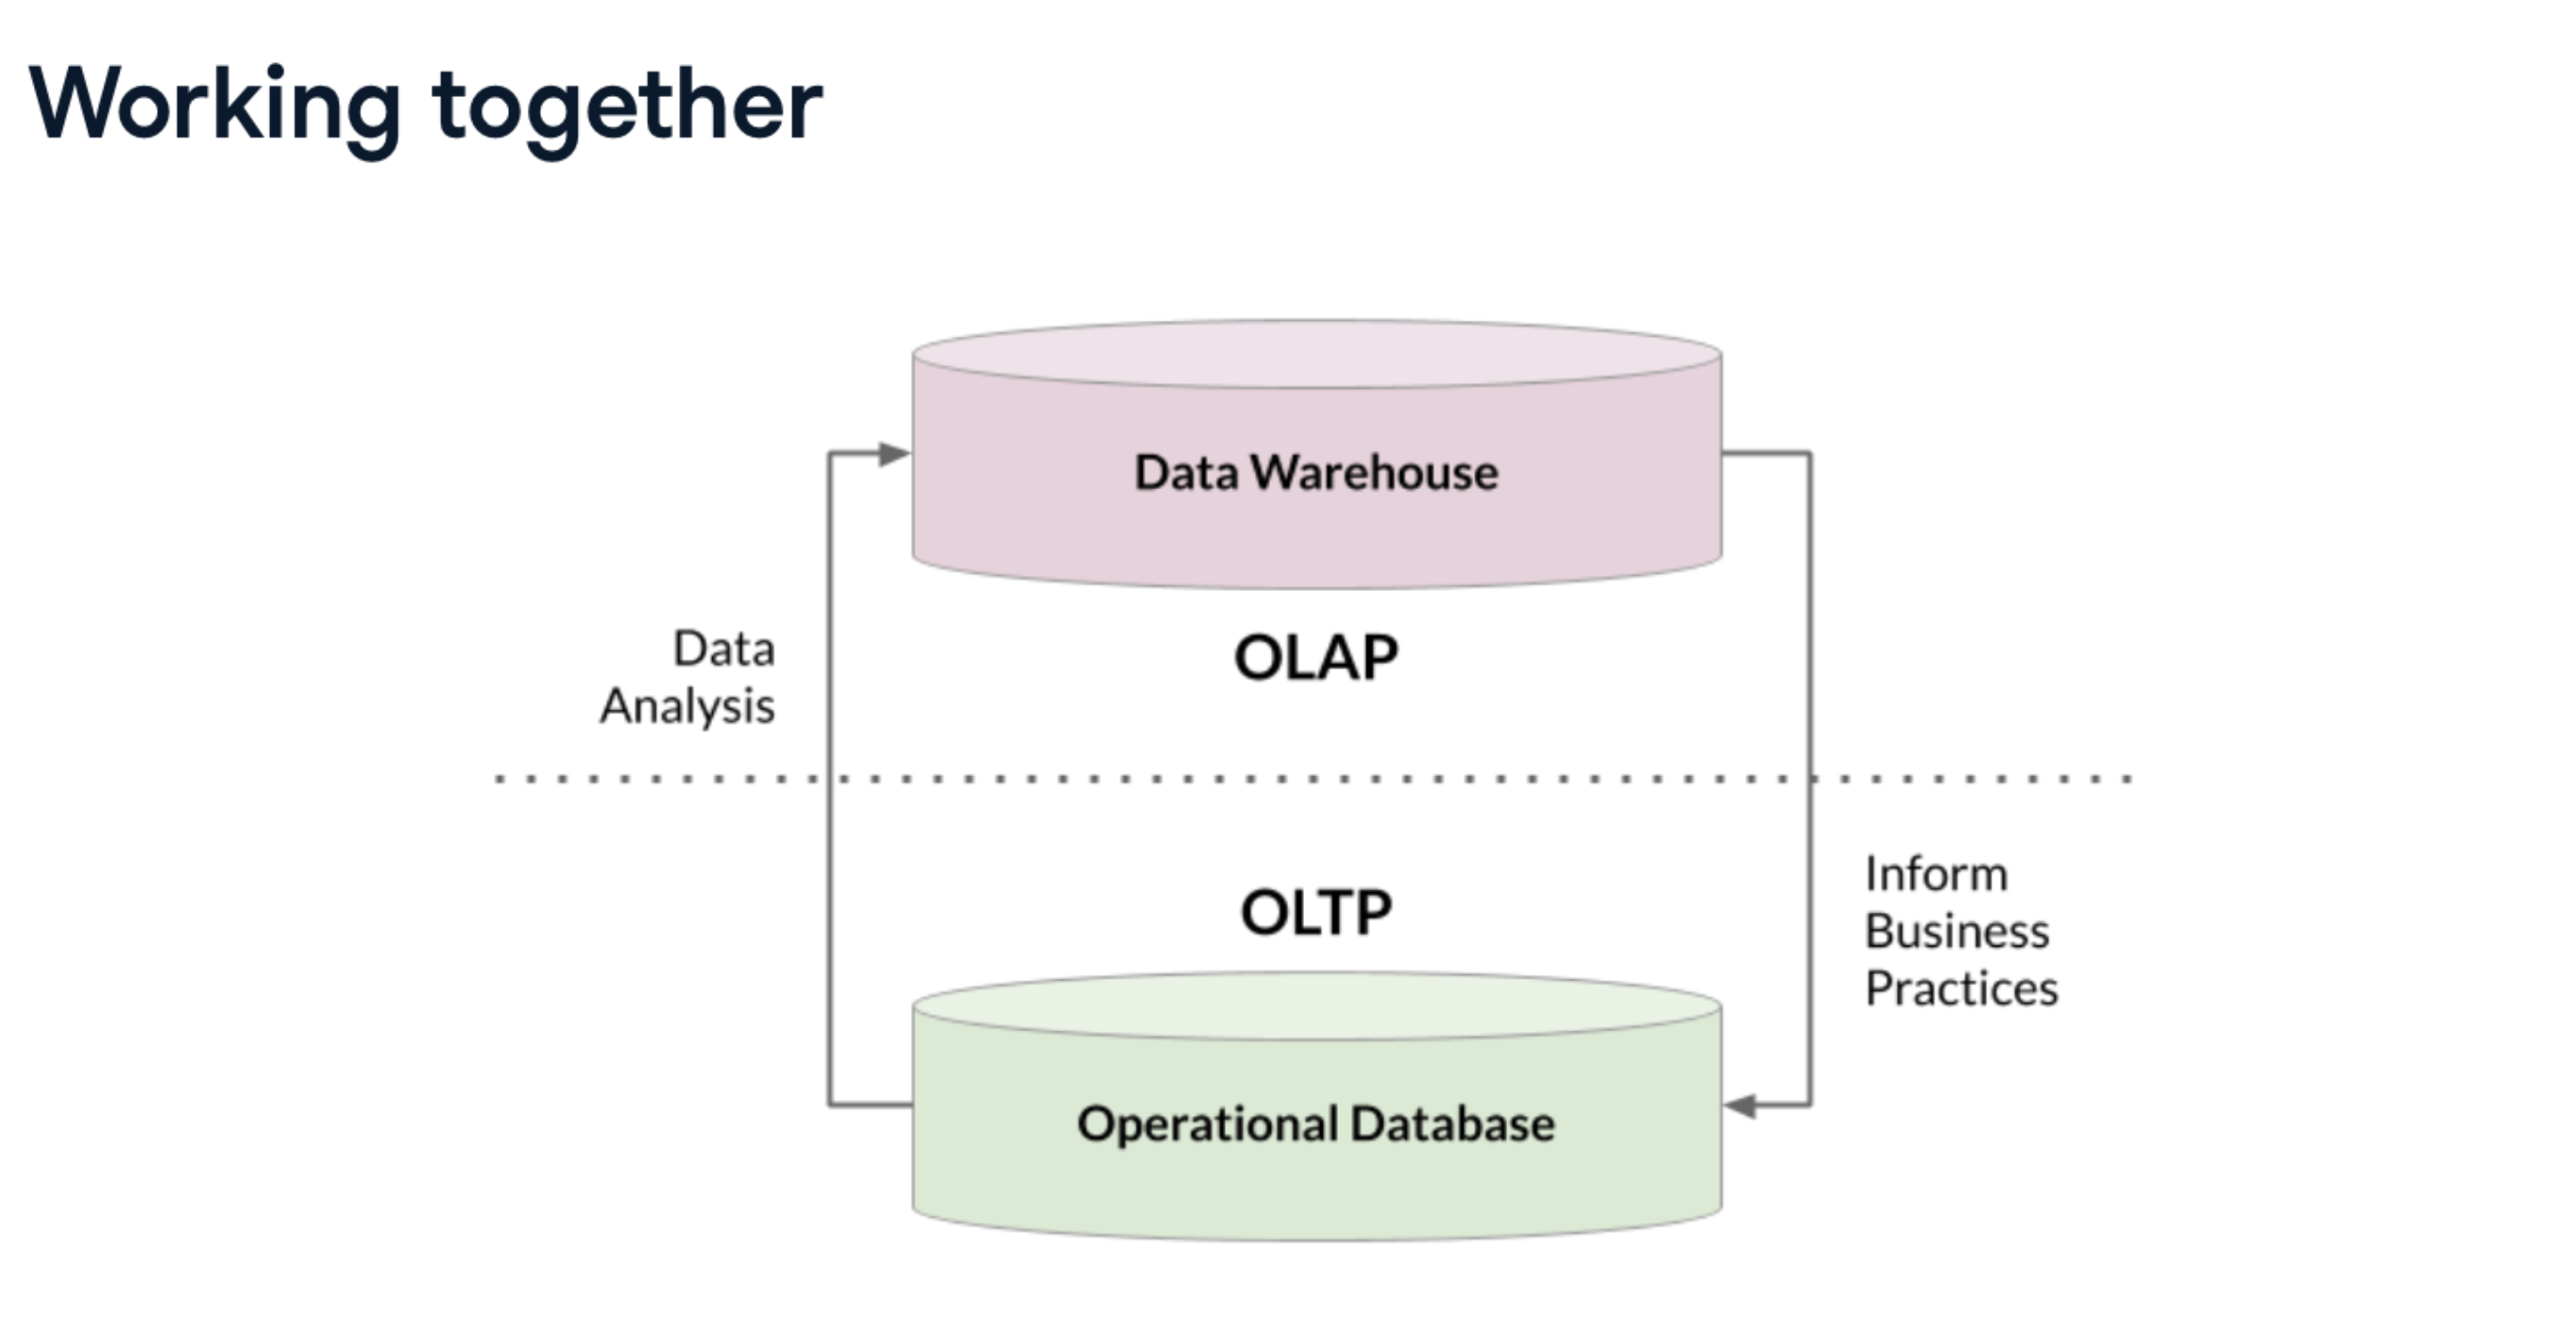
\includegraphics[width=1.0\textwidth]{figures/WorkingTogether.png}
    \caption{Working together}
    \label{fig:WorkingTogether}
\end{figure}

\subsection{Storing data}
\subsubsection{Structuring data}
\begin{enumerate}
    \item Structured data 
    \begin{itemize}
        \item Follow a Schema
        \item Easier to analyze
        \item Defined data types \& relationships \\
        e.g., SQL, tables in a relational database
    \end{itemize}
    \item Unstructured data
    \begin{itemize}
        \item Schemaless
        \item Makes up most of data in the world \\
        e.g., photos, chat logs, MP3
    \end{itemize}
    \item Semi-structured data
    \begin{itemize}
        \item Does not follow larger Schema
        \item Self-describing structure \\
        e.g., NoSQL, XML, JSON
    \end{itemize}
\end{enumerate}

\subsubsection{Storing data beyond traditional Databases}
\begin{itemize}
    \item Traditional database \\
    For storing real-time relational structured data -> OLTP
    \item Data warehouses \\
    For analyzing archived structured data -> OLAP
    \item Data Lakes \\
    For storing data of all structures = flexibility and scalability \\
    For analyzing big data
\end{itemize}

\subsubsection{Data warehouses}
\begin{itemize}
    \item Optimized for analytics - \textbf{OLAP}
    \begin{itemize}
        \item Organized for reading/aggregating data
        \item Usually readonly
    \end{itemize}
    \item Contains data from multiple sources
    \item Massively Parallel Processing (MPP)
    \item Typically uses a denormalizing scheme and dimensional modeling \\
    Example : Redshift, Azure SQL Data Warehouse, Google BigQuery
\end{itemize}

\subsubsection{Data Marts}
\begin{itemize}
    \item Subset of data warehouses
    \item Dedicated to specific topic
\end{itemize}

\subsubsection{Data Lakes}
\begin{itemize}
    \item Stores all types of data at a lower costs \\
    e.g. raw, operational databases, IoT device logs, real-time, relational and non relational
    \item Retains all data and can take up petabytes
    \item Schema-on-read as opposed to Schema-on-write 
    \item Need to catalog data otherwise becomes a \textbf{data swamp}
    \item Run \textbf{big data analytics} using services such as \textbf{Apache Spark} and \textbf{Hadoop}
    \begin{itemize}
        \item Useful for deep learning and data discovery because activity require so much data 
    \end{itemize}
\end{itemize}

\begin{figure}[H]
    \centering
    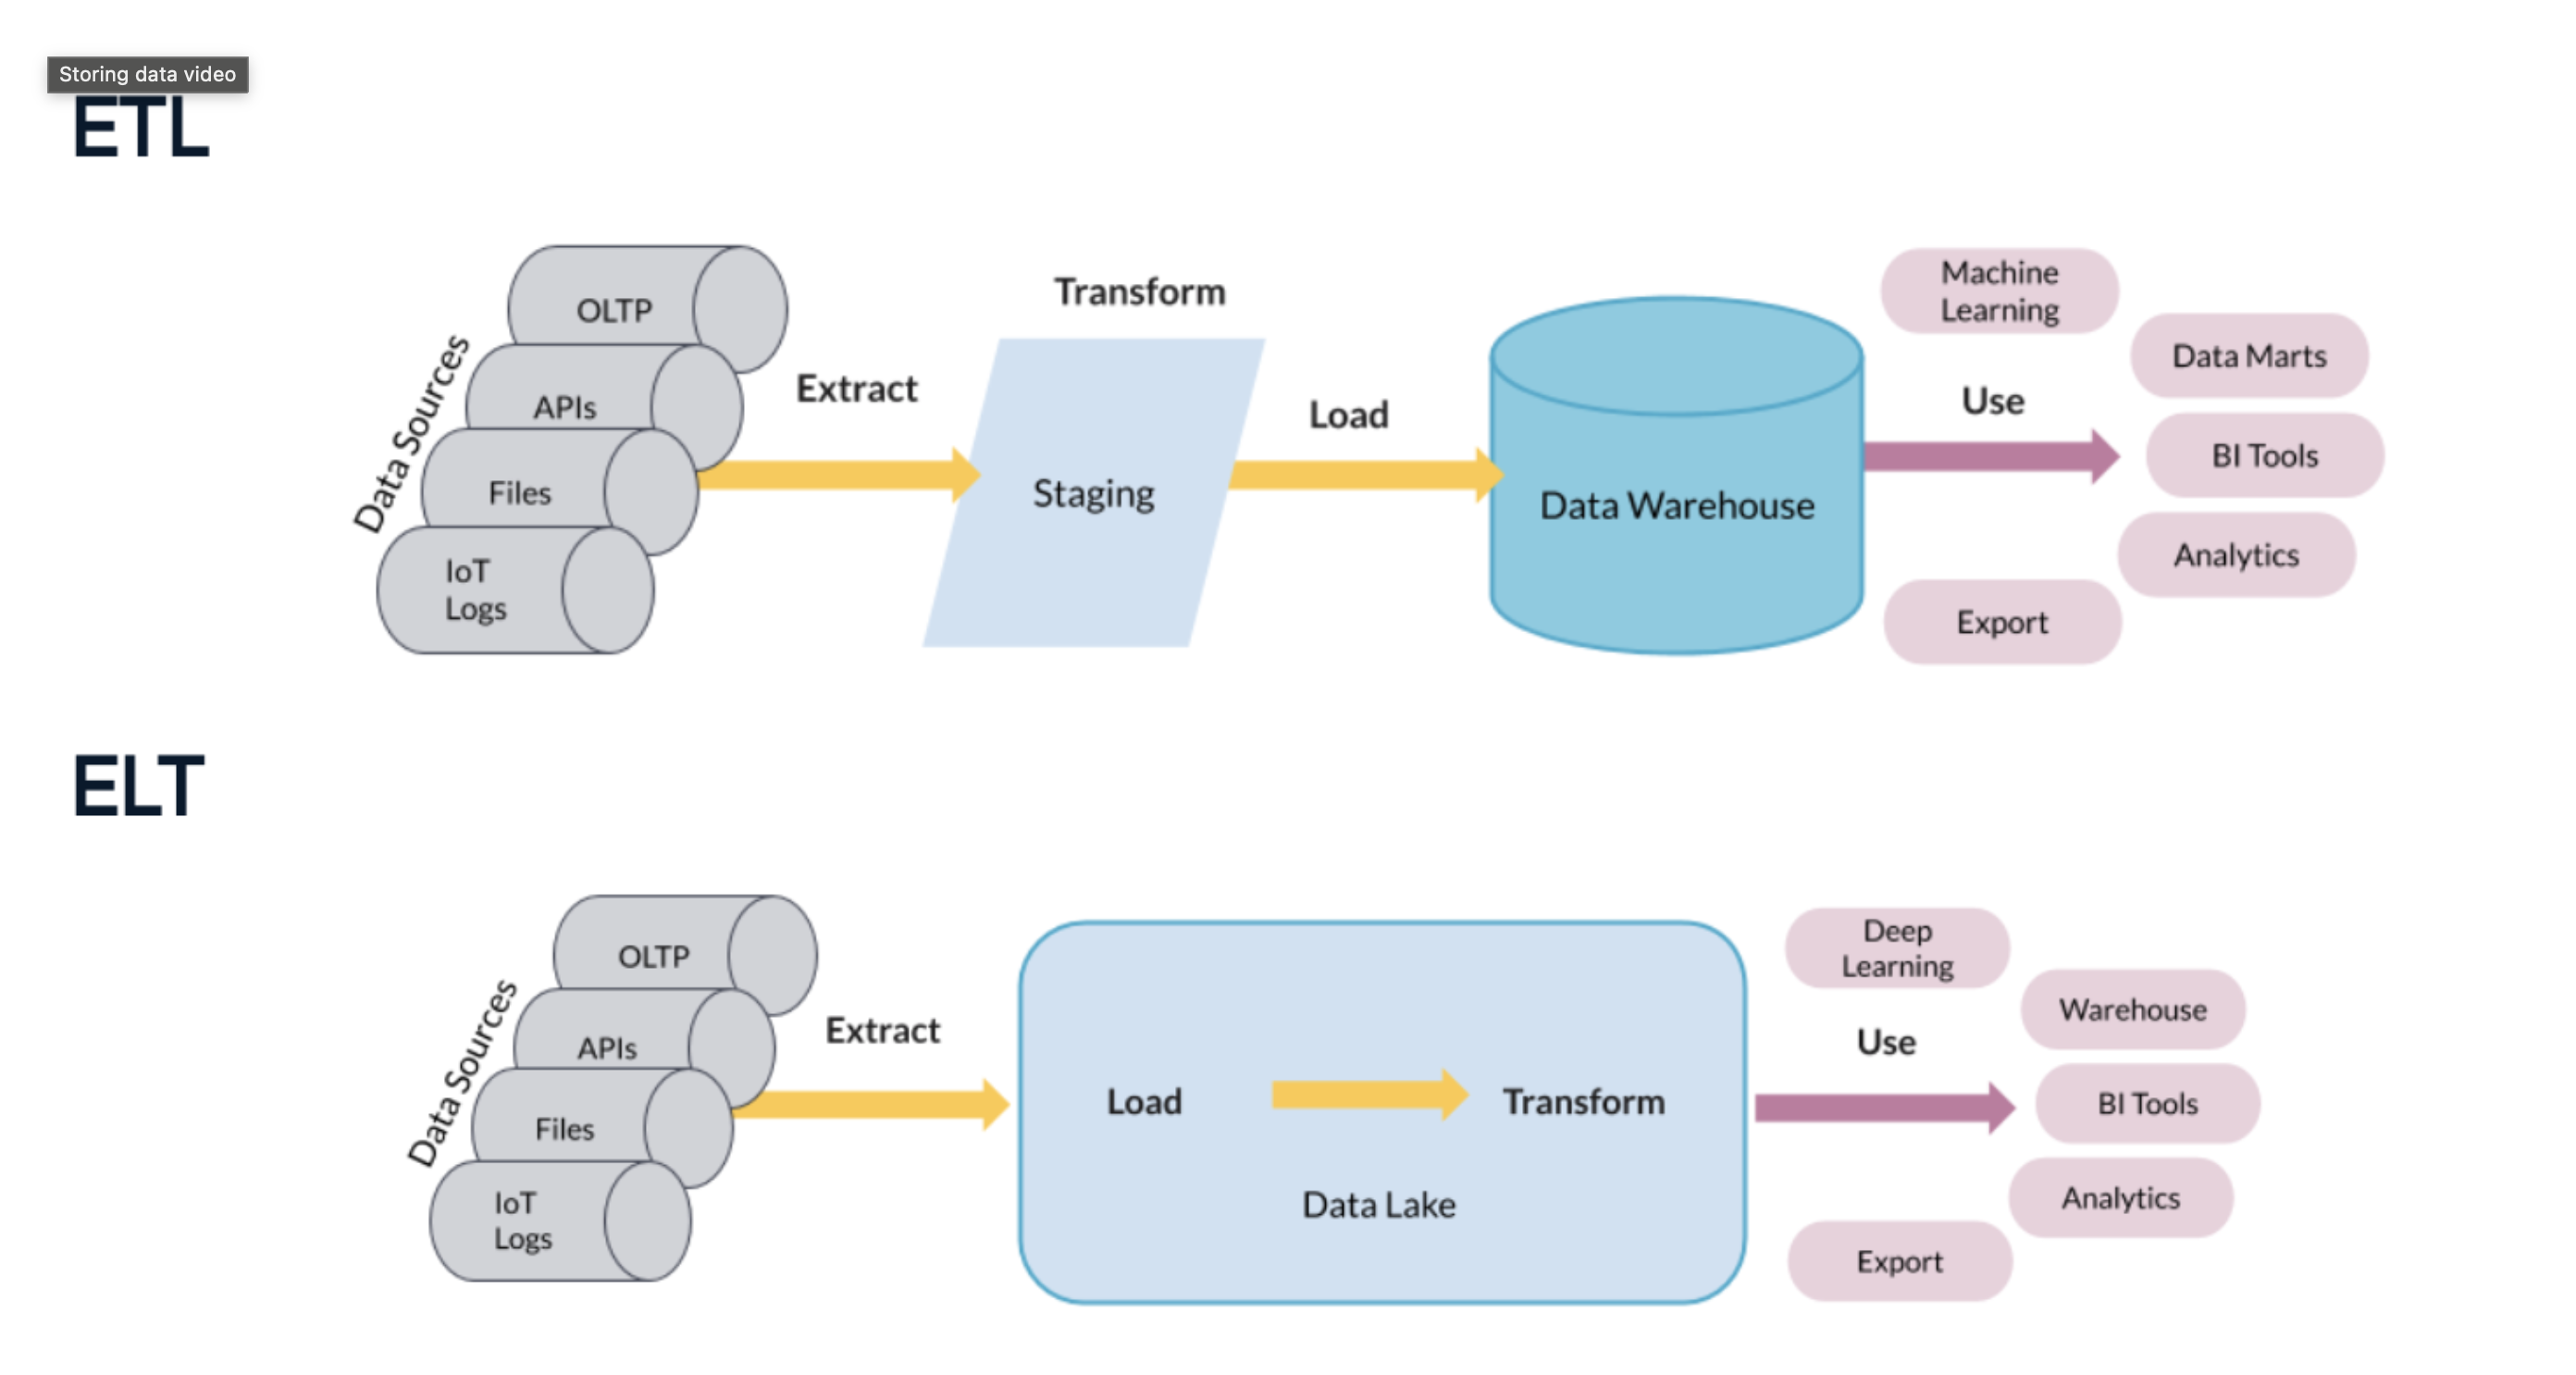
\includegraphics[width=1.0\textwidth]{figures/DataApproaches.png}
    \caption{Different Approaches in Data Flow}
    \label{fig:DataFlowApproaches}
\end{figure}

\subsection{Database Design}
\subsubsection{What is database design?}
\begin{itemize}
    \item Determines how data is logically stored.
    \begin{itemize}
        \item How is data going to be read and updated?
    \end{itemize}
    \item Uses \textbf{database models}: a high level specifications for database structure
    \begin{itemize}
        \item Most popular: relational model
        \item Some other options: NoSQL model, Object Oriented model, network model
    \end{itemize}
    \item Uses \textbf{schemas}: blueprint of the database
    \begin{itemize}
        \item Defines table, fields, relationships, indexes and Views
        \item When inserting data in relational databases, schema must be respected
    \end{itemize}
\end{itemize}

\subsubsection{Data modeling}
Process of creating a data model for the data to be stored.\\
Level of modeling
\begin{enumerate}
    \item \textbf{Conceptual data model}: describe entities, relationships, and attributes \\
    \emph{Tools:}data structure diagram, e.g., entity-relational diagrams and UML diagrams
    \item \textbf{Logical data model}: defines tables, columns, and relationships \\
    \emph{Tools:} database models and schemas, e.g., relational model and star Schema
    \item \textbf{Physical data model}: describes physical storage \\
    \emph{Tools:} partitions, CPUs, indexes, backup systems and tablespaces
\end{enumerate}

\begin{figure}[H]
    \centering
    \caption{Data Models}
    \label{fig:DataModels}
    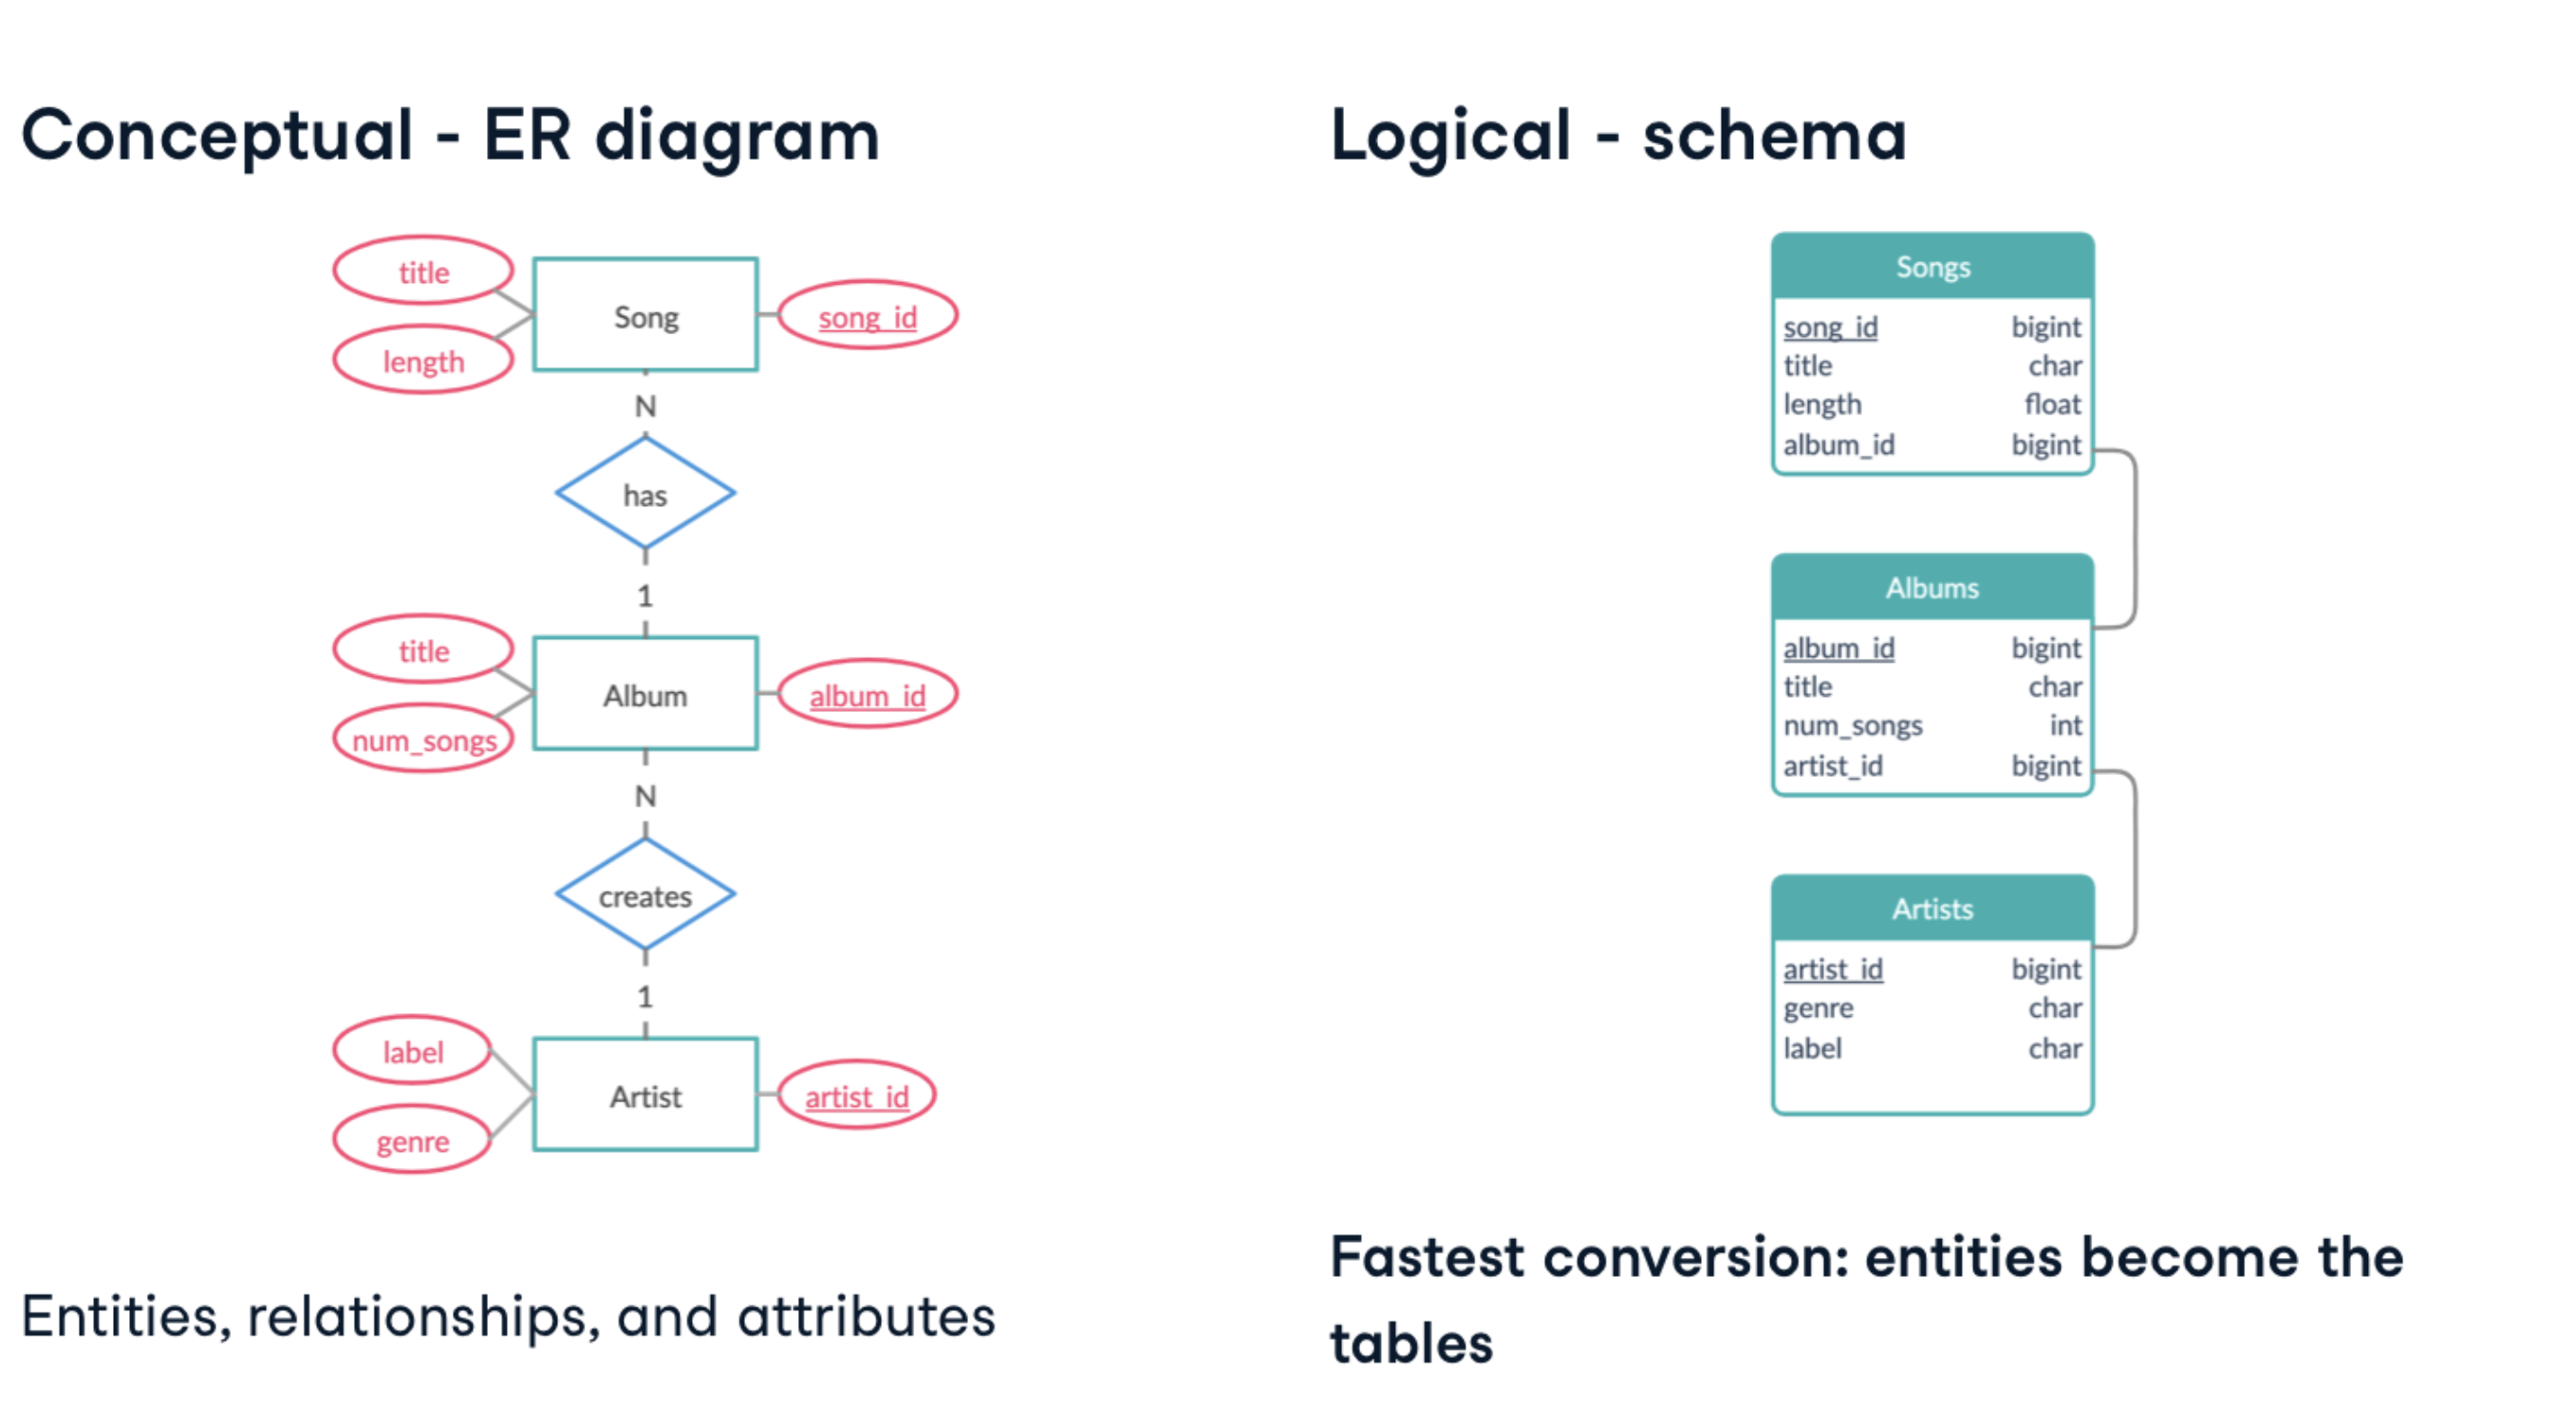
\includegraphics[width=1.0\textwidth]{figures/DataModels.png}
\end{figure}

\subsubsection{Beyond the relational model \\Dimensional modeling}
Adaptation of the relational model for data warehouse design
\begin{itemize}
    \item Optimized for \textbf{OLAP} queries: aggregate data, not updating (OLTP)
    \item Built using the star Schemas
    \item Easy to interpret and extend schema
\end{itemize}

\subsubsection{Elements of dimensional modeling}
\begin{figure}[H]
    \centering
    \caption{Elements of dimensional modeling}
    \label{fig:DimensionalModeling}
    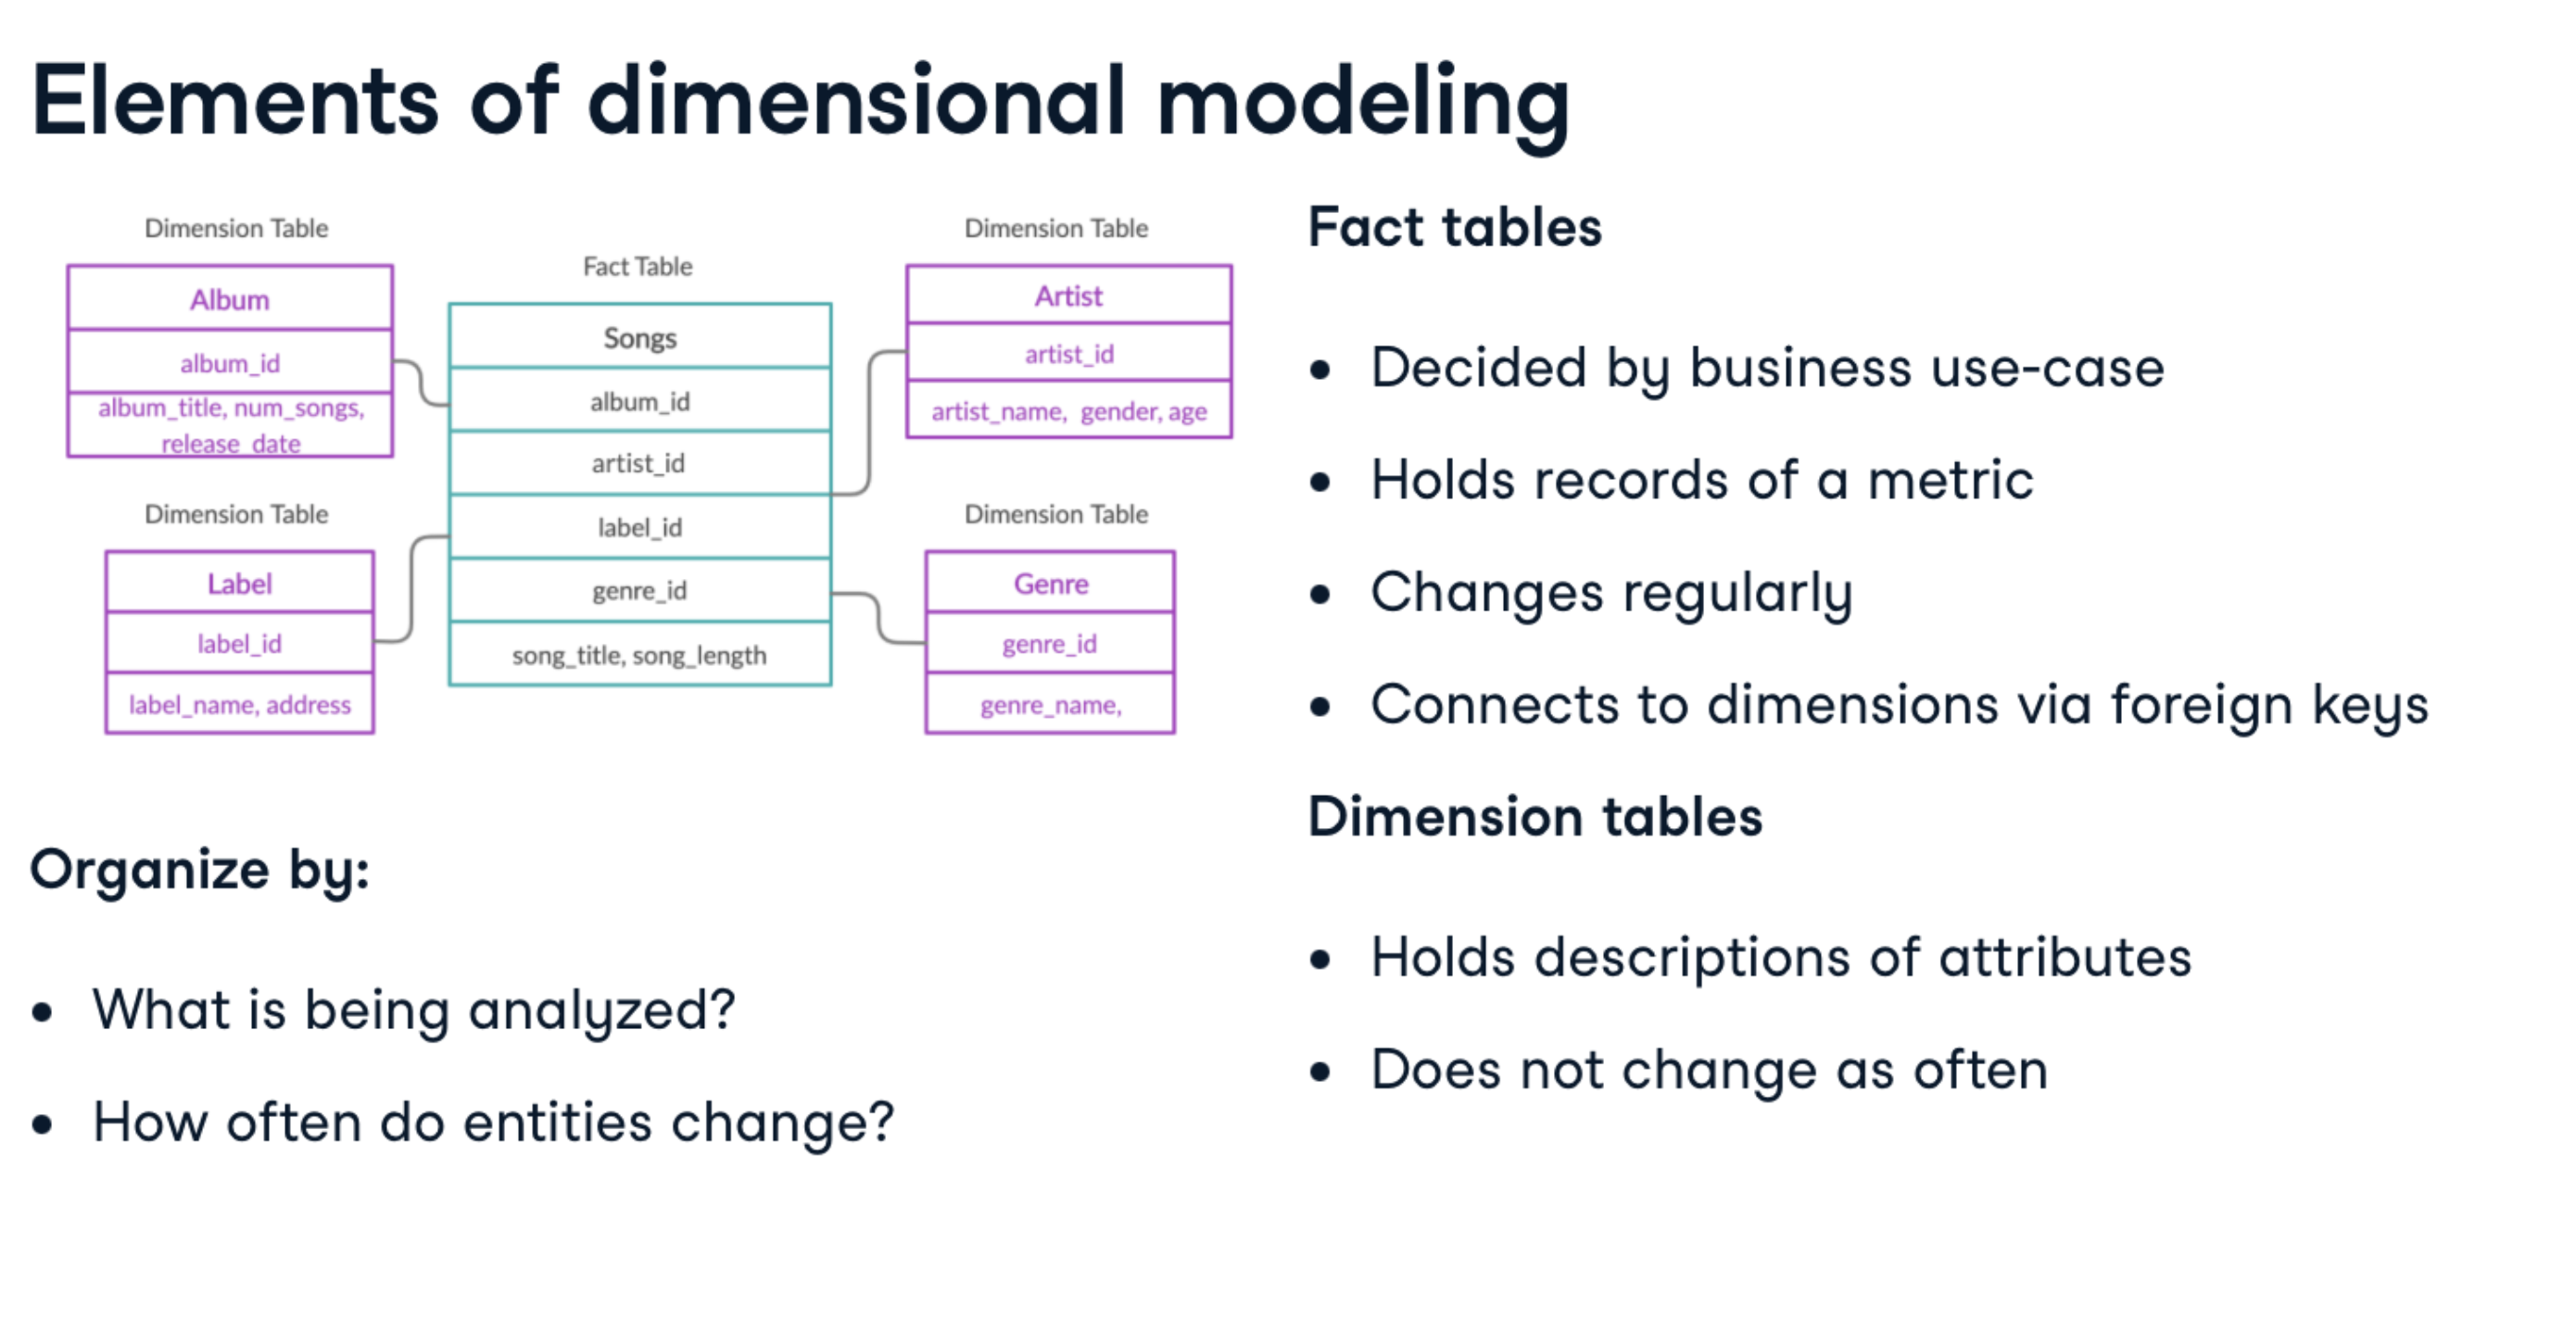
\includegraphics[width=1.0\textwidth]{figures/DimensionalModeling.png}
\end{figure}

\section{Database Schema and Normalization}
\subsection{Star and snowflake schema}
\subsubsection{Star schema}
\textbf{Dimensional modeling: star Schemas\\
Fact tables}
\begin{itemize}
    \item Holds records of metric
    \item Changes regularly
    \item Connects to dimensions via foreign keys
\end{itemize}
\textbf{Dimension tables}
\begin{itemize}
    \item Holds descriptions of attributes
    \item Does not change as often
\end{itemize}
\textbf{Example}
\begin{itemize}
    \item Supply books to stores in USA and Canada
    \item Keep track of book sales
\end{itemize}

\begin{figure}[H]
    \centering
    \caption{Example of Star Schema}
    \label{fig:StarSchemaExample}
    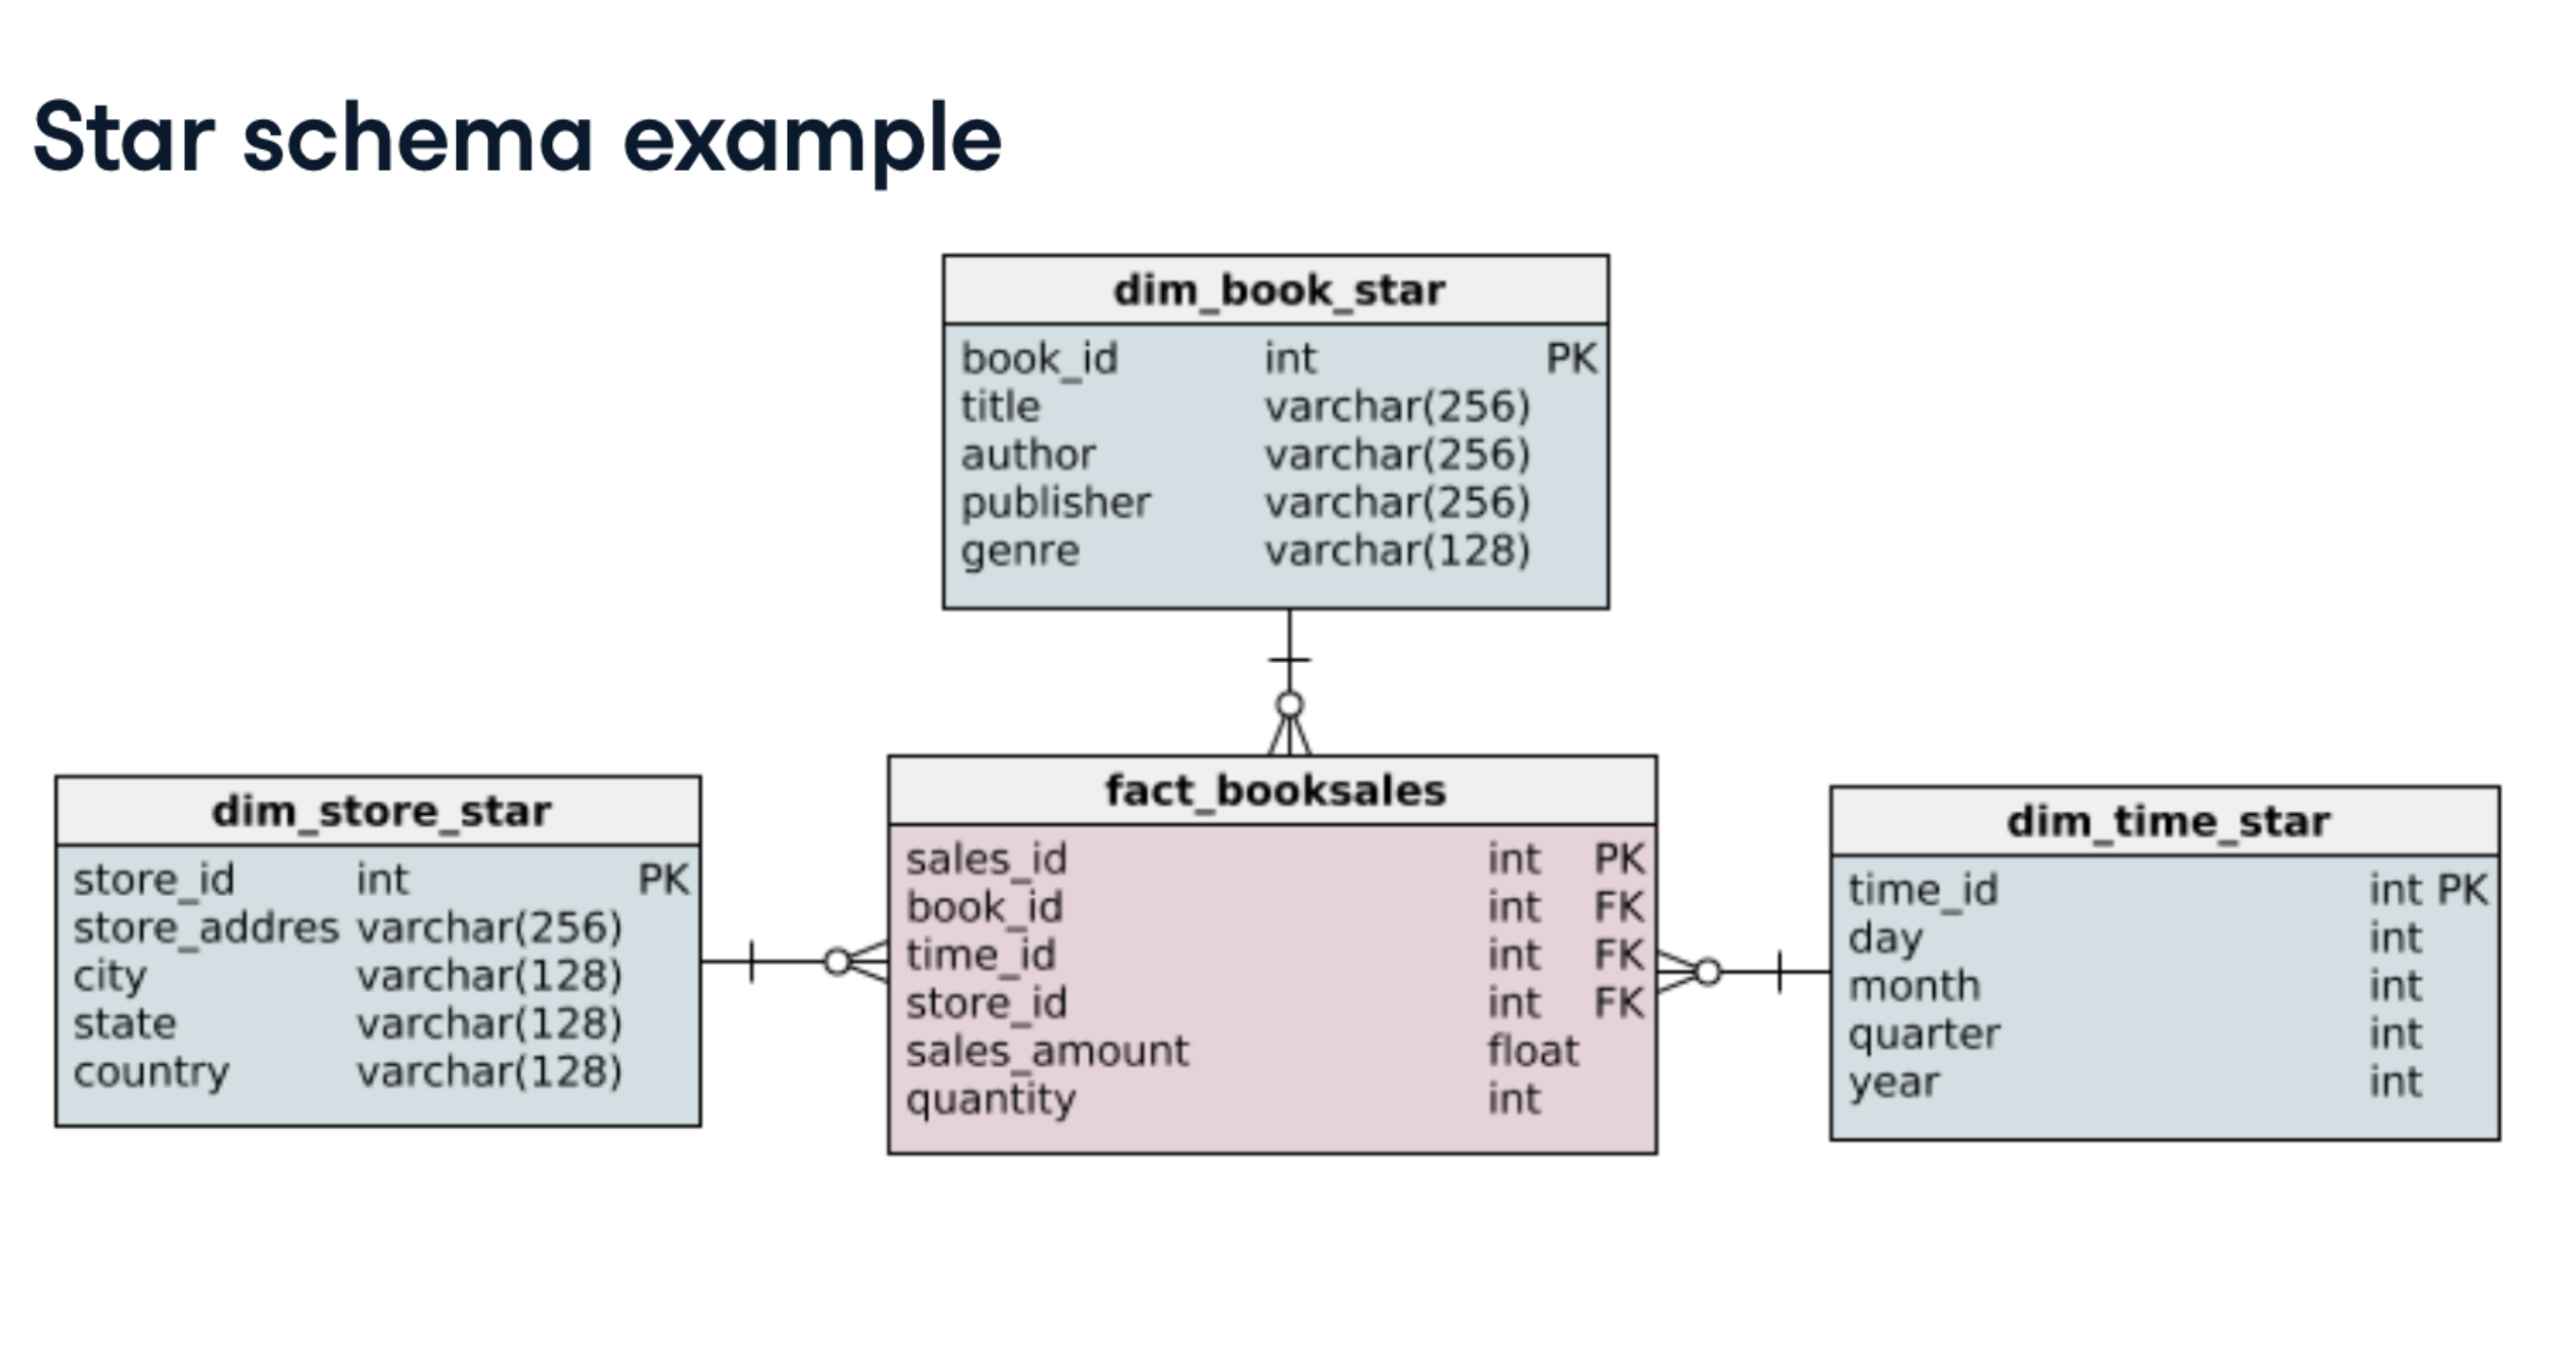
\includegraphics[width=1.0\textwidth]{figures/StarSchemaExample.png}
\end{figure}

Snowflake Schema is just an extension of Star schema where fact table remain 
same but dimension tables are further Normalized.
\begin{figure}[H]
    \centering
    \caption{Example of SnowflakeSchema}
    \label{fig:SnowflakeSchema}
    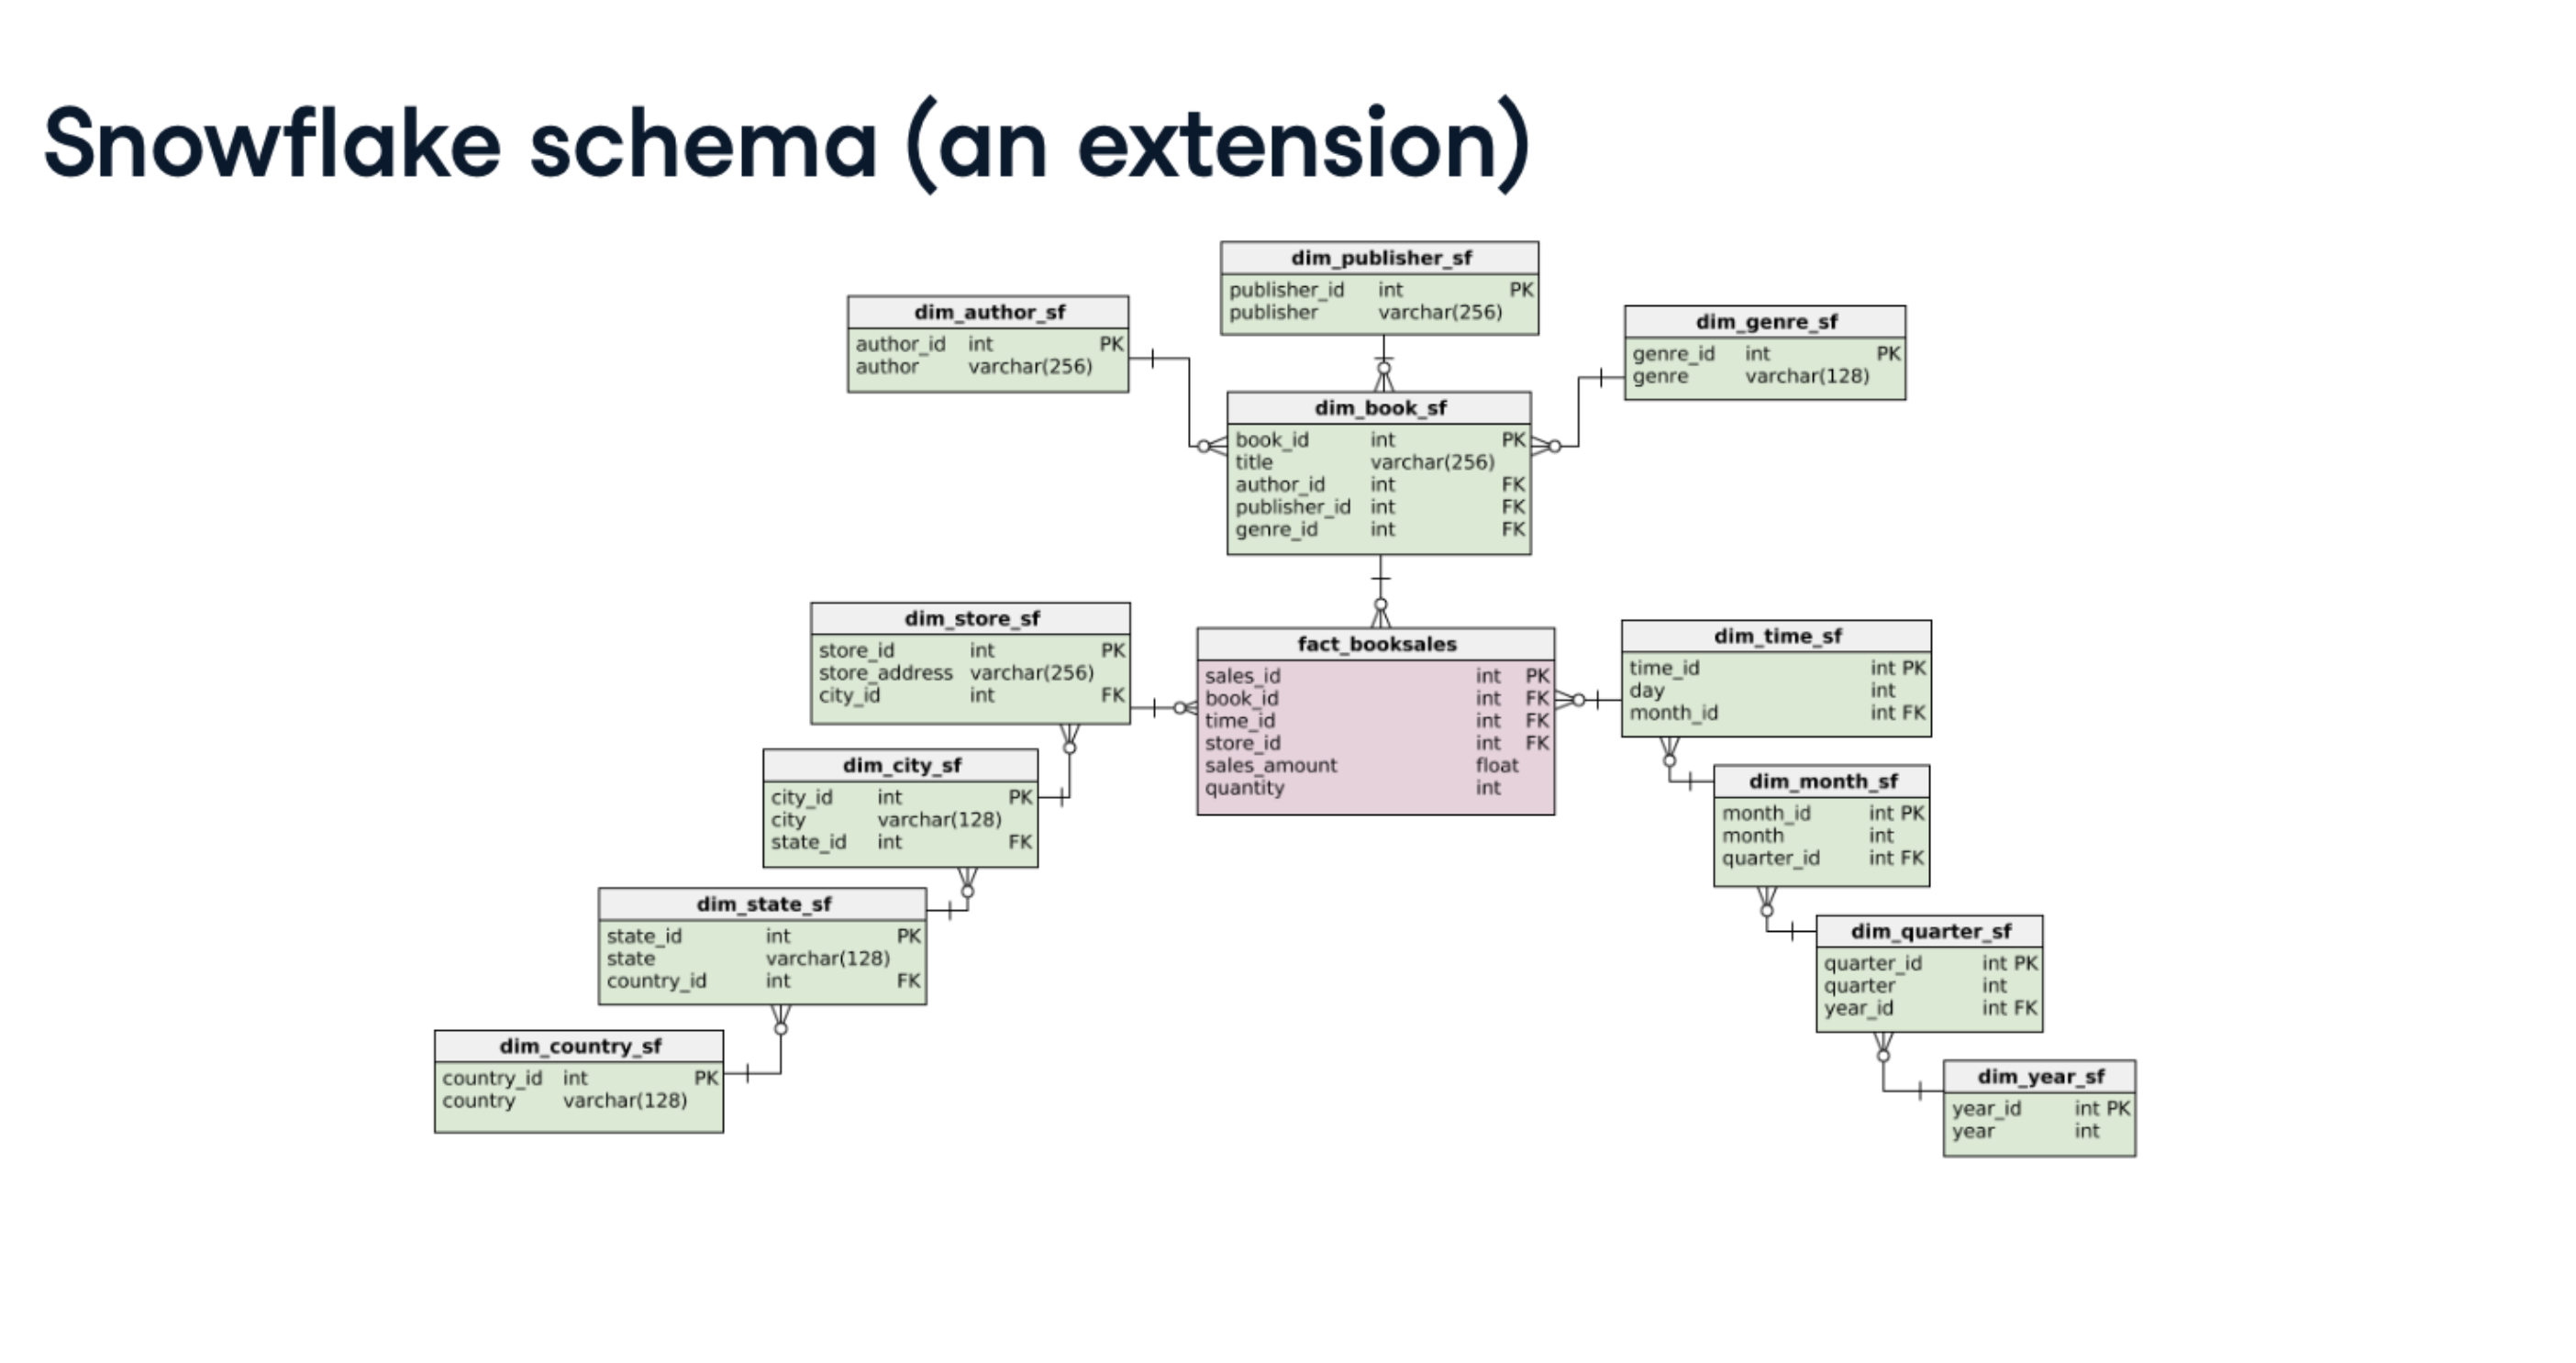
\includegraphics[width=1.0\textwidth]{figures/SnowflakeSchema.png}
\end{figure}

\begin{figure}[H]
    \centering
    \caption{Difference in Star and SnowflakeSchema}
    \label{fig:SchemaDifference}
    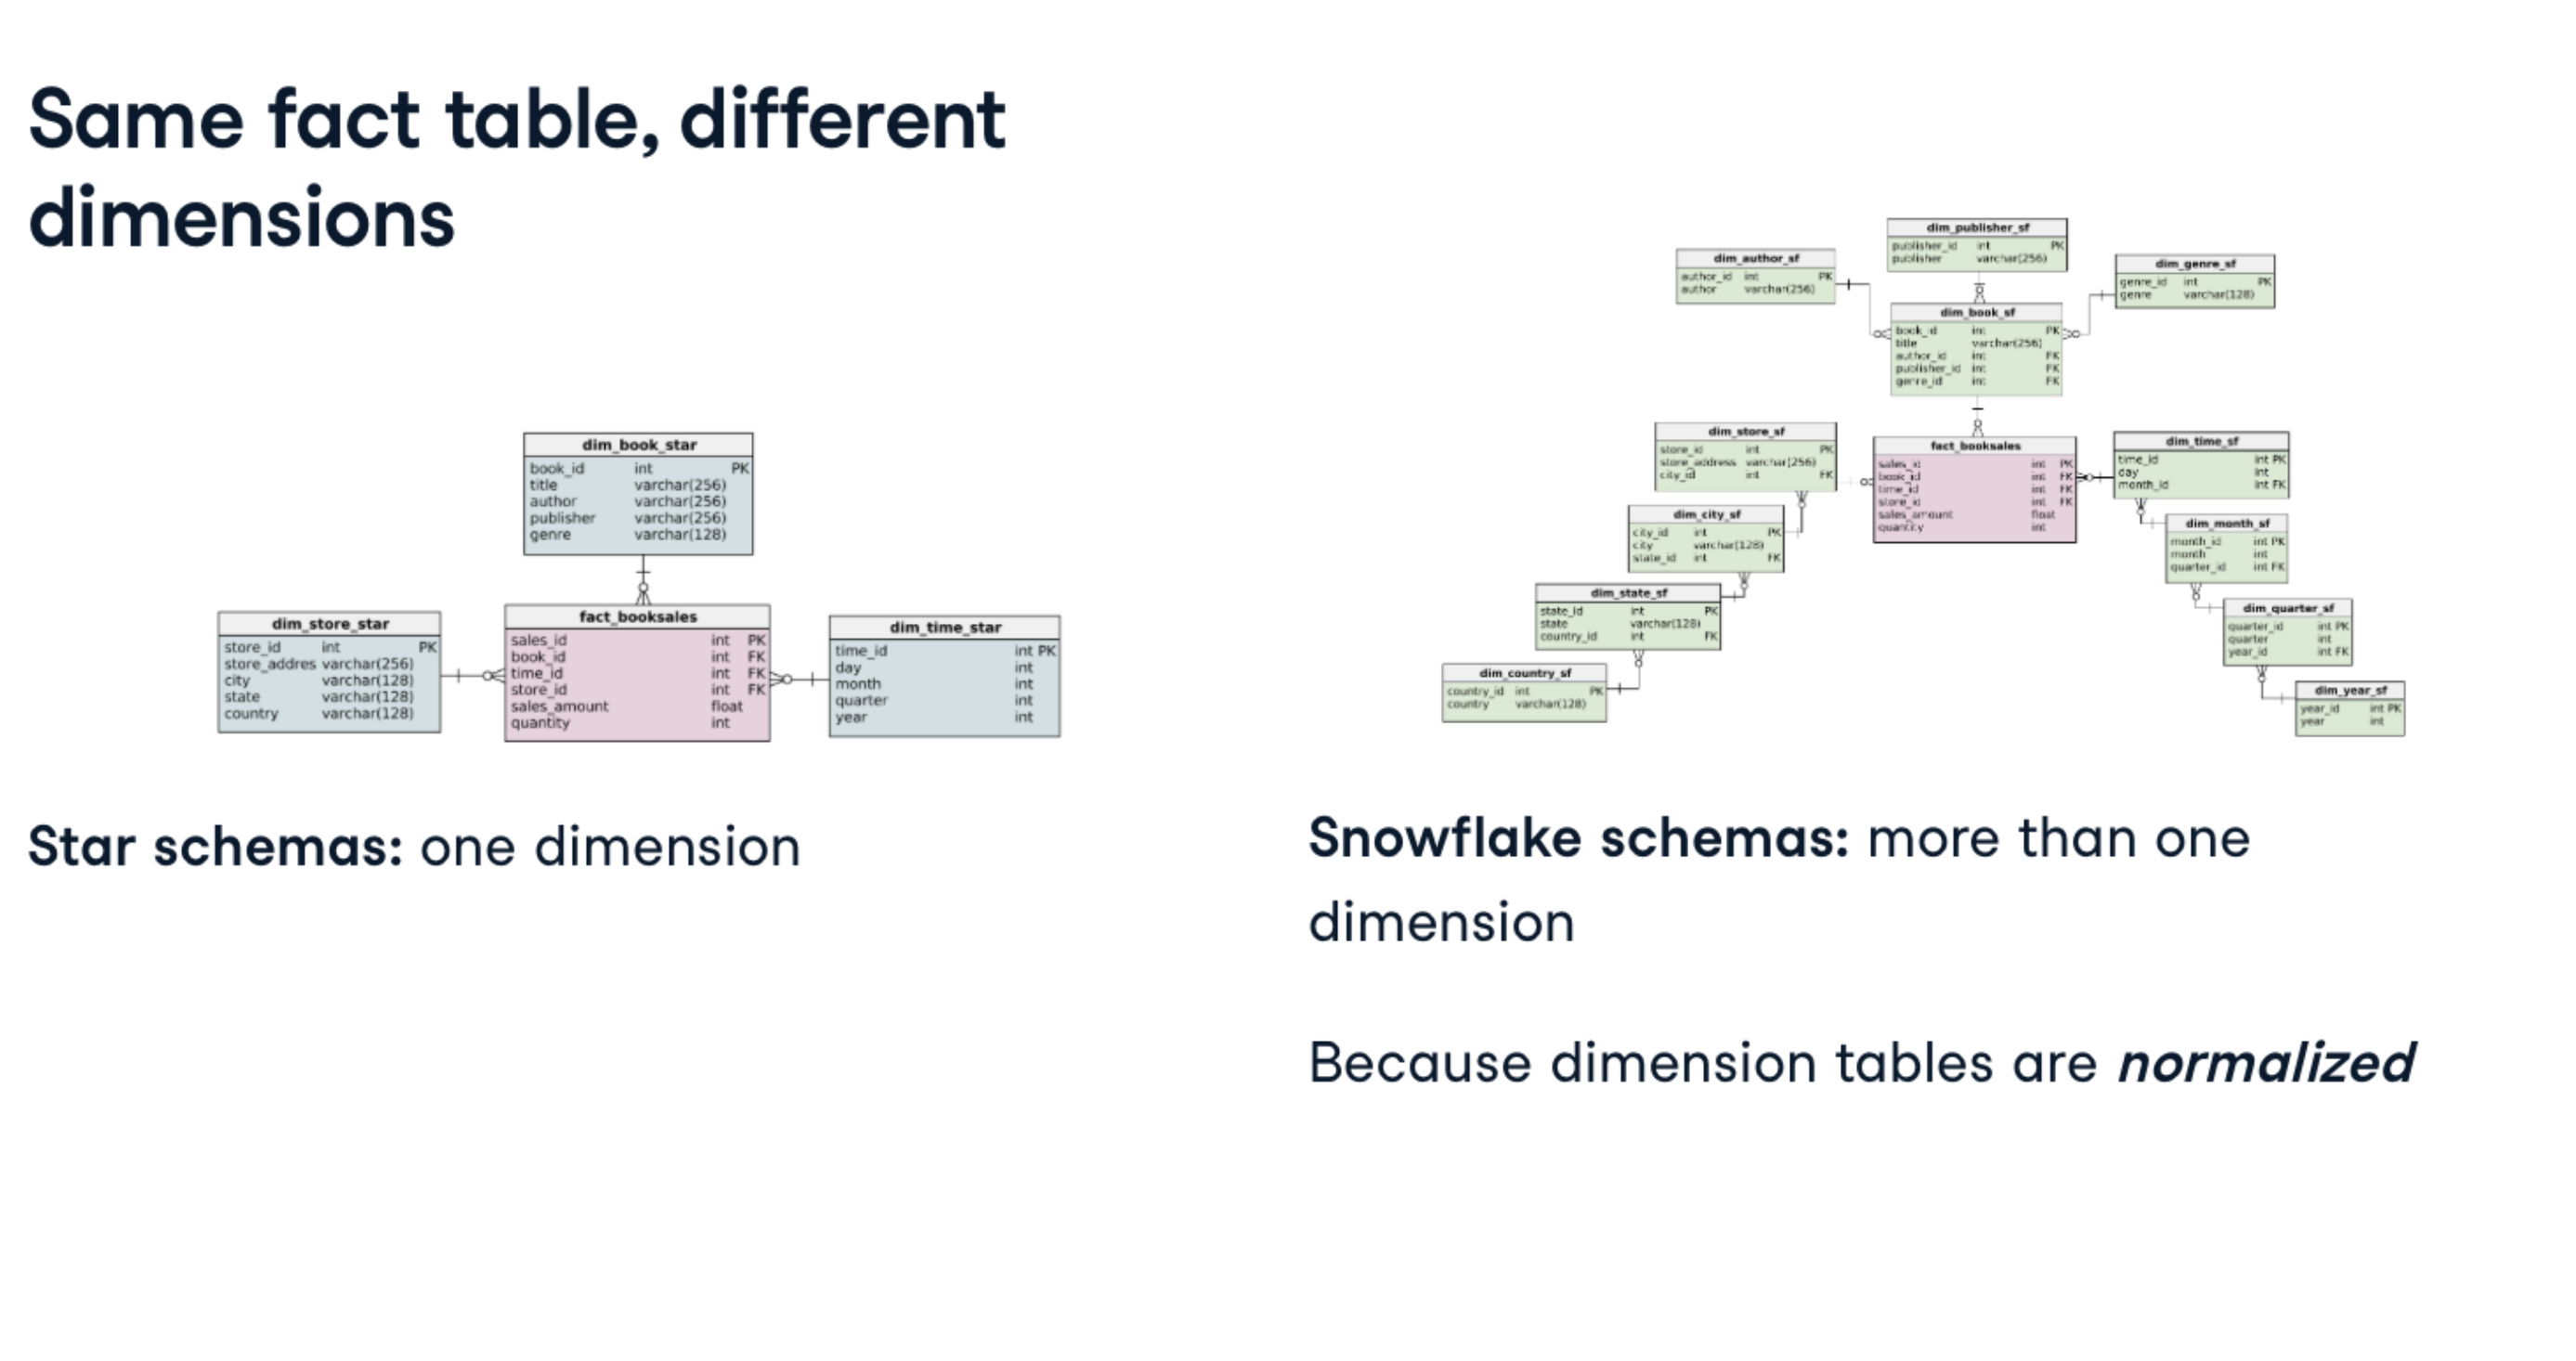
\includegraphics[width=1.0\textwidth]{figures/SchemaDifference.png}
\end{figure}

\subsubsection{What is Normalization?}
\begin{itemize}
    \item Database Design Technique
    \item Divide tables into smaller tables and connect them via relationships
    \item \textbf{Goal}: Reduce redundency and increase data integrity
\end{itemize}
\textbf{\emph{Identify repeating groups of data and create new tables for them}}

\begin{figure}[H]
    \centering
    \caption{Book Dimension}
    \label{fig:BookDimension}
    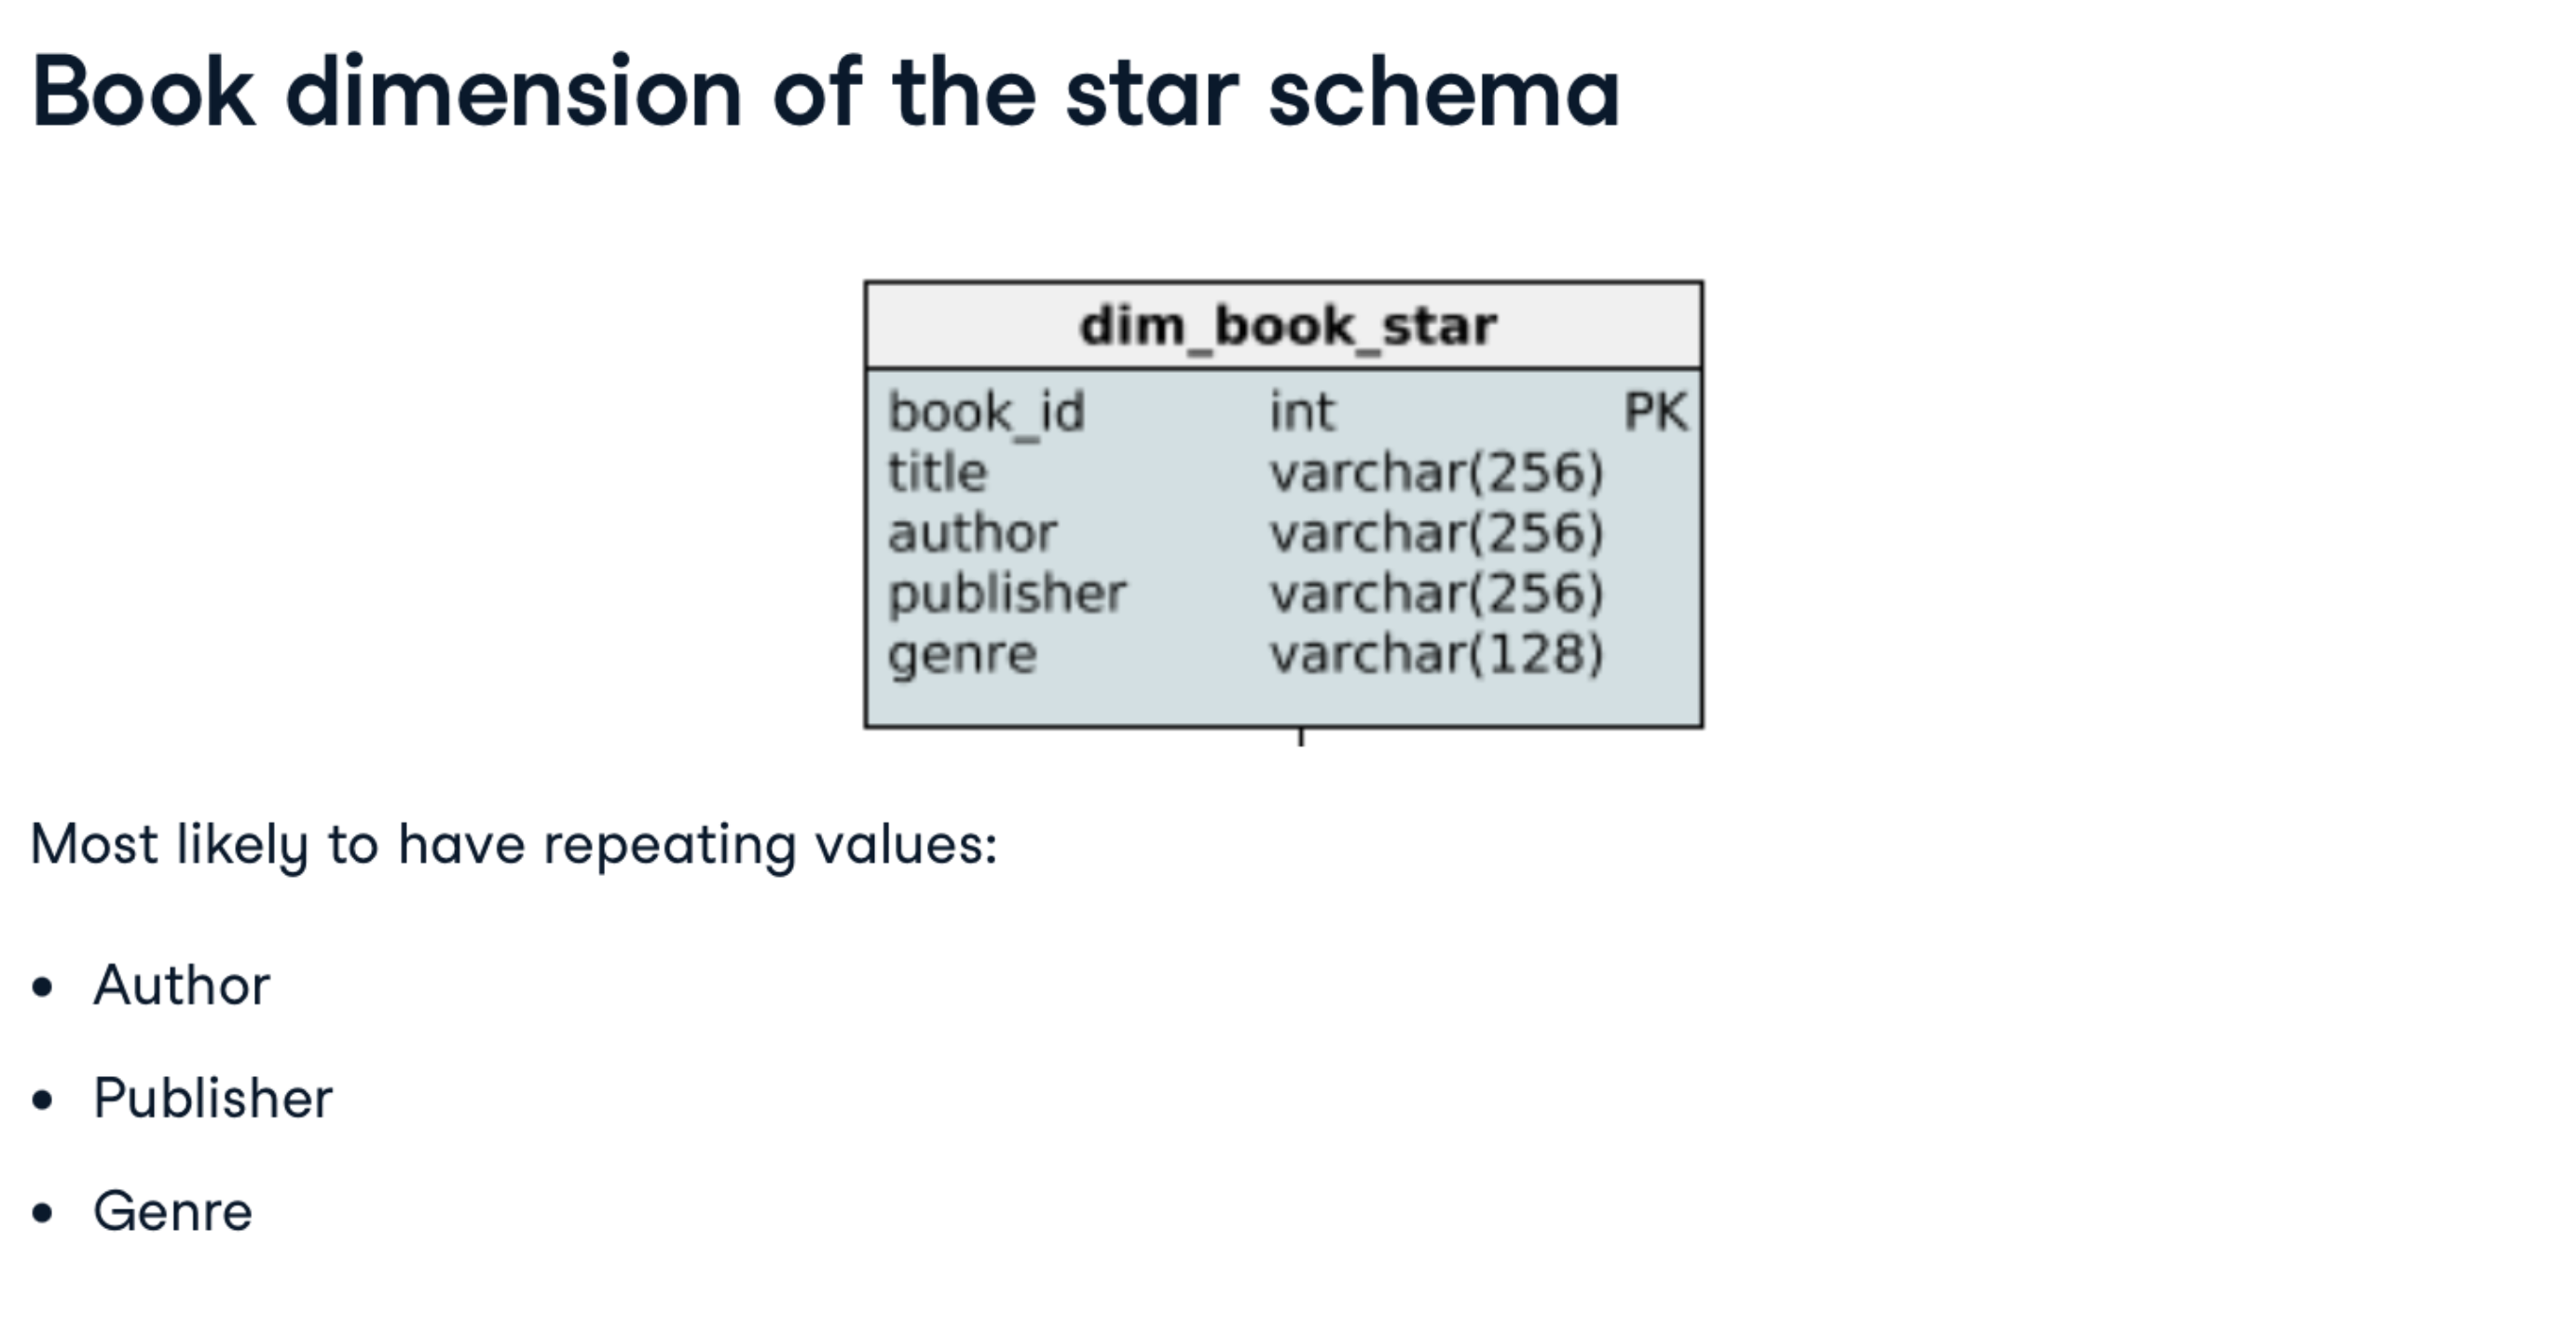
\includegraphics[width=1.0\textwidth]{figures/BookDimension.png}
\end{figure}

\begin{figure}[H]
    \centering
    \caption{Extension of Book Dimension}
    \label{fig:BookDimensionExtended}
    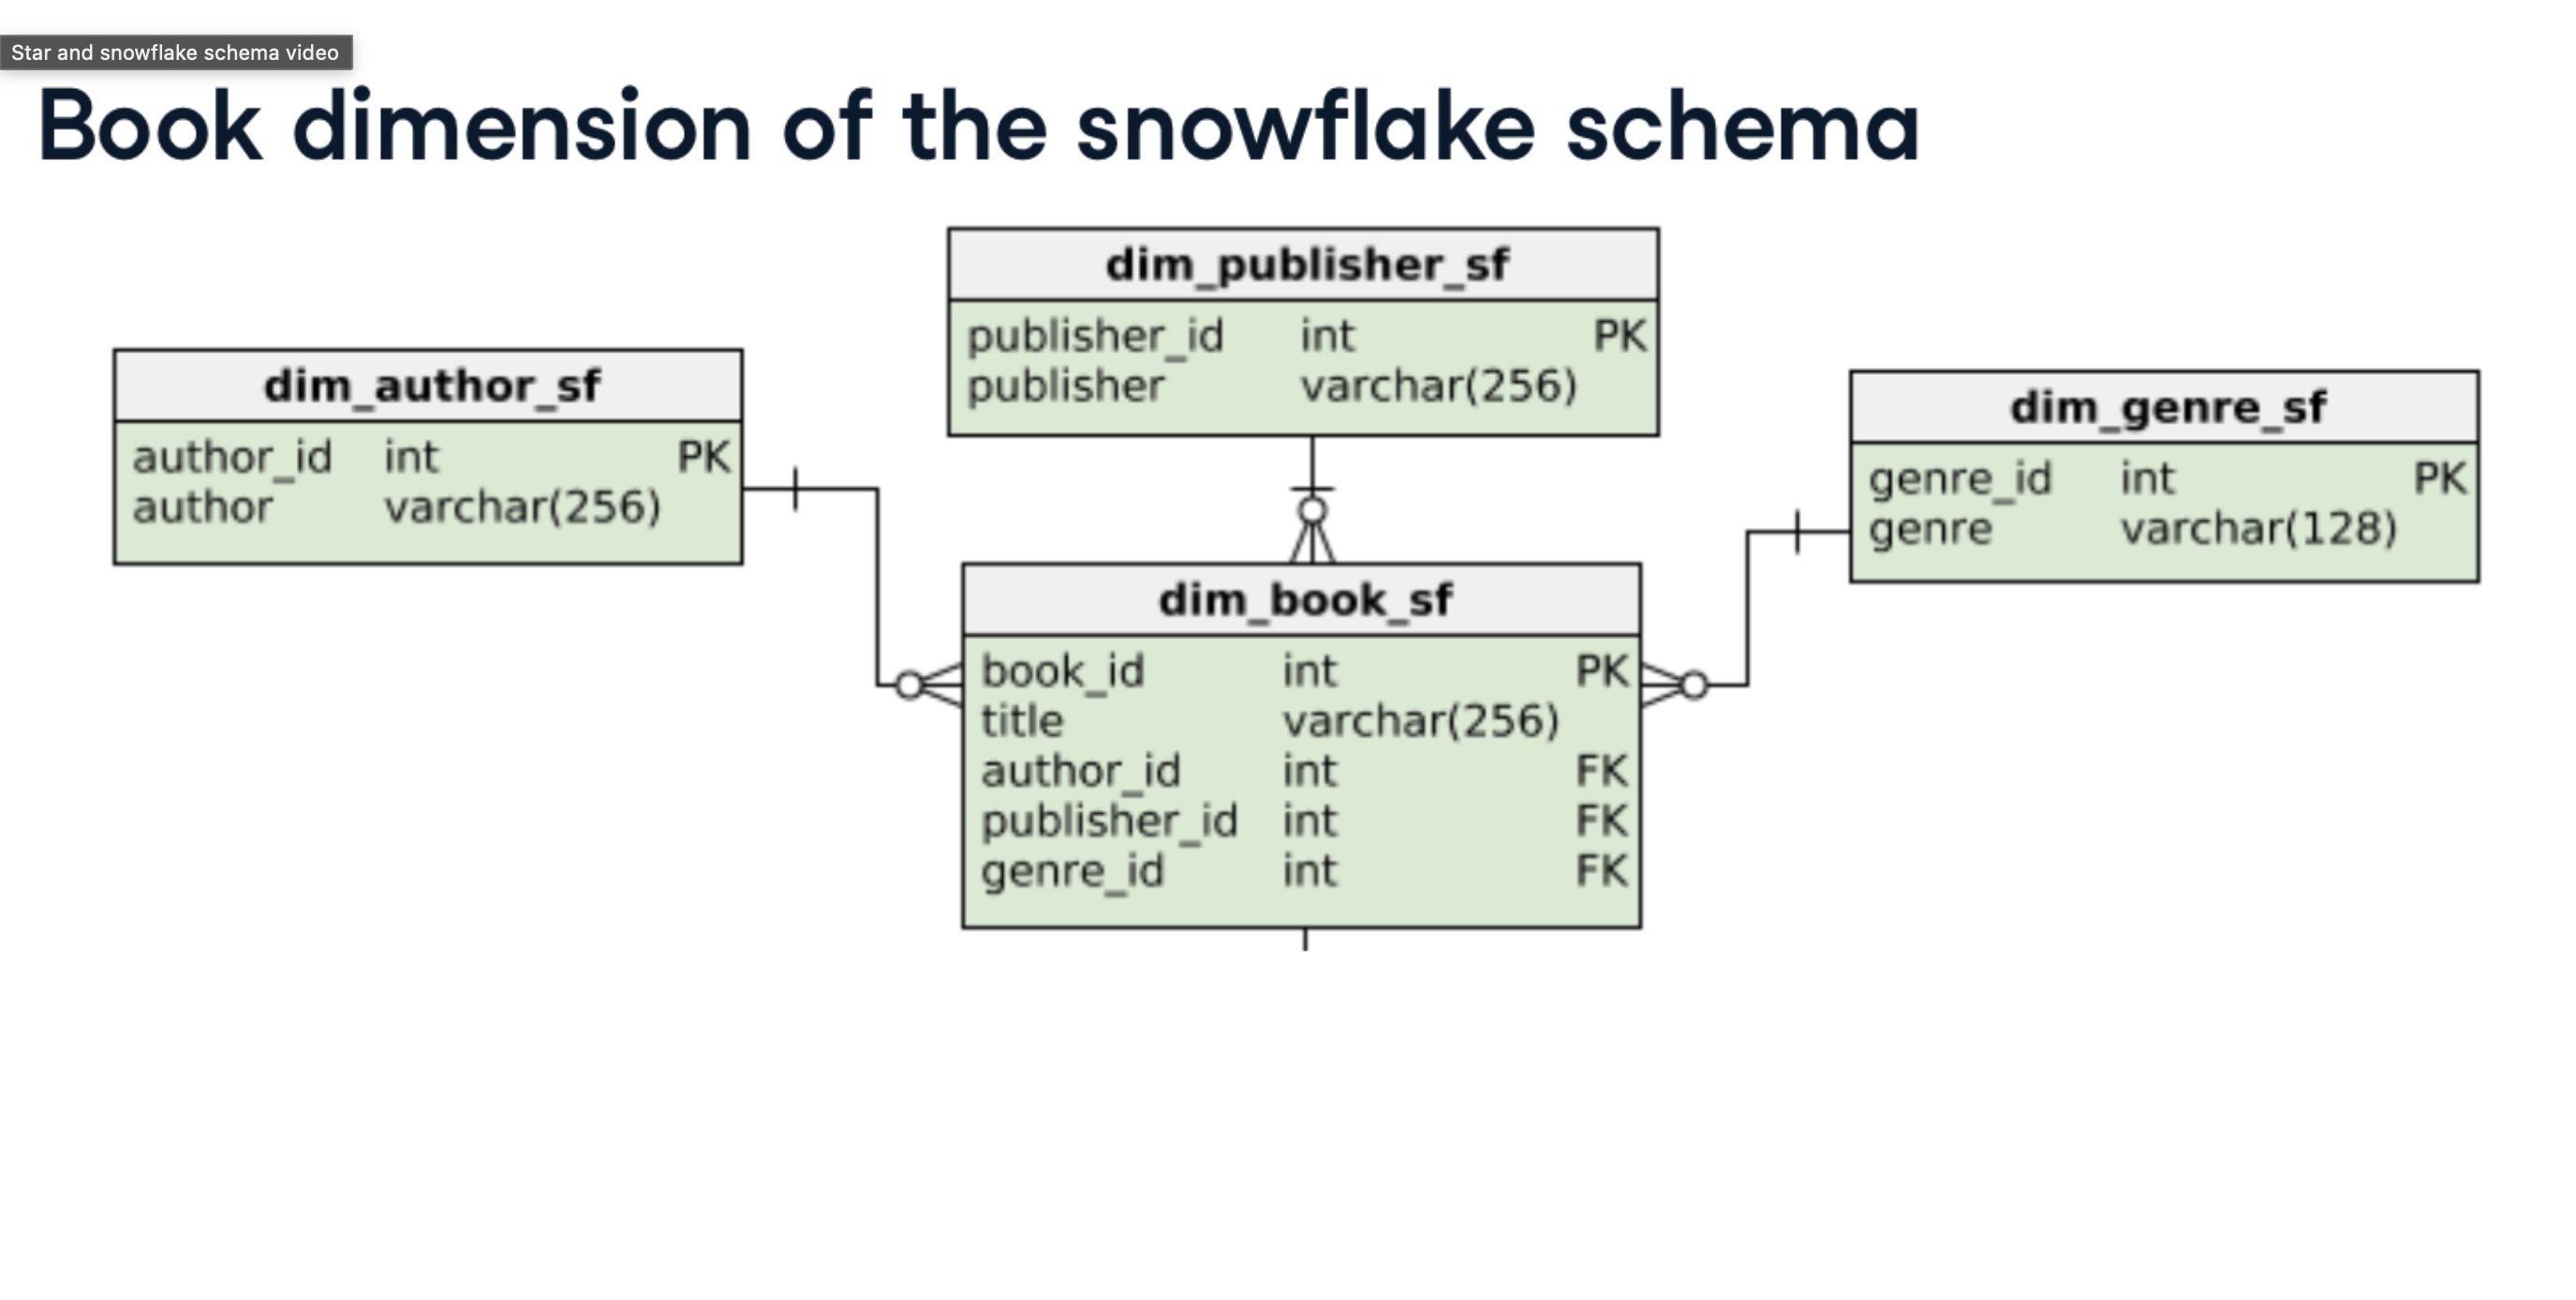
\includegraphics[width=1.0\textwidth]{figures/BookDimensionExtended.png}
\end{figure}


\begin{figure}[H]
    \centering
    \caption{Store Dimension}
    \label{fig:StoreDimension}
    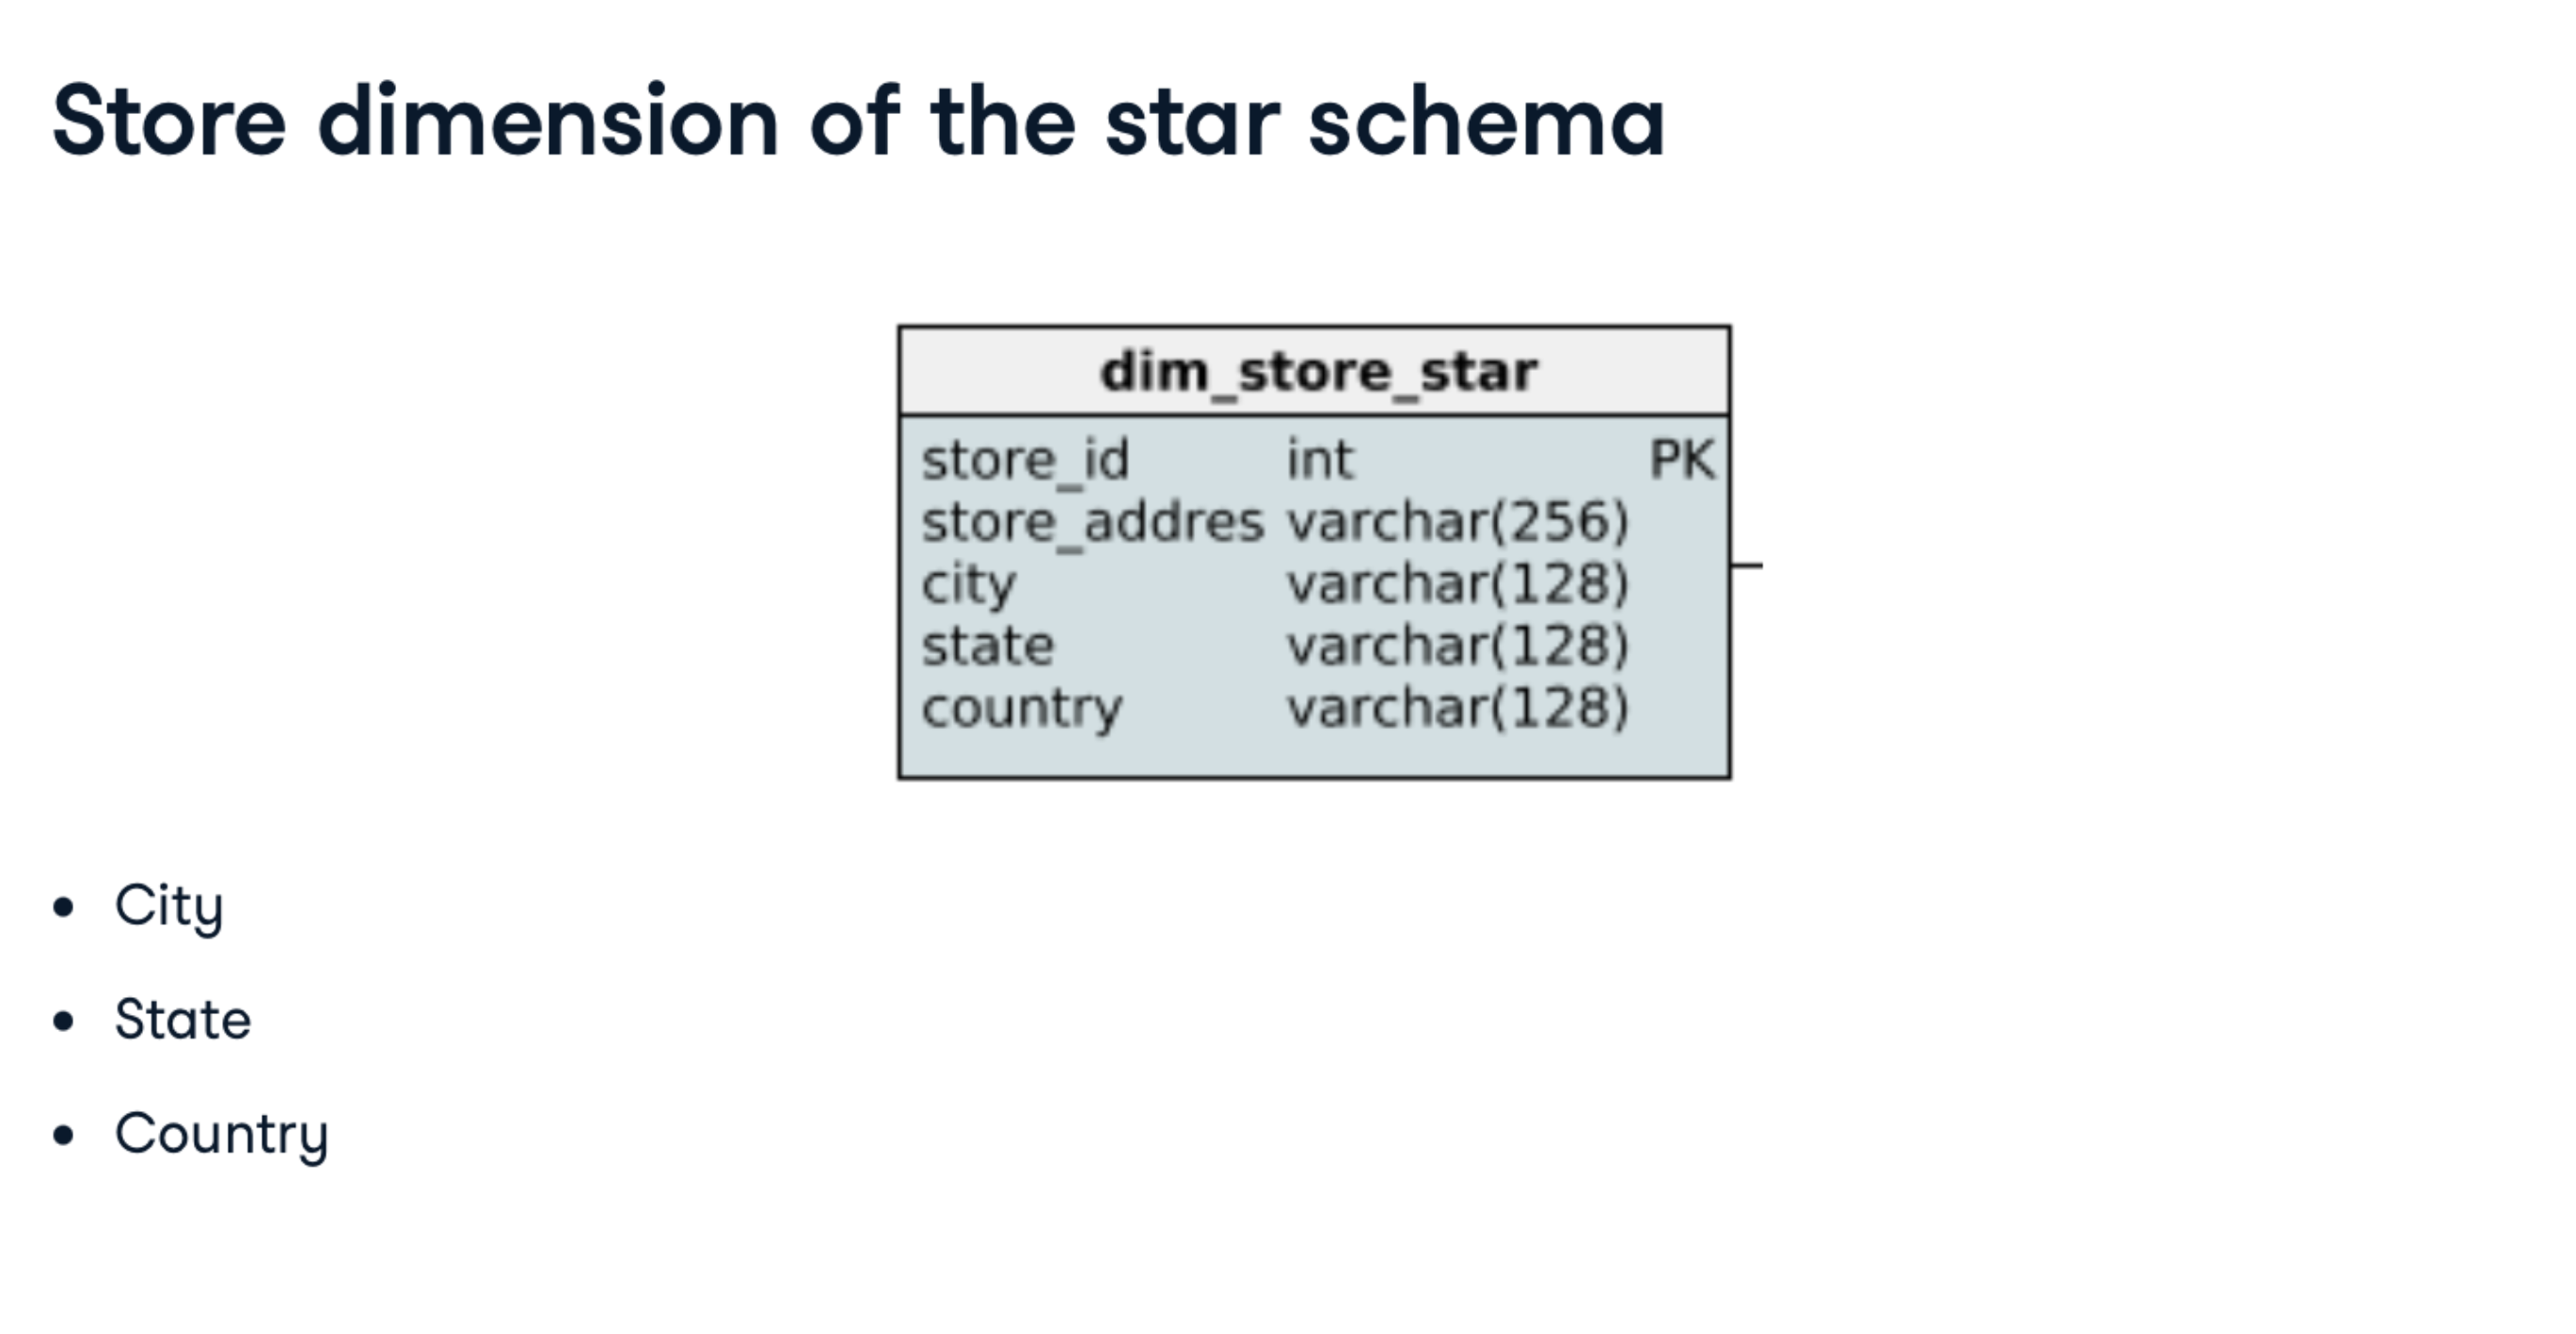
\includegraphics[width=1.0\textwidth]{figures/StoreDimension.png}
\end{figure}

\begin{figure}[H]
    \centering
    \caption{Extension of Store Dimension}
    \label{fig:StoreDimensionExtended}
    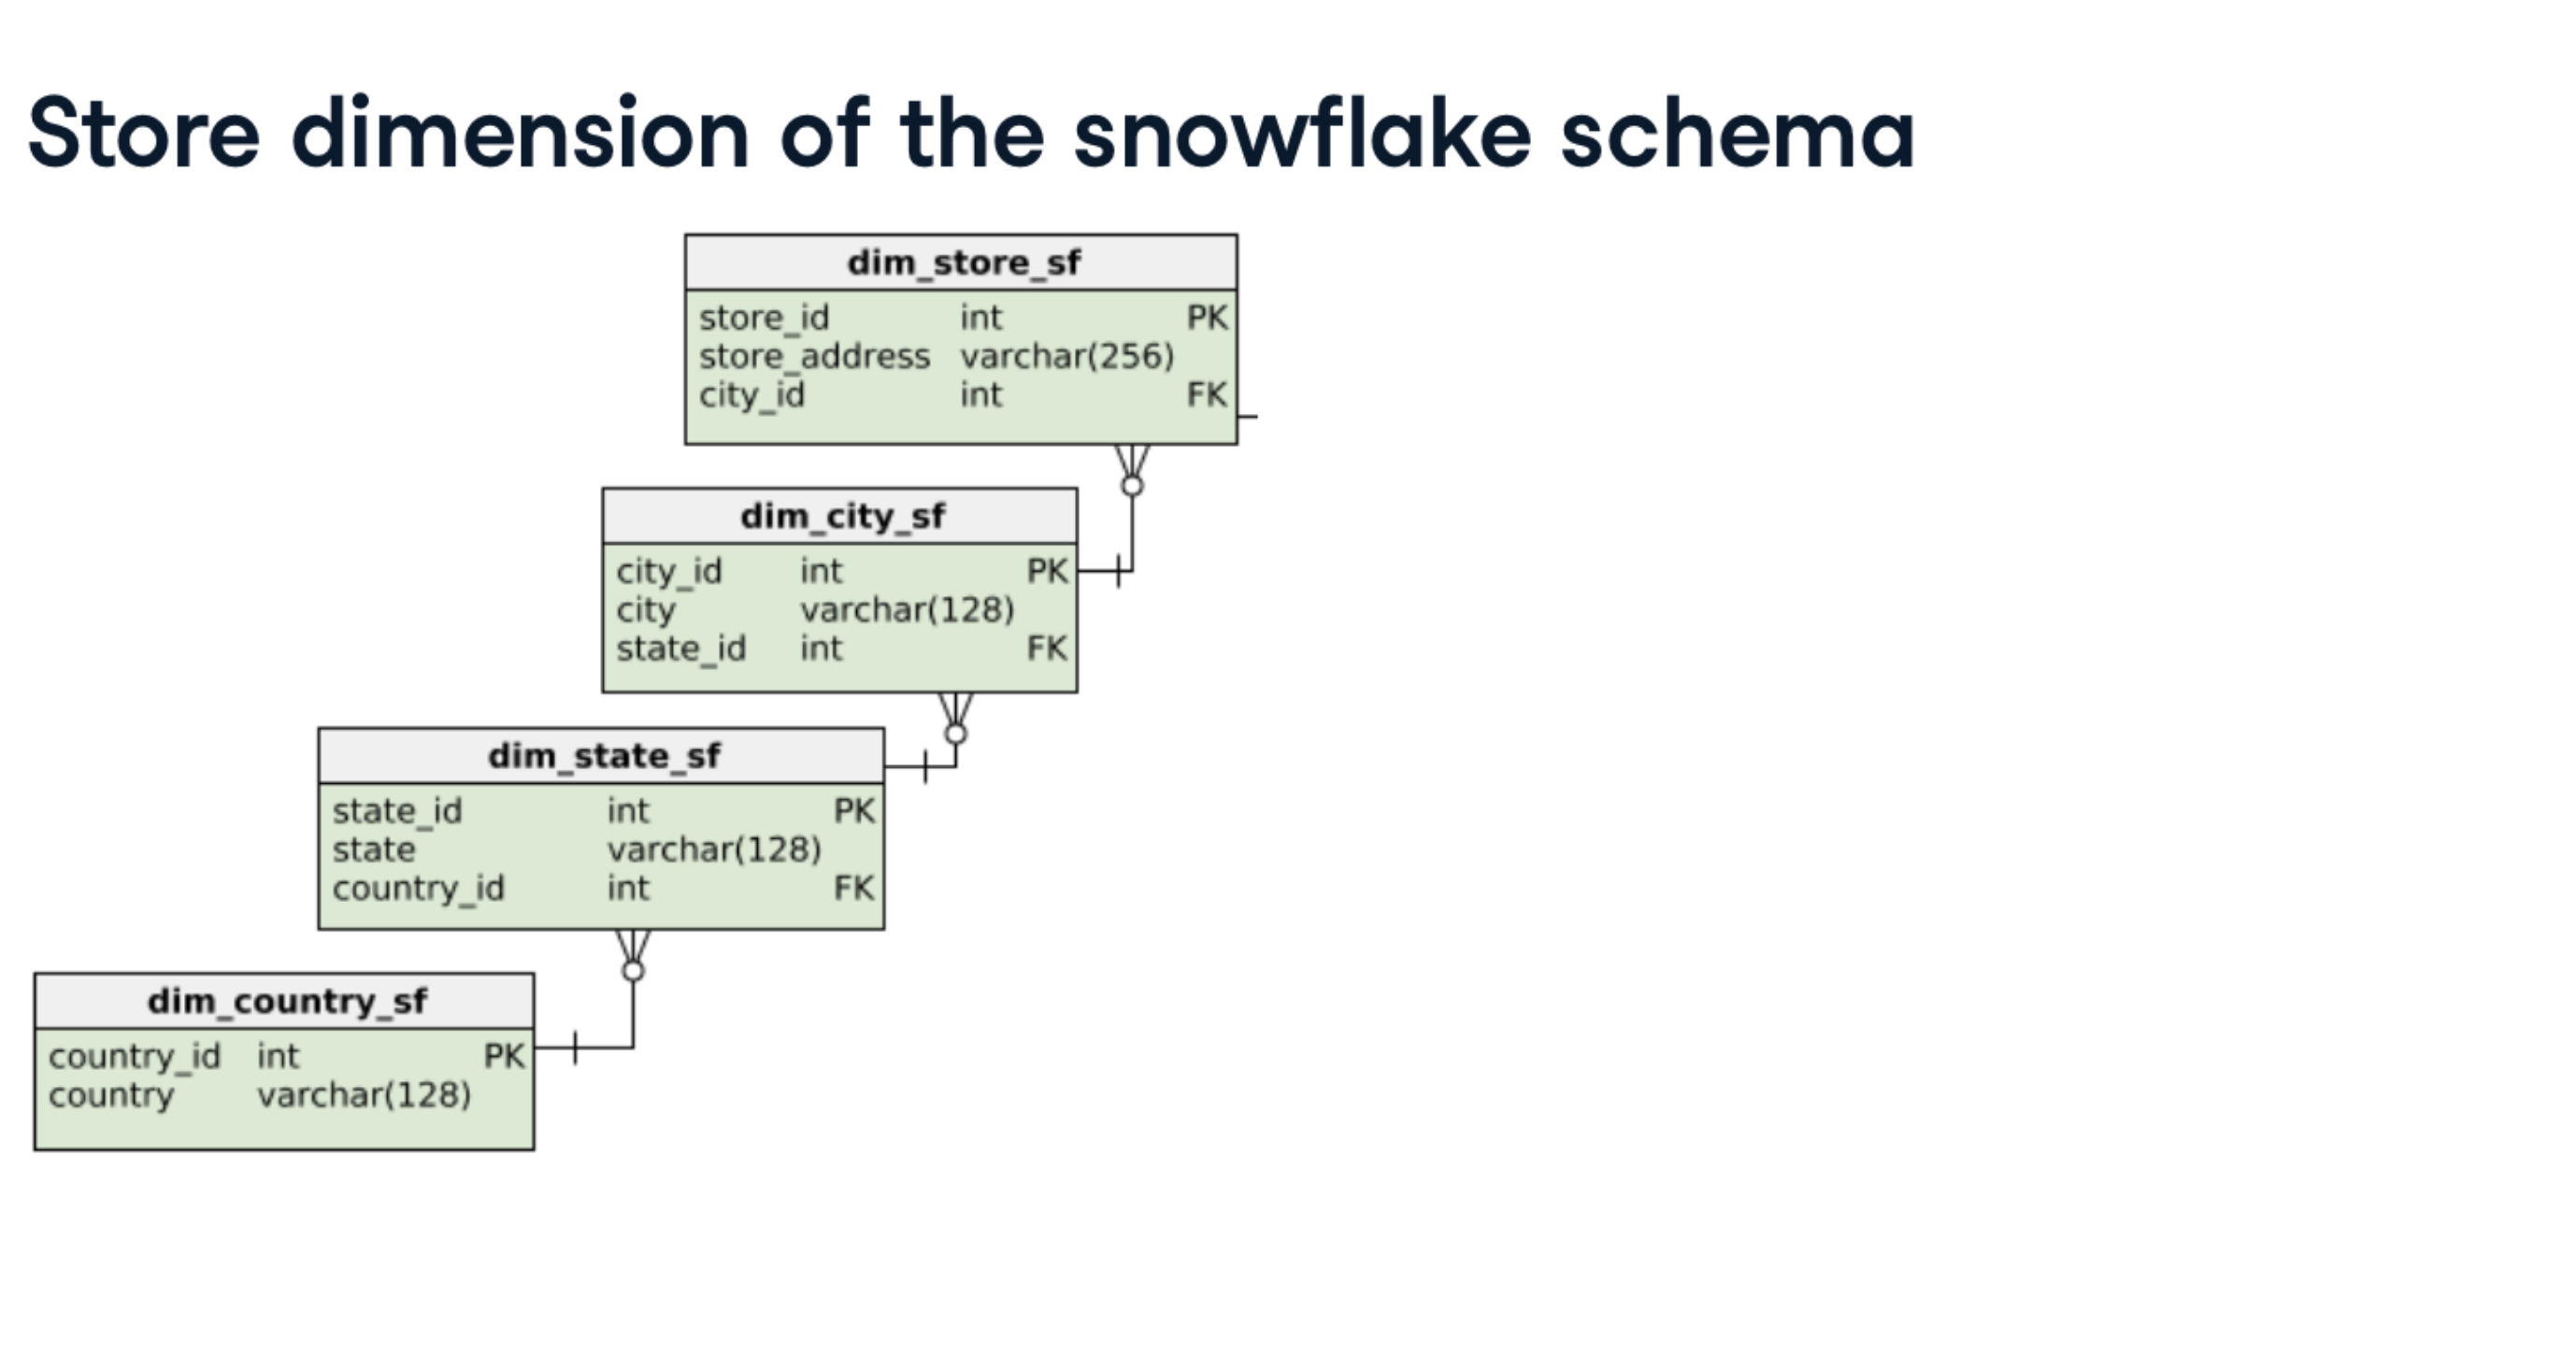
\includegraphics[width=1.0\textwidth]{figures/StoreDimensionExtended.png}
\end{figure}

\begin{figure}[H]
    \centering
    \caption{Comparison of Book And Store Dimension}
    \label{fig:BookAndStoreDimensionComparison}
    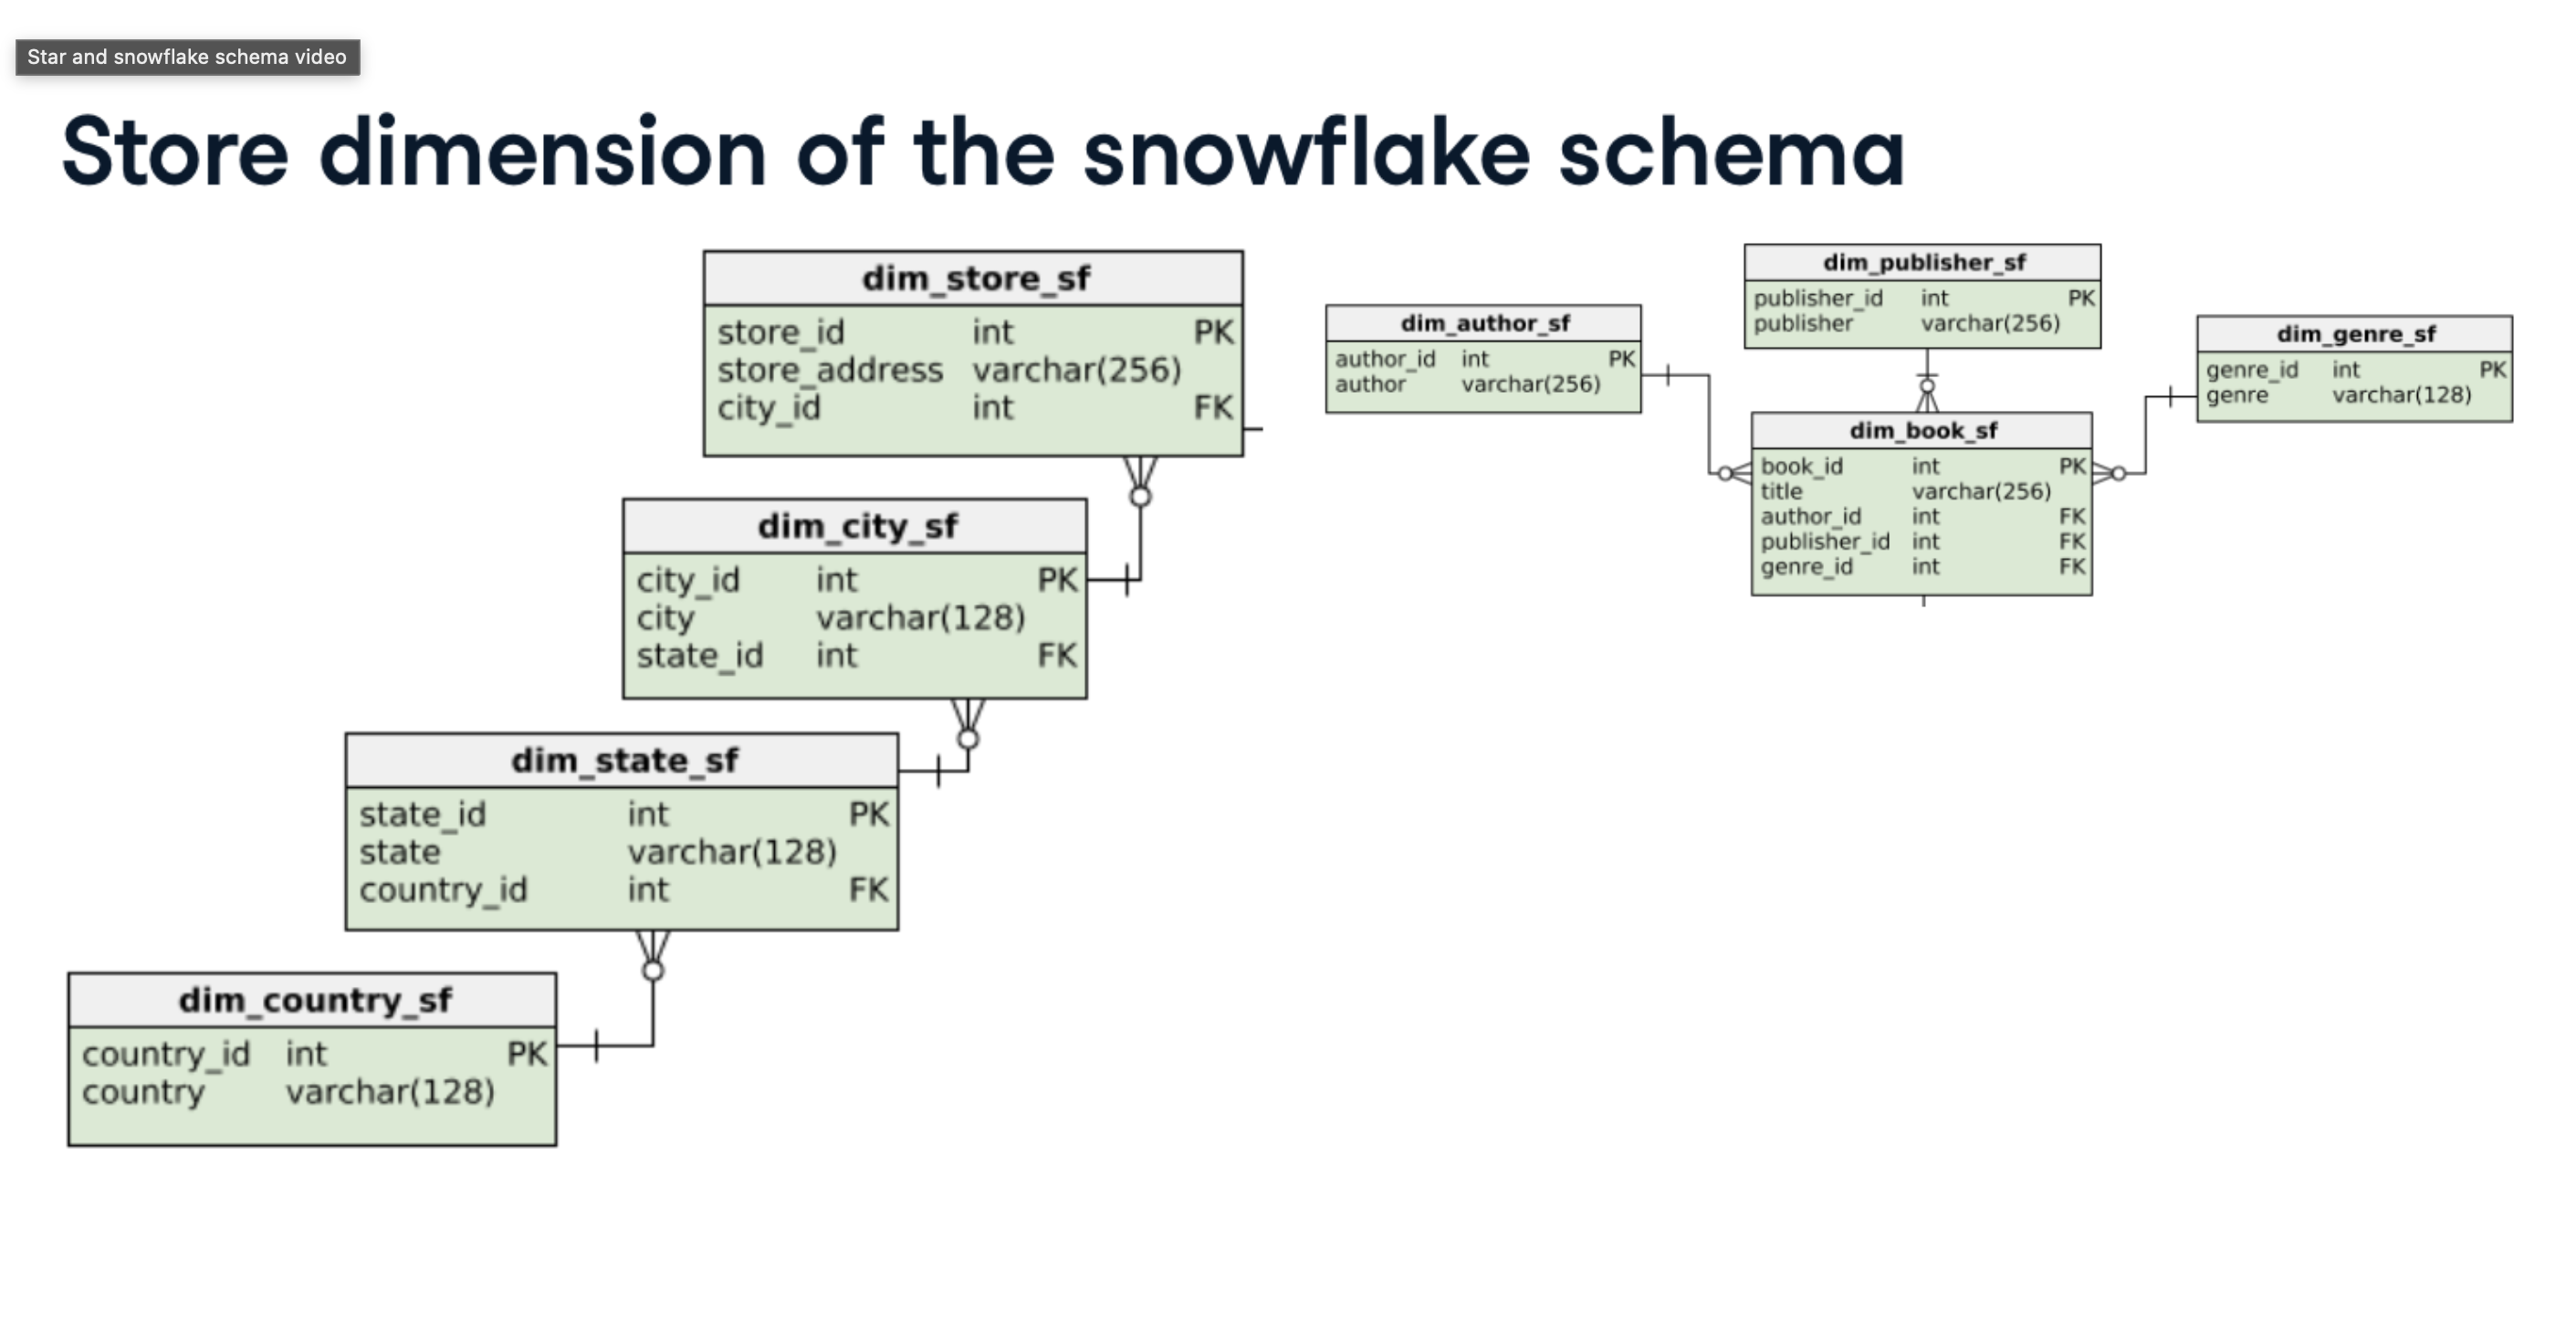
\includegraphics[width=1.0\textwidth]{figures/BookAndStoreDimensionComparison.png}
\end{figure}
Notice how store dimension in \ref{fig:BookAndStoreDimensionComparison} extends iteself, this is because city is part of state and state is part of country.


\begin{figure}[H]
    \centering
    \caption{Time Dimension and its Extension}
    \label{fig:TimeDimensionWithExtension}
    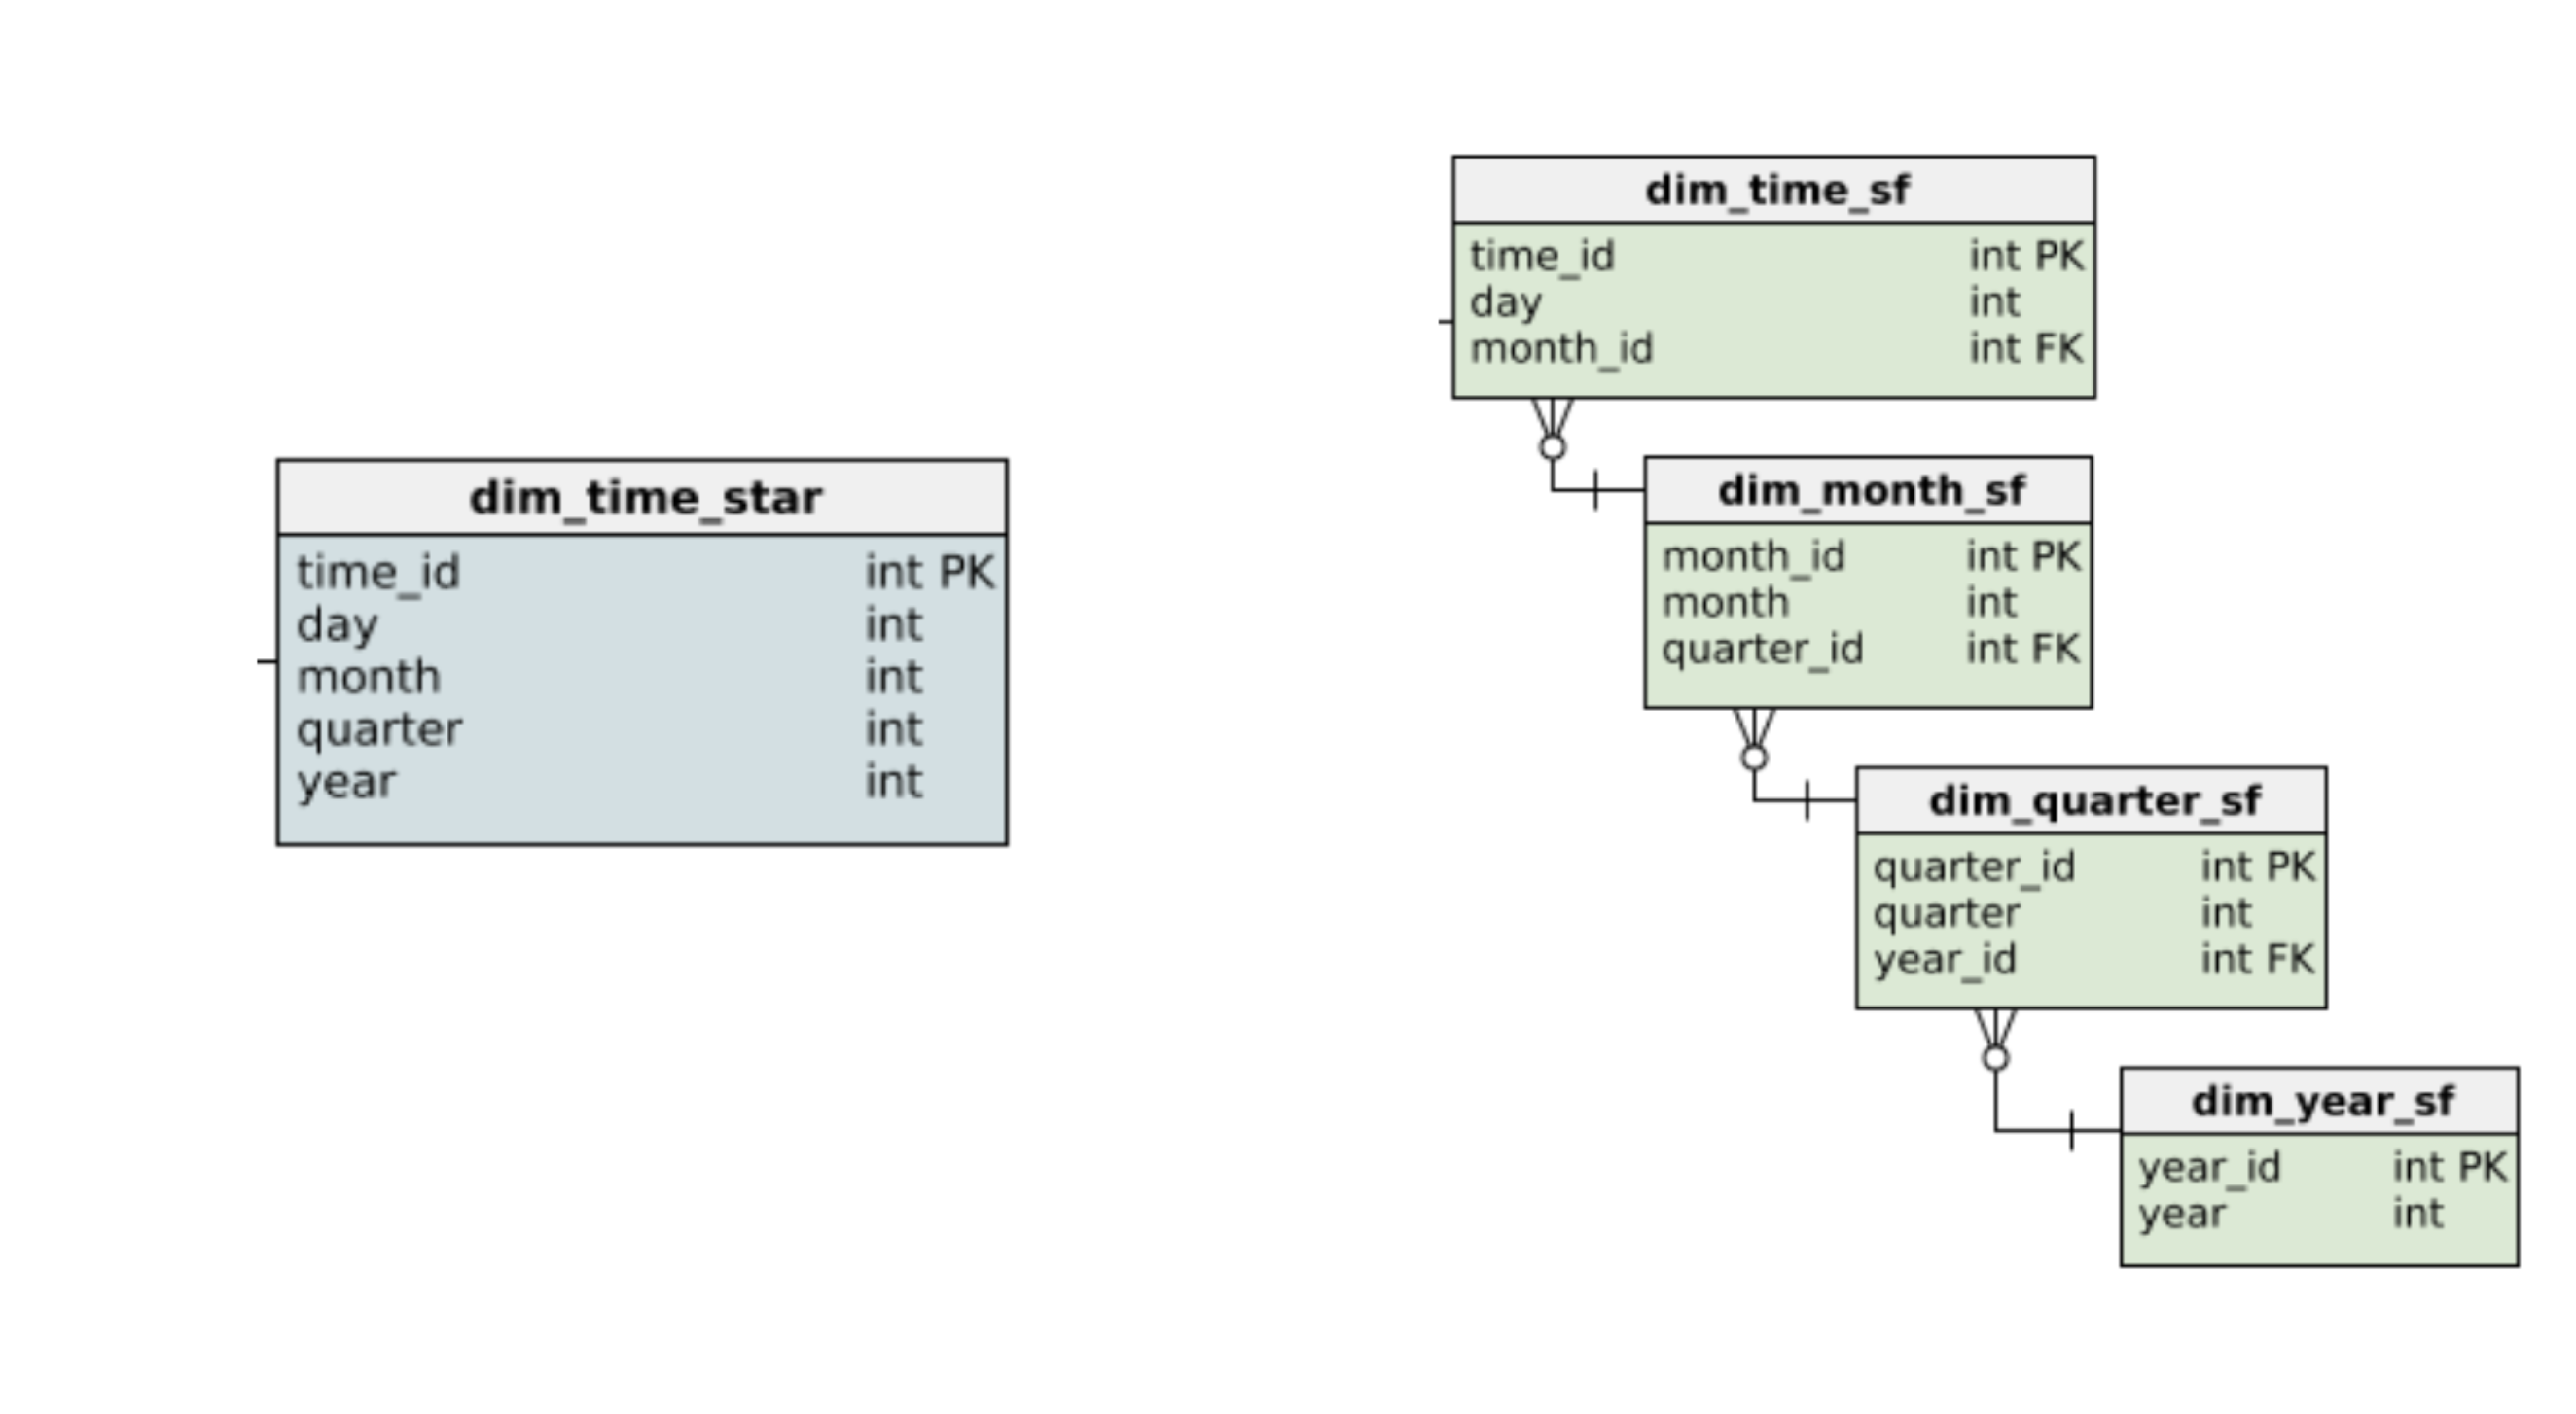
\includegraphics[width=1.0\textwidth]{figures/TimeDimensionWithExtension.png}
\end{figure}

\begin{figure}[H]
    \centering
    \caption{Final Snowflake Schema}
    \label{fig:FinalSnowFlakeSchema}
    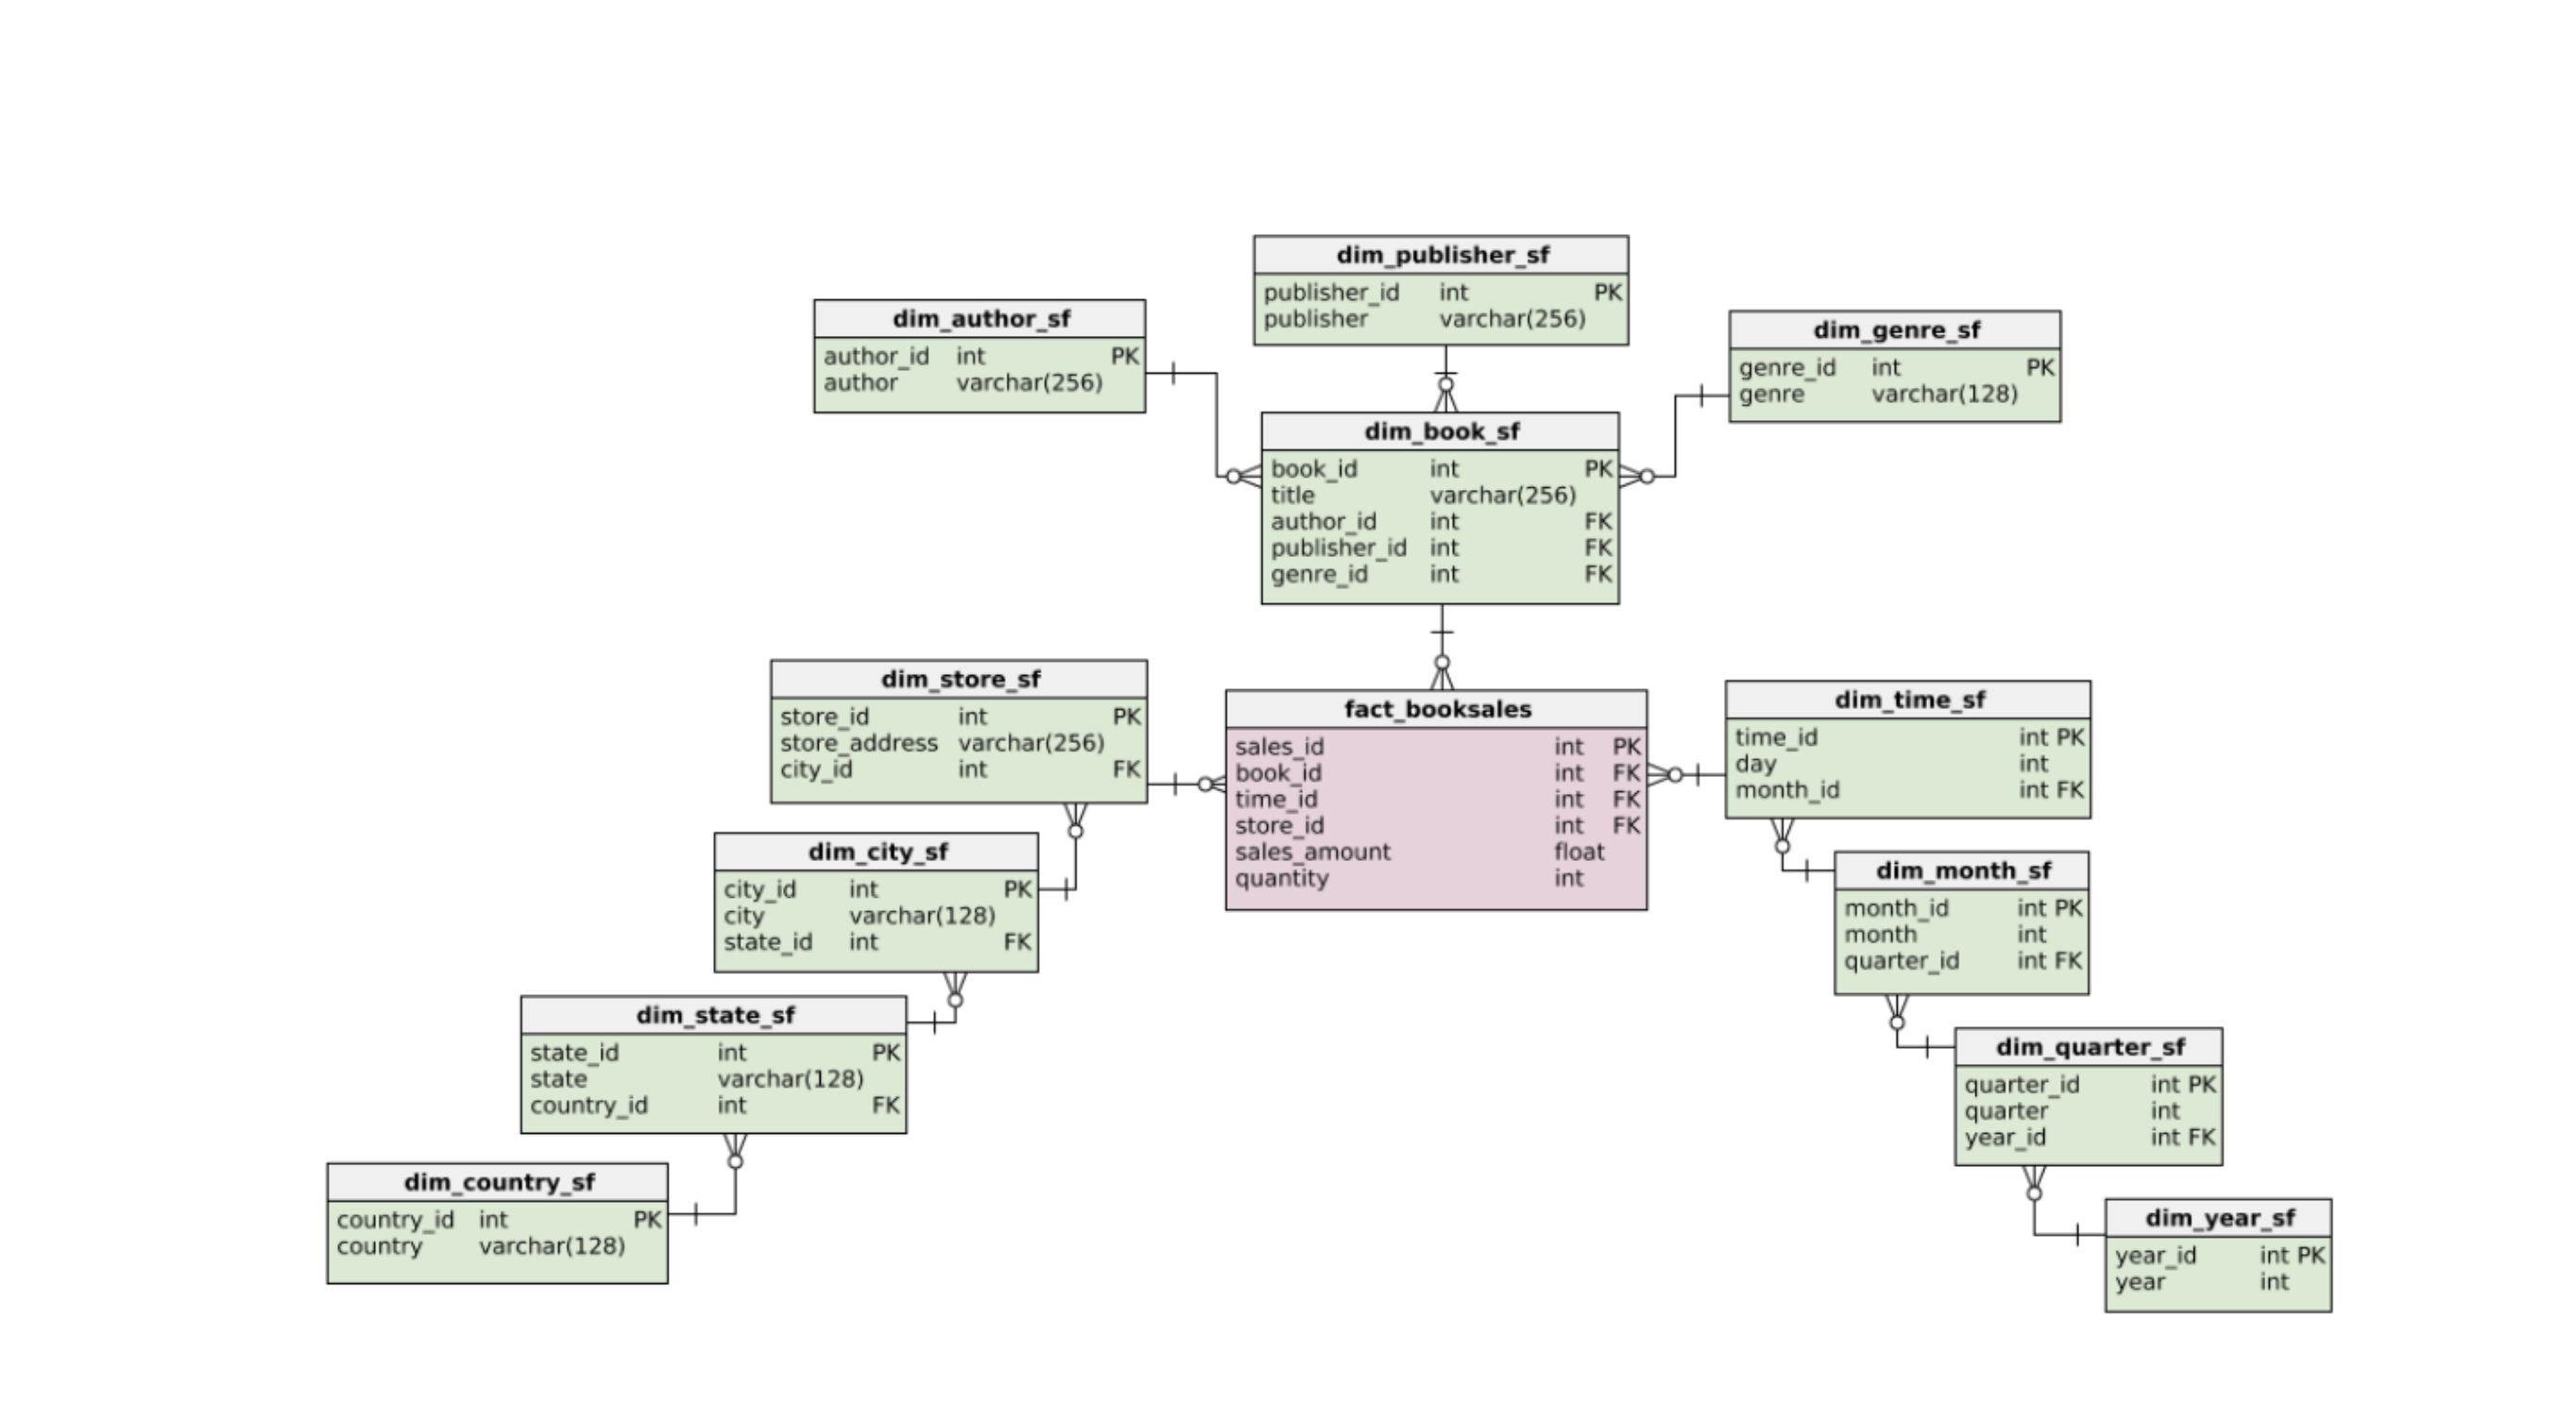
\includegraphics[width=1.0\textwidth]{figures/FinalSnowFlakeSchema.png}
\end{figure}
Putting together all Normalized dimension in \ref{fig:FinalSnowFlakeSchema} we get a SnowflakeSchema from Star Schema.

\subsection{Normalized and denormalized databases}
\begin{figure}[H]
    \centering
    \caption{Normalized Snowflake schema vs Denormalized Star Schema}
    \label{fig:NormCompare}
    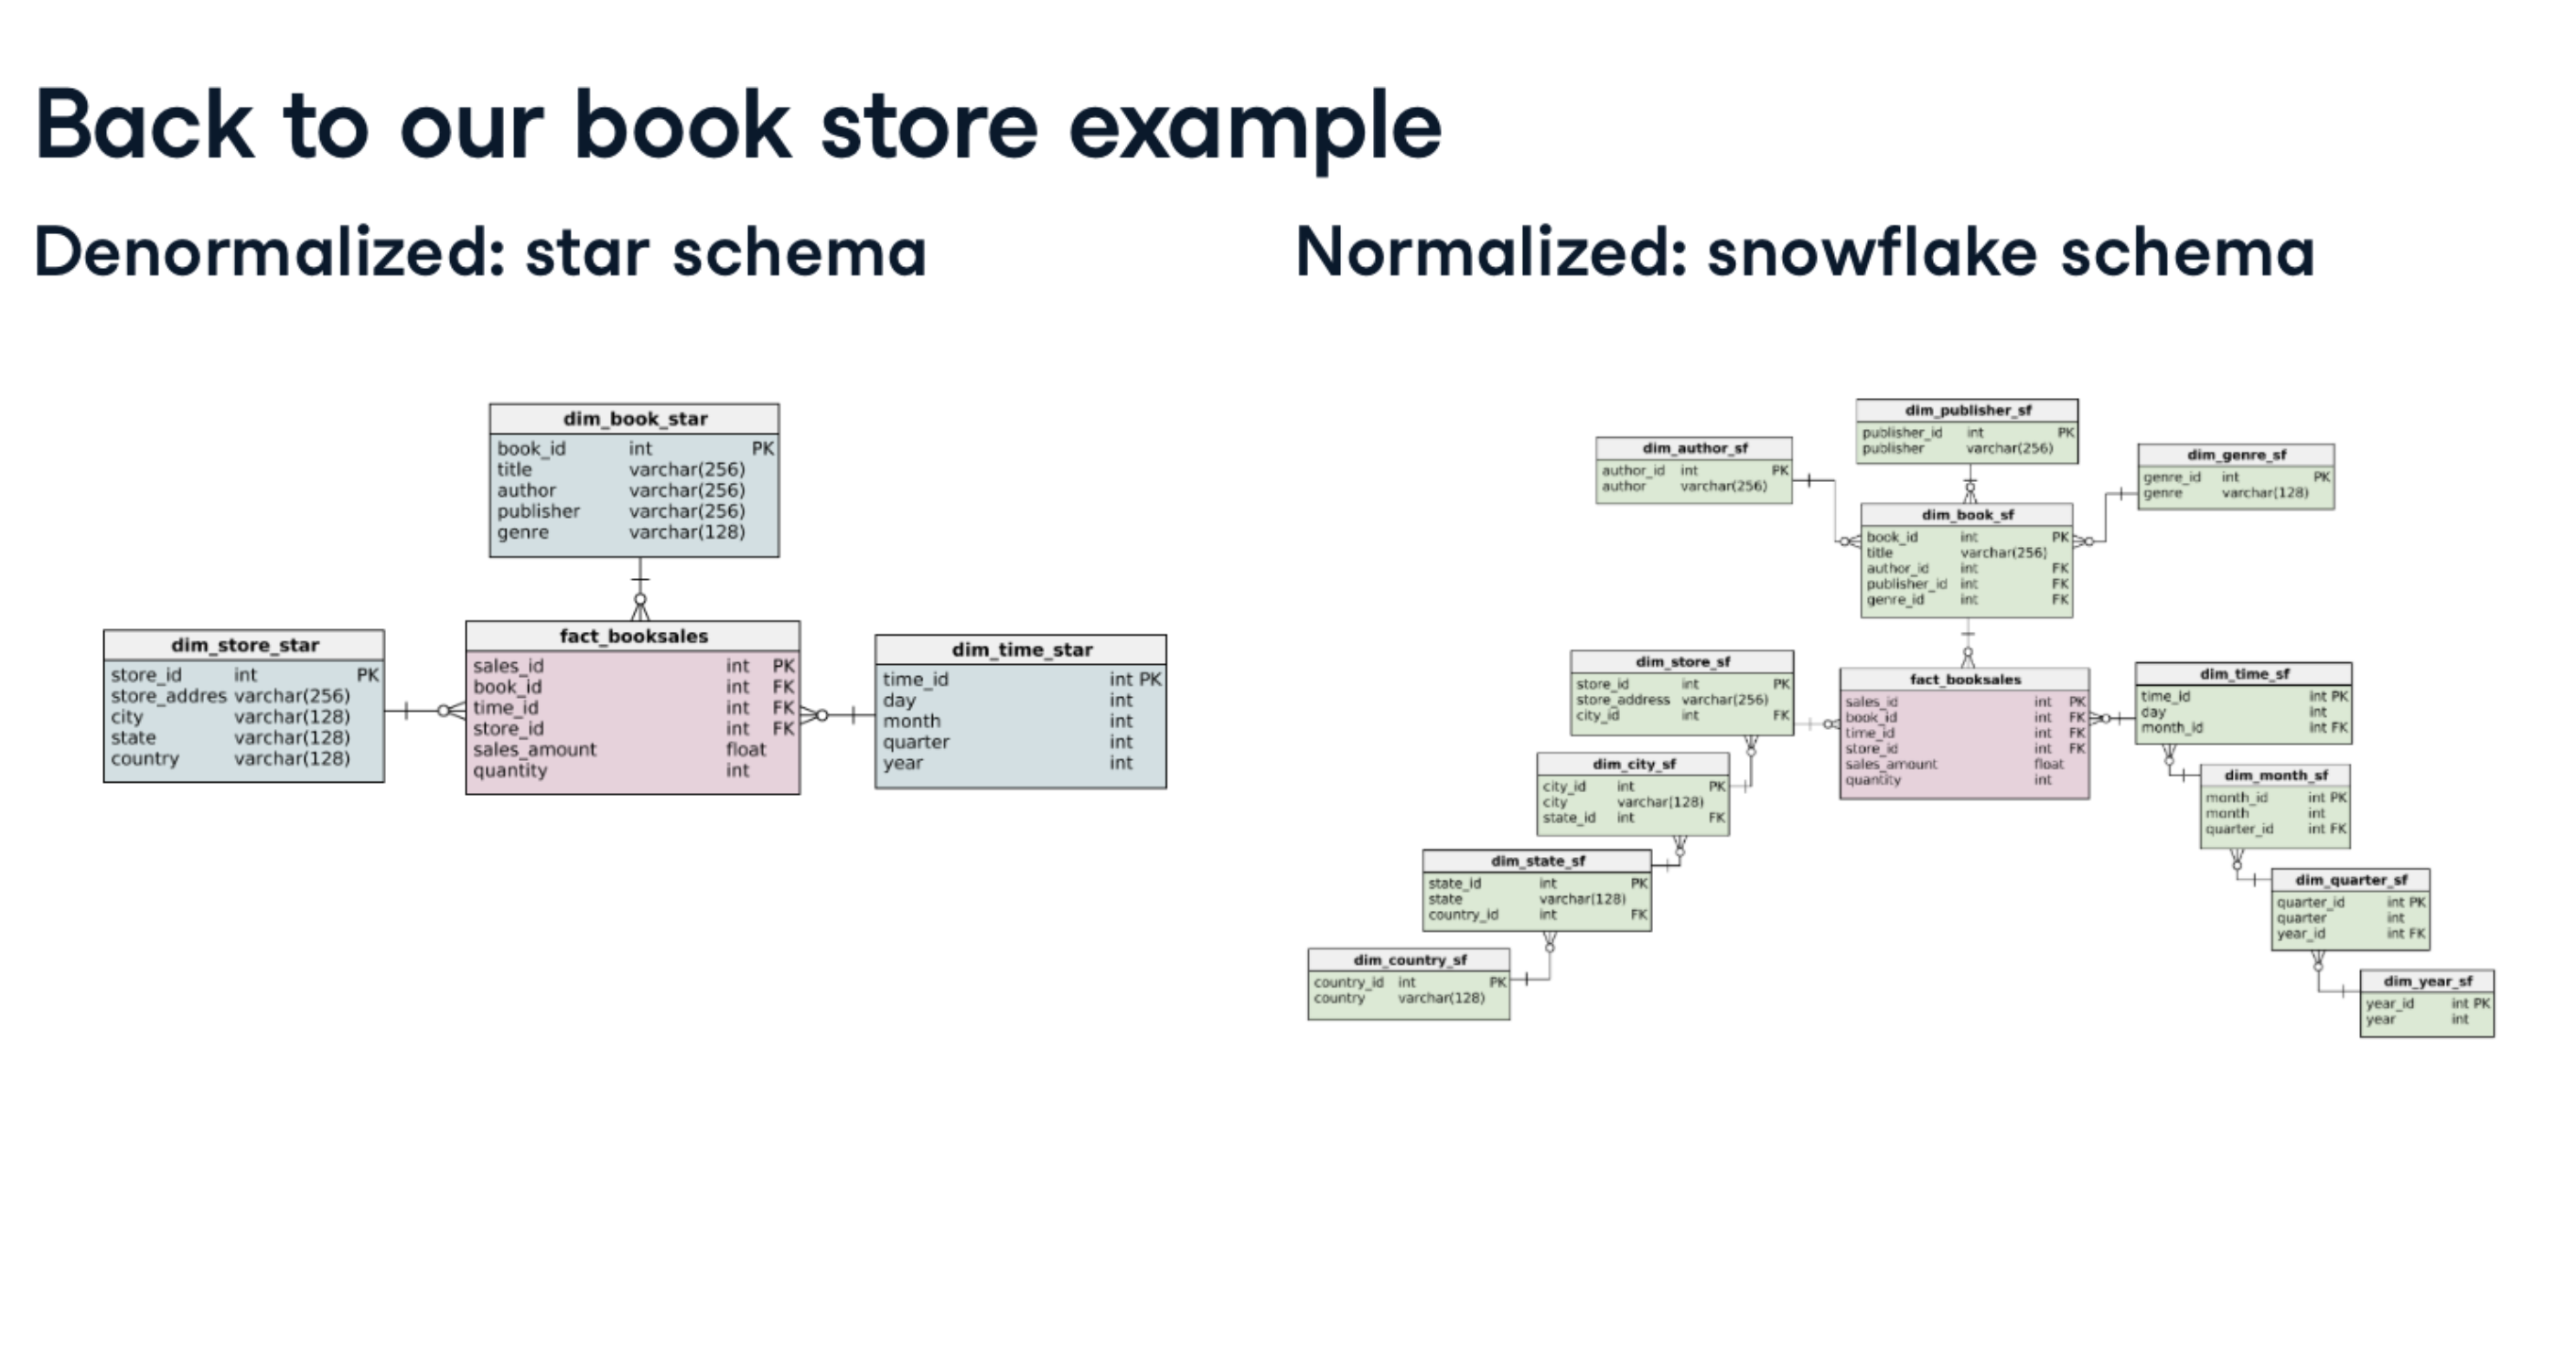
\includegraphics[width=1.0\textwidth]{figures/NormCompare.png}
\end{figure}

\subsubsection{Denormalized Query}
\textbf{Goal:} get quantity of all Octavia E.Butler books sold in Vancouver in Q4 of 2018

\inputminted[
    firstline=1,
    lastline=10
]{SQL}{SQL/DatabaseDesign.sql}

It compose of only 3 joins only which makes it simpler.

\subsubsection{Normalized Query}
\inputminted[
    firstline=12,
    lastline=32
]{SQL}{SQL/DatabaseDesign.sql}
Whereas Normalized Query consist of total 8 joins for the same purpose as it consist of more tables.

\textbf{\emph{So, why would we want to normalize a databases?}} \\
Normalization saves space

\begin{figure}[H]
    \centering
    \caption{Denormalized Table with data redundency}
    \label{fig:Denormalized}
    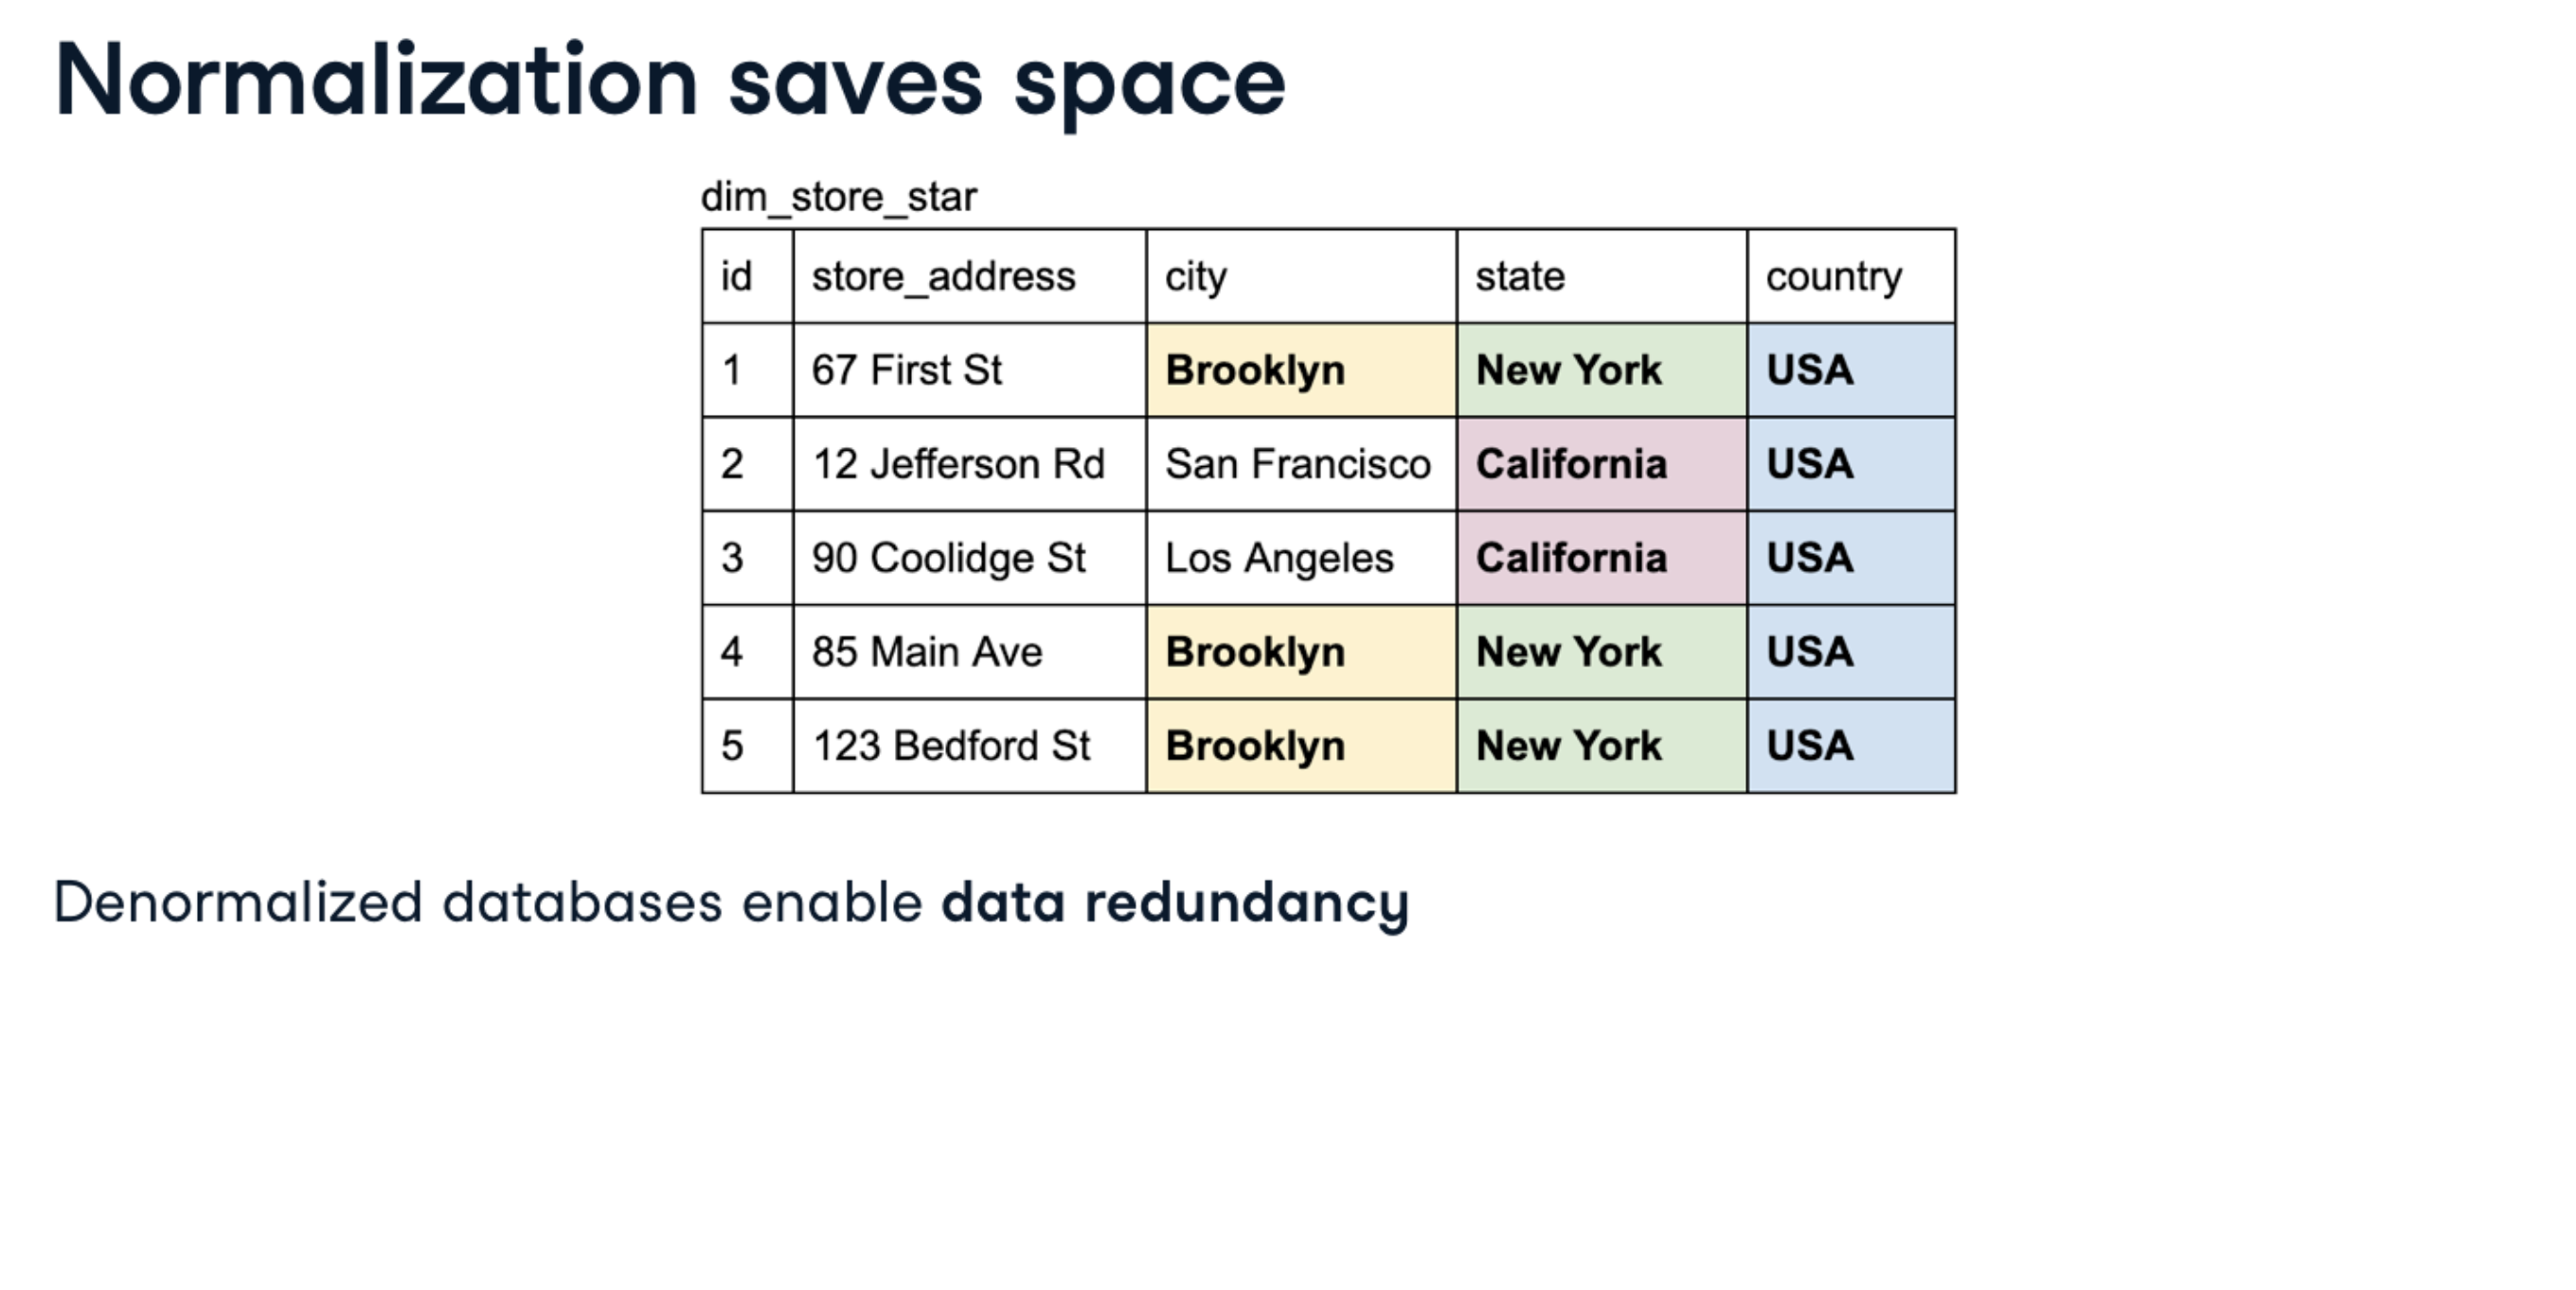
\includegraphics[width=1.0\textwidth]{figures/Denormalized.png}
\end{figure}

\begin{figure}[H]
    \centering
    \caption{Normalized Table}
    \label{fig:Normalized}
    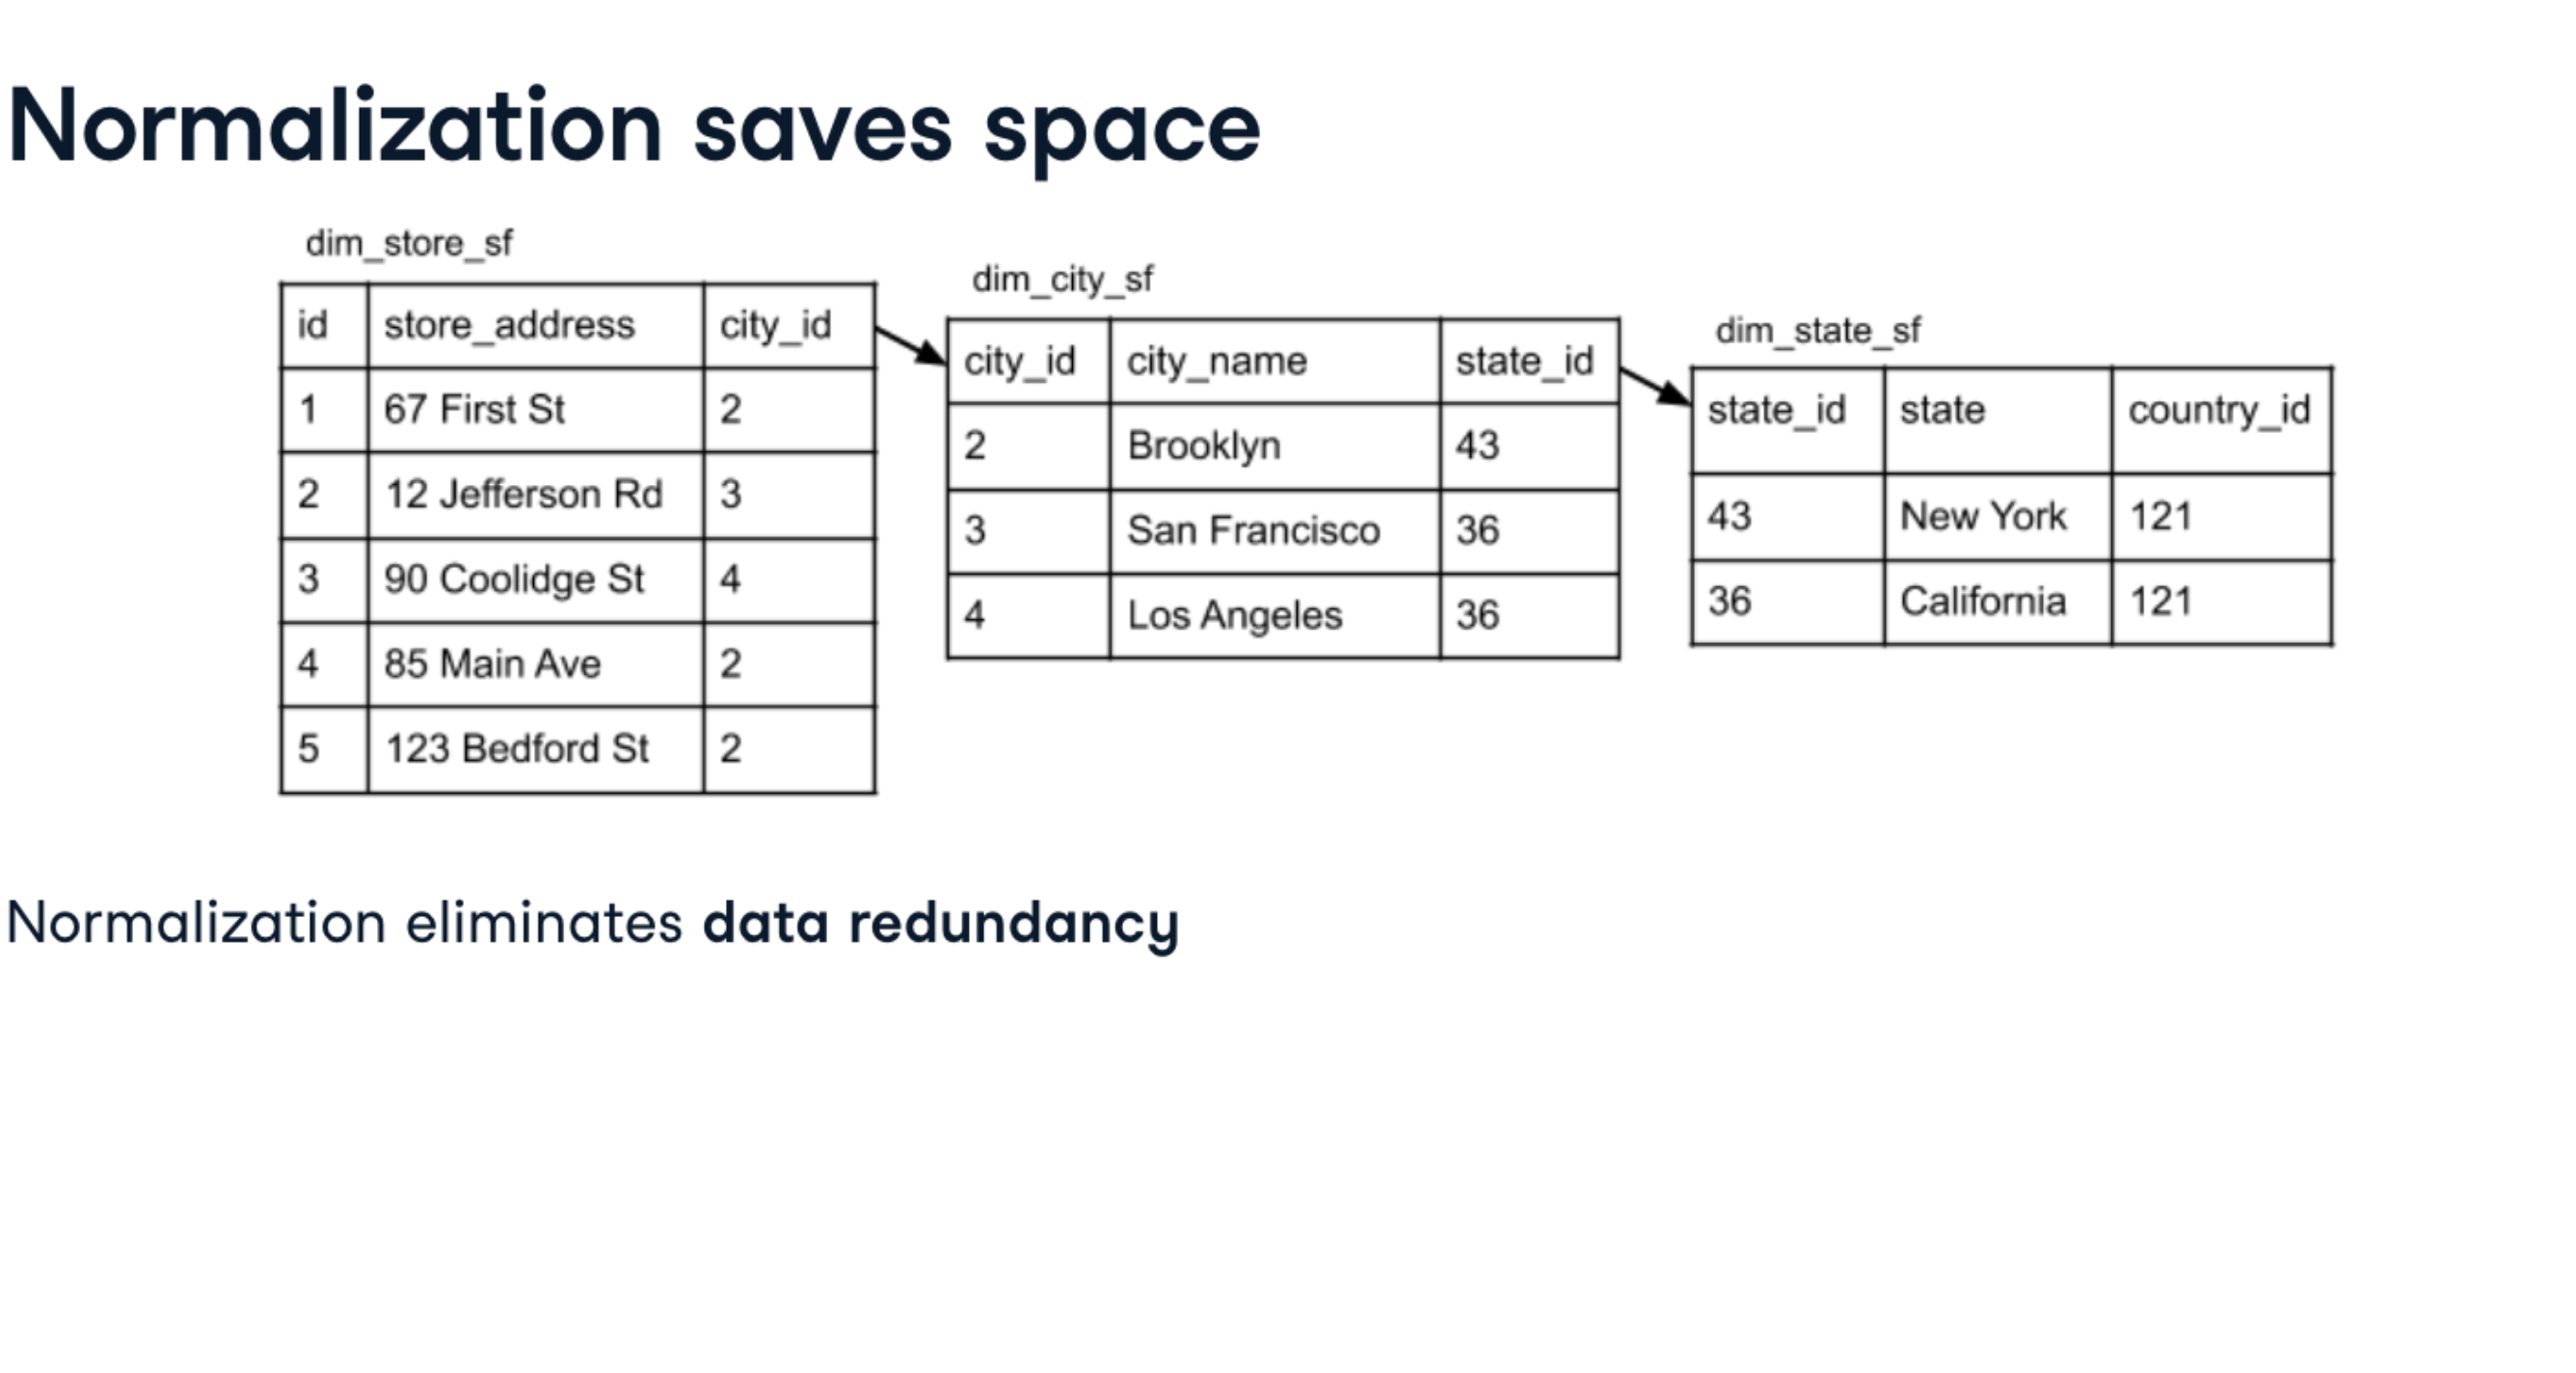
\includegraphics[width=1.0\textwidth]{figures/Normalized.png}
\end{figure}

\subsubsection{Normalization ensures better data integrity}
\begin{enumerate}
    \item \textbf{Enforces data consistency} \\
    Must respect naming conventions because of referential integrity, e.g., 'California', not 'CA' or 'california'
    \item \textbf{Safer updating, removing and inserting} \\
    Less data redundency = less records to alter
    \item \textbf{Easier to redesign by extending} \\
    Smaller tables are easier to extends than larger tables
\end{enumerate}

\subsubsection{Database normalization}
\textbf{Advantages}
\begin{itemize}
    \item Normalization eliminates data redundency: save on storage
    \item Better data integrity: accurate and consistent data
\end{itemize}

\textbf{Disadvantages}
\begin{itemize}
    \item Complex queries require more CPU
\end{itemize}

\subsubsection{OLTP}
e.g., Operational Databases \\
\textbf{Typically highly Normalized}
\begin{itemize}
    \item Write-intensive
    \item Prioritize quicker and safer insertion of data
\end{itemize}

\subsubsection{OLAP}
e.g., Data warehouses \\
\textbf{Typically less Normalized}
\begin{itemize}
    \item Read-intensive
    \item Prioritize quicker queries for analytics
\end{itemize}

\subsection{Normal forms}
\subsubsection{Normalization}
Identify repeating groups of data and create new tables for them. \\
A more formal definition: \\
The goals of normalizationo are to:
\begin{itemize}
    \item Be able to characterize the level of redundency in a relational Schemas
    \item Provide mechanism for transforming schemas in order to remove redundency
\end{itemize}
\emph{Note: From Database Design, 2nd Edition by Adriene Watt}

\subsubsection{Normal forms (NF)}
Ordered from least to most nromalized:
\begin{itemize}
    \item First normal form (1NF)
    \item Second normal form (2NF)
    \item Third normal form (3NF)
    \item Elementary key normal form (EKNF)
    \item Boyce-Codd normal form (BCNF)
    \item Fourth normal form (4NF)
    \item Essential tuple normal form (ETNF)
    \item Fifth normal form (5NF)
    \item Domain-key Normal Form (DKNF)
    \item Sixth normal form (6NF)
\end{itemize}
\emph{Note: from wikipedia Database\_normalization}

\subsubsection{1NF rules}
\begin{itemize}
    \item Each record must be unique-no duplicate rows
    \item Each cell must hold one value
\end{itemize}

Initial data for 1NF
\begin{table}[H]
    \caption{Initial data for 1NF}
    \label{tab:InitialData41NF}
    \begin{tabular}{lll}
        \textbf{Student\_id} & \textbf{Student\_Email} & \textbf{Courses\_Completed} \\
        235 & jim@gmail.com & Introduction to Python, Intermediate Python \\
        455 & kelly@yahoo.com & Cleaning Data in R \\
        767 & amy@hotmail.com & Machine Learning Toolbox, Deep Learning in Python
    \end{tabular}
\end{table}

In 1NF form
\begin{table}[H]
    \begin{tabular}{ll}
        \textbf{Student\_id} & \textbf{Student\_Email} \\
        235 & jim@gmail.com \\
        455 & kelly@yahoo.com \\
        767 & amy@hotmail.com
    \end{tabular}
\end{table}

\begin{table}[H]
    \begin{tabular}{ll}
        \textbf{Student\_id} & \textbf{Completed} \\
        235 & Introduction to Python \\
        235 & Intermediate Python \\
        455 & Cleaning Data in R \\
        767 & Machine Learning Toolbox \\
        767 & Deep Learning in Python
    \end{tabular}
\end{table}

\subsubsection{2NF}
\begin{itemize}
    \item Must satisfy 1NF AND
    \begin{itemize}
        \item If primary key is one column
        \begin{itemize}
            \item then automatically satisfies 2NF
        \end{itemize}
        \item If there is a composite primary key
        \begin{itemize}
            \item then each non-key column must be dependent on all the keys
        \end{itemize}
    \end{itemize}
\end{itemize}

Initial data for 2NF
\begin{table}[H]
    \caption{Initial data for 2NF}
    \label{tab:InitialData42NF}
    \begin{tabular}{lllll}
        \textbf{Student\_id (PK)} & \textbf{Course\_id (PK)} & \textbf{Instructor\_id} & \textbf{Instructor} & \textbf{Progress} \\
        235 & 2001 & 560 & Nick Carchedi & .55 \\
        455 & 2345 & 658 & Ginger Grand & .10\\
        767 & 6584 & 999 & Chester Ismay & 1.00
    \end{tabular}
\end{table}

In 2NF form
\begin{table}[H]
    \begin{tabular}{lll}
        \textbf{Student\_id (PK)} & \textbf{Course\_id (PK)} & \textbf{Percent\_Completed} \\
        235 & 2001 & .55 \\
        455 & 2345 & .10 \\
        767 & 6584 & 1.00 \\
    \end{tabular}
\end{table}

\begin{table}[H]
    \begin{tabular}{lll}
        \textbf{Course\_id (PK)} & \textbf{Instructor\_id} & \textbf{Instructor} \\
        2001 & 560 & Nick Carchedi \\
        2345 & 658 & Ginger Grand \\
        6584 & 999 & Chester Ismay
    \end{tabular}
\end{table}

\subsubsection{3NF}
\begin{itemize}
    \item Satisfies 2NF
    \item No \textbf{transitive dependencies}: non-key columns can't depend on other non-key columns
\end{itemize}

Initial Data for 3NF
\begin{table}[H]
    \caption{Initial data for 3NF}
    \label{tab:InitailData43NF}
    \begin{tabular}{llll}
        \textbf{Course\_id (PK)} & \textbf{Instructor\_id} & \textbf{Instructor} & \textbf{Tech} \\
        2001 & 560 & Nick Carchedi & Python \\
        2345 & 658 & Ginger Grand & SQL \\
        6584 & 999 & Chester Ismay & R
    \end{tabular}
\end{table}

In 3NF
\begin{table}[H]
    \begin{tabular}{lll}
        \textbf{Course\_id (PK)} & \textbf{Instructor} & \textbf{Tech} \\
        2001 & Nick Carchedi & Python \\
        2345 & Ginger Grand & SQL \\
        6584 & Chester Ismay & R
    \end{tabular}
\end{table}

\begin{table}[H]
    \begin{tabular}{ll}
        \textbf{Instructor\_id} & \textbf{Instructor} \\
        560 & Nick Carchedi \\
        658 & Ginger Grand \\
        999 & Chester Ismay
    \end{tabular}
\end{table}

\subsubsection{Data anomolies}
\emph{What is risked if we don't normalize enough?}
\begin{enumerate}
    \item \textbf{Update anomaly} \\
    \textbf{Data inconsistency caused by data redundancy when updating}
    \begin{table}[H]
        \caption{Student records}
        \label{tab:StudentRecords}
        \begin{tabular}{llll}
        \textbf{Student\_ID} & \textbf{Student\_Email} & \textbf{Enrolled\_in} & \textbf{Taught\_by} \\
        230 & lisa@gmail.com & Cleaning Data in R & Maggie Matsui \\
        367 & bob@hotmail.com & Data Visualization in R & Ronald Pearson \\
        520 & ken@yahoo.com & Introduction to Python & Hugo Bowne-Anderson \\
        520 & ken@yahoo.com & Arima Models in R & David Stoffer \\
        \end{tabular}
    \end{table}
    To update student \textbf{520}'s email:
    \begin{itemize}
        \item Need to update mroe than one records, otherwise, there will be inconsistency
        \item User updating needs to know about redundancy
    \end{itemize}
    \item \textbf{Insertion anomaly} \\
    \textbf{Unable to add a record due to missing attributes} \\
    In table \ref{tab:StudentRecords}, Unable to insert a student who has signed up but not enrolled in any courses
    \item \textbf{Deletion anomaly}
    \textbf{Deletion of record(s) causes unintentional loss of data} \\
    In table \ref{tab:StudentRecords}, If we delete Student \textbf{230}, what happens to the data on \textbf{Cleaning Data in R}, we risk deleting course data itself
\end{enumerate}

The more normalized the database, the less prone it will be to data anomalies.

\subsection{Database Views}
\subsubsection{Database Views}
In a database, a \textbf{view} is the result set of a stored query on data, which the 
database users can query just as they would in a persistent database collection Object \emph{(Wikipedia)}.

\textbf{Virtual table that is not part of the physical schema}
\begin{itemize}
    \item Query, not data, is stored in memory
    \item Data is aggregated from data in tables
    \item Can be queried like a regular database table
    \item No need to retype common queries or alter Schemas
\end{itemize}

\subsubsection{Creating a view (syntax)}
\inputminted[
    firstline=34,
    lastline=37,
    highlightlines=34
]{SQL}{SQL/DatabaseDesign.sql}

\subsubsection{Creating a view (Example)}
\begin{figure}[H]
    \centering
    \caption{Create a view scifi genre}
    \label{fig:CreatingView}
    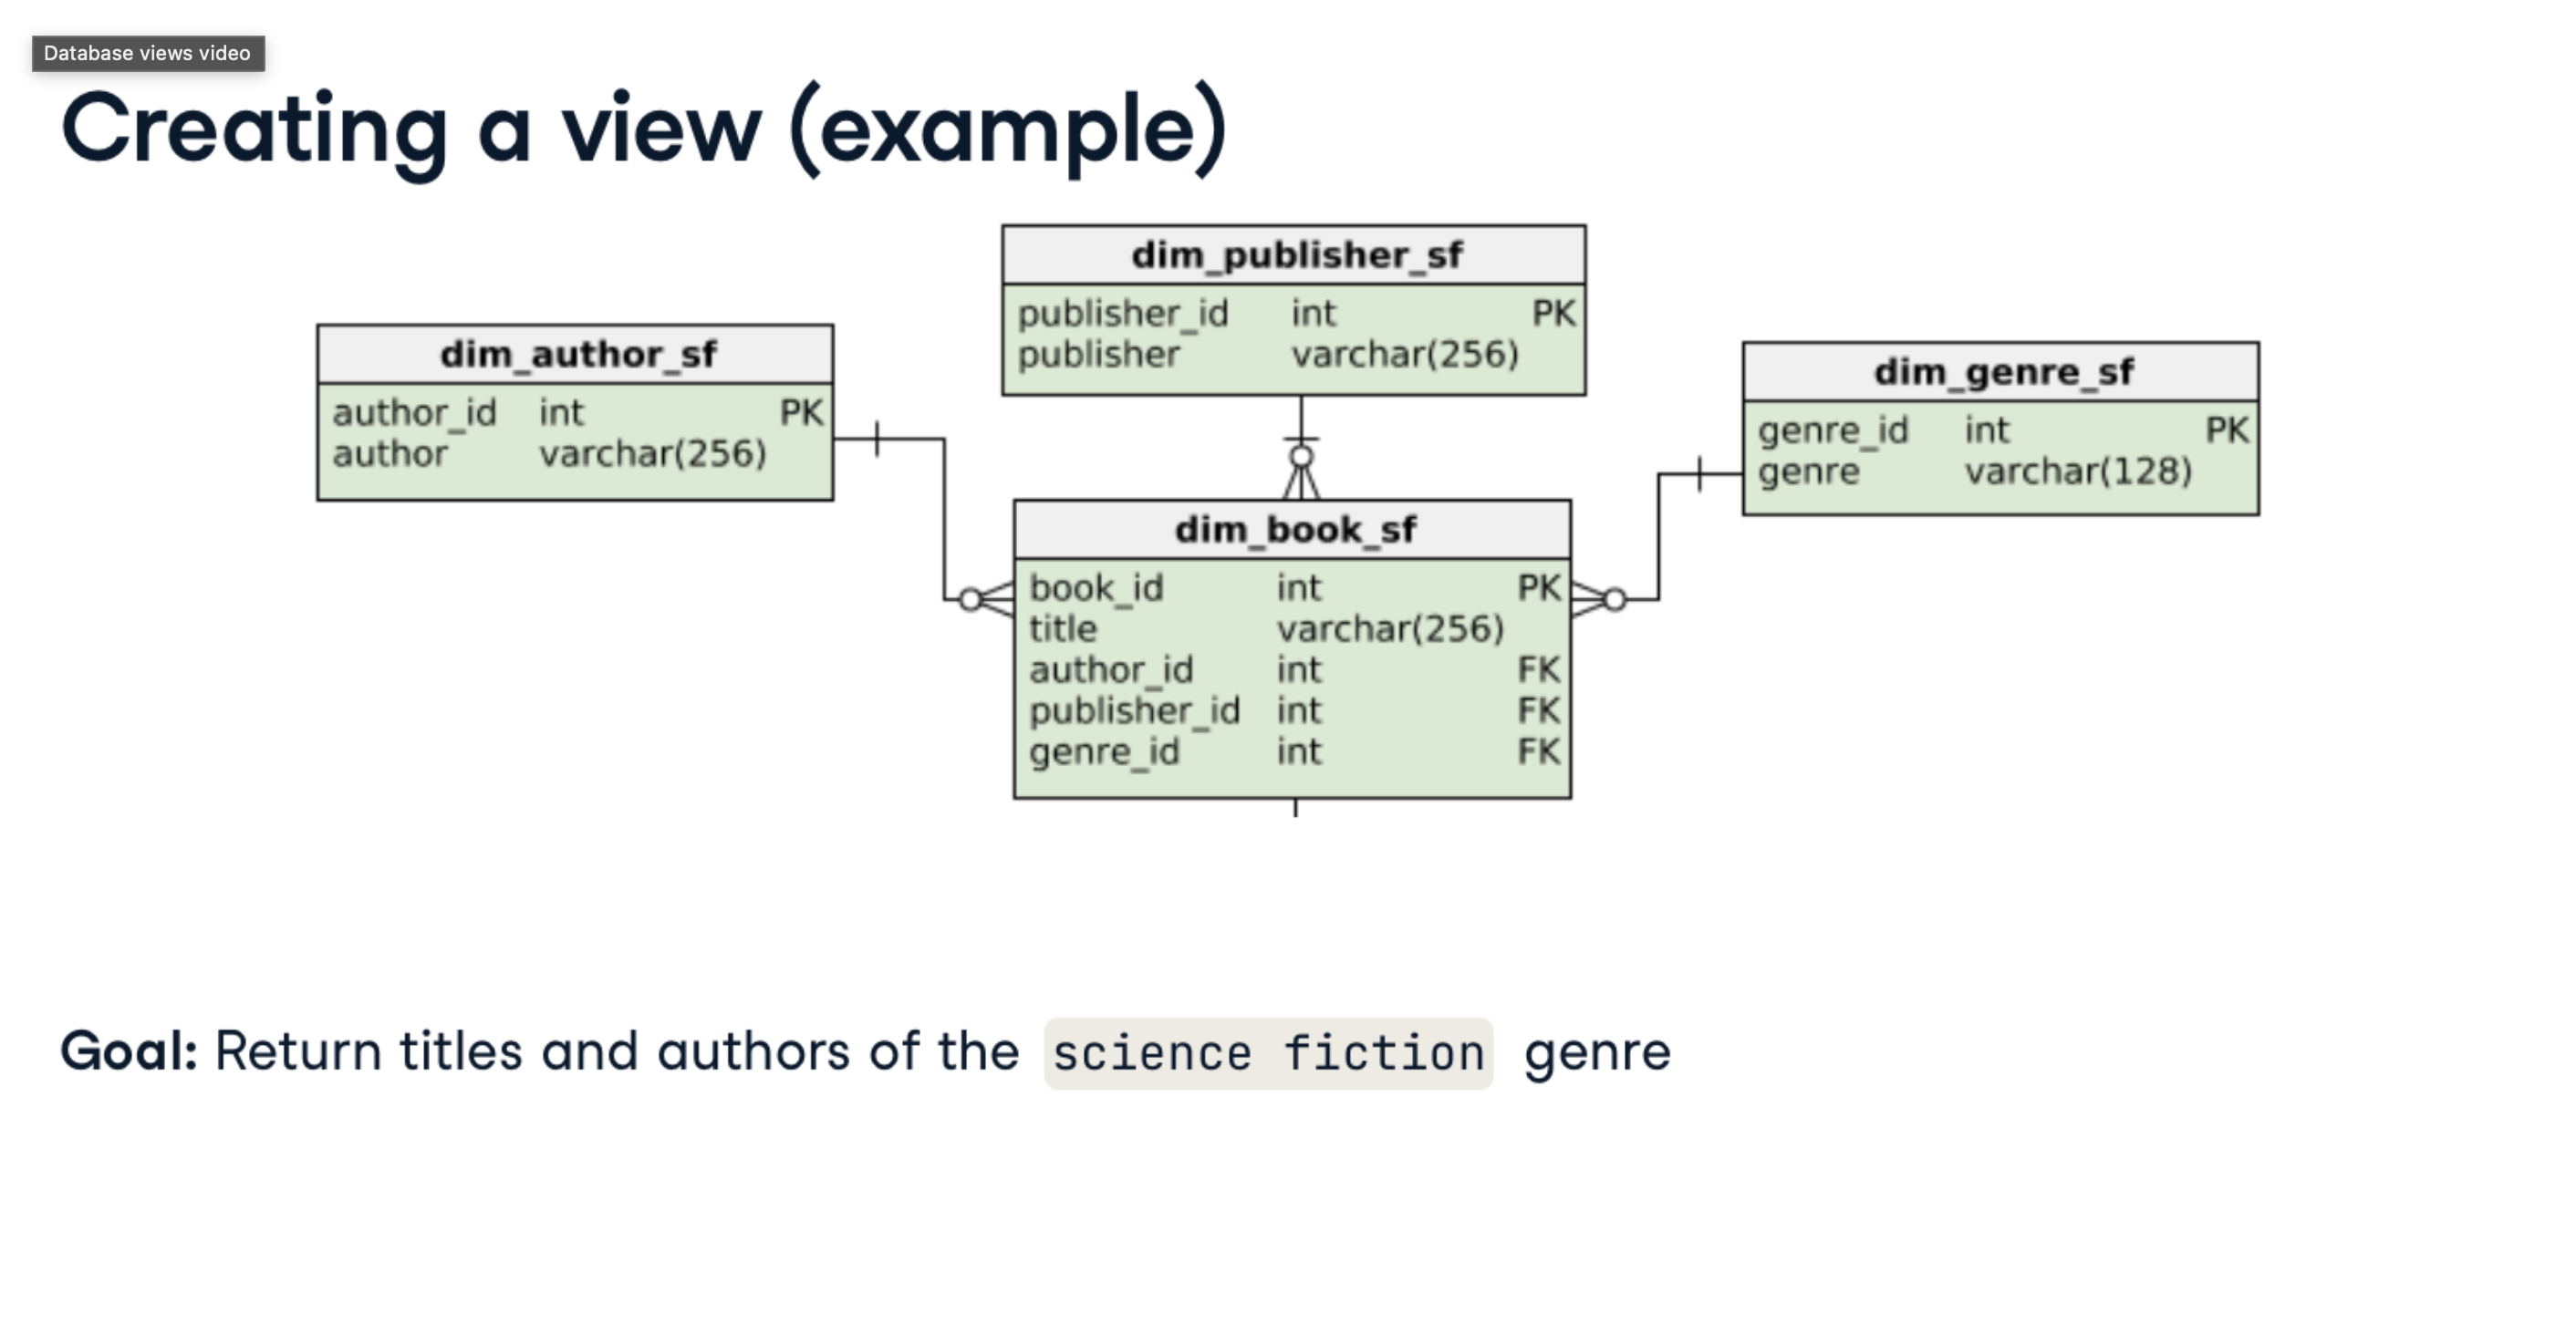
\includegraphics[width=1.0\textwidth]{figures/CreatingView.png}
\end{figure}

\inputminted[
    firstline=39,
    lastline=44,
    highlightlines=39
]{SQL}{SQL/DatabaseDesign.sql}

\subsubsection{Querying a view (Example)}
\inputminted[
    firstline=46,
    lastline=46,
    highlightlines=46
]{SQL}{SQL/DatabaseDesign.sql}

\begin{table}[H]
    \caption{Querying a view}
    \label{tab:QueryView}
    \begin{tabular}{lll}
        \textbf{title} & \textbf{author} & \textbf{genre} \\
        The Naked Sun & Issac Asimov & science fiction \\
        The Robots of Dawn & Issac Asimov & science fiction \\
        The Time Machine & H.G. Wells & science fiction \\
        The Invisible Man & H.G. Wells & science fiction \\
        ... & ... & ...
    \end{tabular}
\end{table}

\textbf{\emph{scifi\_books}} isn\'t an actual table when 
\inputminted[
    firstline=46,
    lastline=46
]{SQL}{SQL/DatabaseDesign.sql}
is run, it runs 
\inputminted[
    firstline=48,
    lastline=53
]{SQL}{SQL/DatabaseDesign.sql}

\subsubsection{Viewing Views}
(in PostgreSQL)

\inputminted[
    firstline=55,
    lastline=55
]{SQL}{SQL/DatabaseDesign.sql}
Above query includes system views, to exclude

\inputminted[
    firstline=57,
    lastline=58
]{SQL}{SQL/DatabaseDesign.sql}
Excludes system views

\subsubsection{Benefits of Views}
\begin{itemize}
    \item Doesn't take up storage
    \item A form of \textbf{access control}
    \begin{itemize}
        \item Hide sensitive columns and restrict what user can see
    \end{itemize}
    \item Masks complexity of queries
    \begin{itemize}
        \item Useful for highly normalized schemas
    \end{itemize}
\end{itemize}

\subsection{Managing views}
\subsubsection{Creating more complex views}
\begin{itemize}
    \item \textbf{Aggregation:} SUM(), AVG(), COUNT(), MIN(), MAX(), GROUP BY, etc
    \item \textbf{Joins:} INNER JOIN, LEFT JOIN, RIGHT JOIN, FULL JOIN
    \item \textbf{Conditionals:} WHERE, HAVING, UNIQUE, NOT NULL, AND, OR, >, <, etc
\end{itemize}
\emph{Note: Be aware of long execution times of views}

\subsubsection{Granting and revoking access to a views}
\hl{GRANT privilege(s)} or \hl{REVOKE privilege(s)}

\hl{ON Object}

\hl{TO role} or \hl{FROM role}

\begin{itemize}
    \item \textbf{Privileges:} \hl{SELECT}, \hl{INSERT}, \hl{UPDATE}, \hl{DELETE}, etc
    \item \textbf{Objects:} table, view, schema, etc
    \item \textbf{Roles:} a database user or a group of databaes users
\end{itemize}

\subsubsection{Granting and revoking example}
\inputminted[
    firstline=60,
    lastline=62
]{SQL}{SQL/DatabaseDesign.sql}

\emph{Note: Here PUBLIC encompasses all users of the database.}

\subsubsection{Updating a view}
\inputminted[
    firstline=64,
    lastline=64
]{SQL}{SQL/DatabaseDesign.sql}

\textbf{Not all views are updatable}
\begin{itemize}
    \item View is made up of one table
    \item Doesn't use a window or aggregate function
\end{itemize}

\subsubsection{Inserting into a view}
\inputminted[
    firstline=66,
    lastline=67
]{SQL}{SQL/DatabaseDesign.sql}

\textbf{Not all views are insertable}
\emph{Takeaway: avoid modifying data through views}

\subsubsection{Dropping a view}
\inputminted[
    firstline=69,
    lastline=69
]{SQL}{SQL/DatabaseDesign.sql}

\begin{itemize}
    \item \hl{RESTRICT} (default): returns an error if there are objects that depend on the view
    \item \hl{CASCADE}: drops view and any object that depends on that view
\end{itemize}

\subsubsection{Redefining a view}
\inputminted[
    firstline=71,
    lastline=71
]{SQL}{SQL/DatabaseDesign.sql}
\begin{itemize}
    \item If a view with \hl{view\_name} exists, it is replaced
    \item \hl{new\_query} must generate the same column names, order and data types as the old query
    \item The column output may be Different
    \item New columns may be added at the end
\end{itemize}
\emph{Note: If these criteria cannot be met, drop the existing view and create a new one}

\subsubsection{Altering a view}
\inputminted[
    firstline=73,
    lastline=79
]{SQL}{SQL/DatabaseDesign.sql}

\emph{\textbf{Note: All the queries for managing views can be dound at postgresql.org/docs/9.2 at their respective section}}

\subsection{Materialized views}
\emph{Two types of views}
\subsubsection{Views}
\begin{itemize}
    \item Also known as \textbf{non-materialized views}
    \item How we've defined view so far
\end{itemize}

\subsubsection{Materialized views}
\begin{itemize}
    \item Physically materialized
    \item Stores the \textbf{query results}, not the \textbf{query}
    \item Querying a materialized view means accessing the stored query results
    \begin{itemize}
        \item Not running the query like a non-materialized view
    \end{itemize}
    \item Refreshed or rematerialized when prompted or scheduled (Using cron jobs in postgres)
\end{itemize}

\subsubsection{When to use materialized views}
\begin{itemize}
    \item Long running queries
    \item Underlying query results don't change often
    \item Data warehouses because OLAP is not write-intensive
    \begin{itemize}
        \item Save on computational cost of frequent queries
    \end{itemize}
\end{itemize}

\subsubsection{Implementing materialized views}
\inputminted[
    firstline=81,
    lastline=83
]{SQL}{SQL/DatabaseDesign.sql}

\subsubsection{Managing dependencies}
\begin{figure}[H]
    \centering
    \caption{Dependency example}
    \label{fig: Dependency example}
    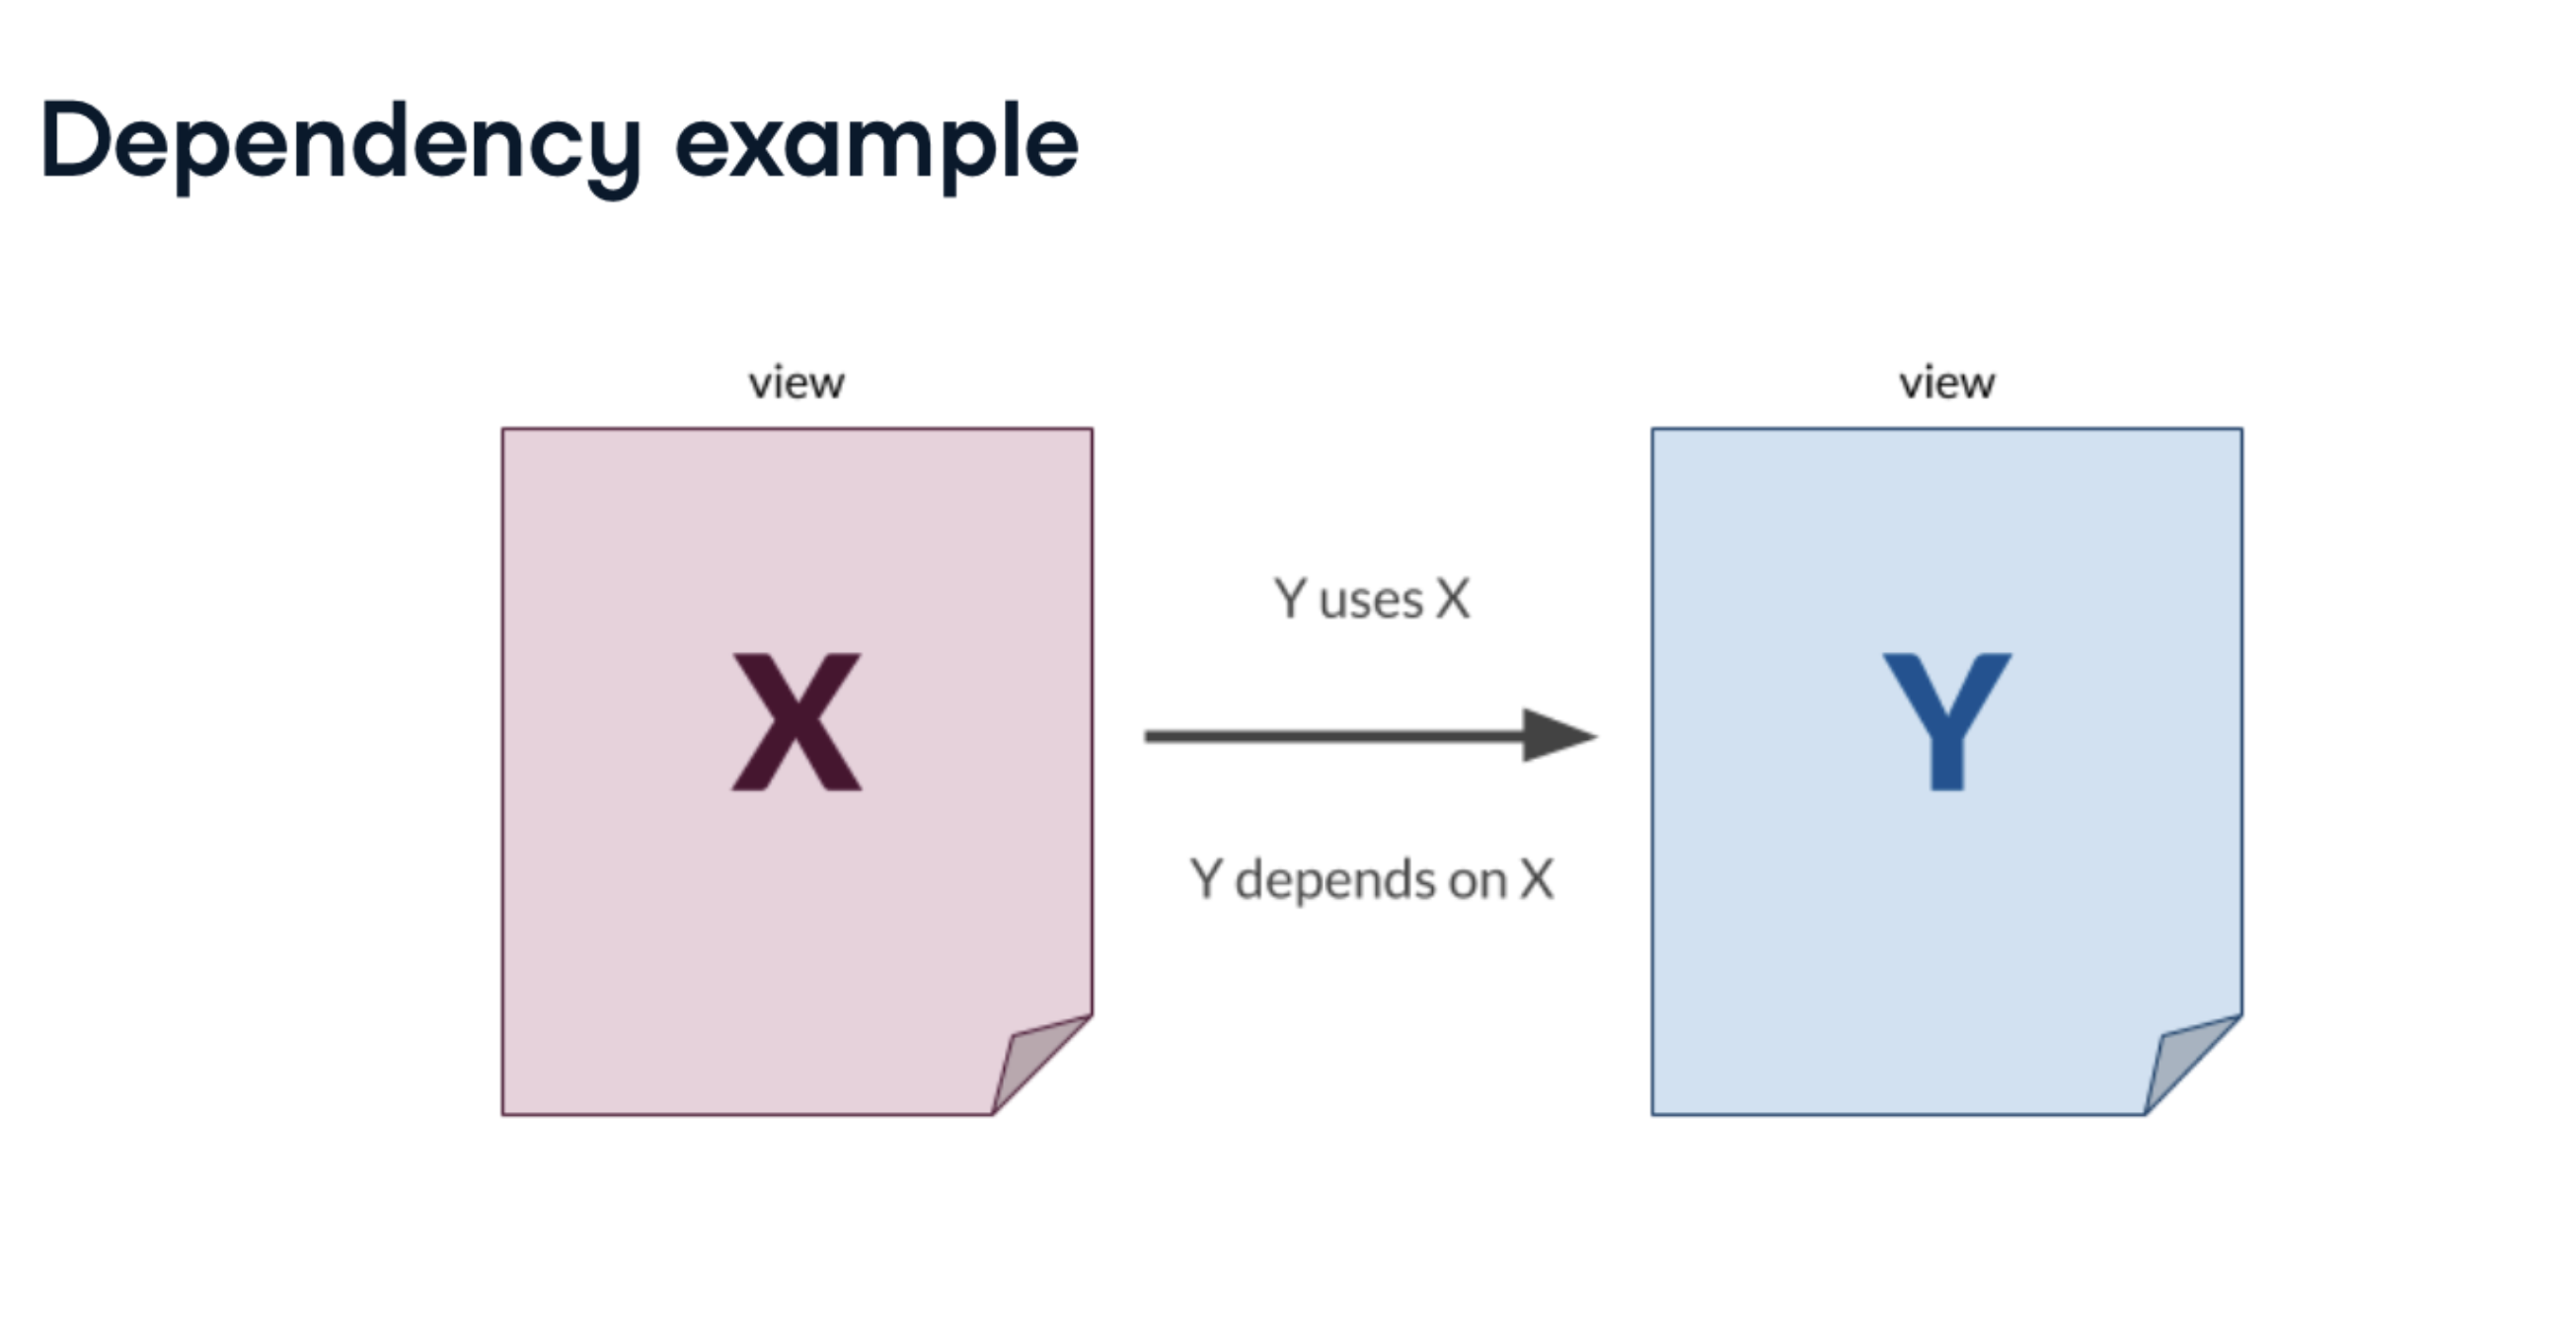
\includegraphics[width=1.0\textwidth]{figures/DependencyExample.png}
\end{figure}
\begin{itemize}
    \item Materialized views often depend on other materialized views
    \item In \ref{fig: Dependency example}, suppose that Y depends on X, but X deoesn't depends on Y and X has time consuming query. If Y refreshes before X refresh is complete, Y now has out-of-date data.
    \item This creates a \textbf{dependency chain} when refreshing views
    \item Not the most efficient to refresh all views at the same time.
\end{itemize}
\begin{figure}[H]
    \centering
    \caption{Tools for Dependency Management}
    \label{fig: Tools4DependeencyManagement}
    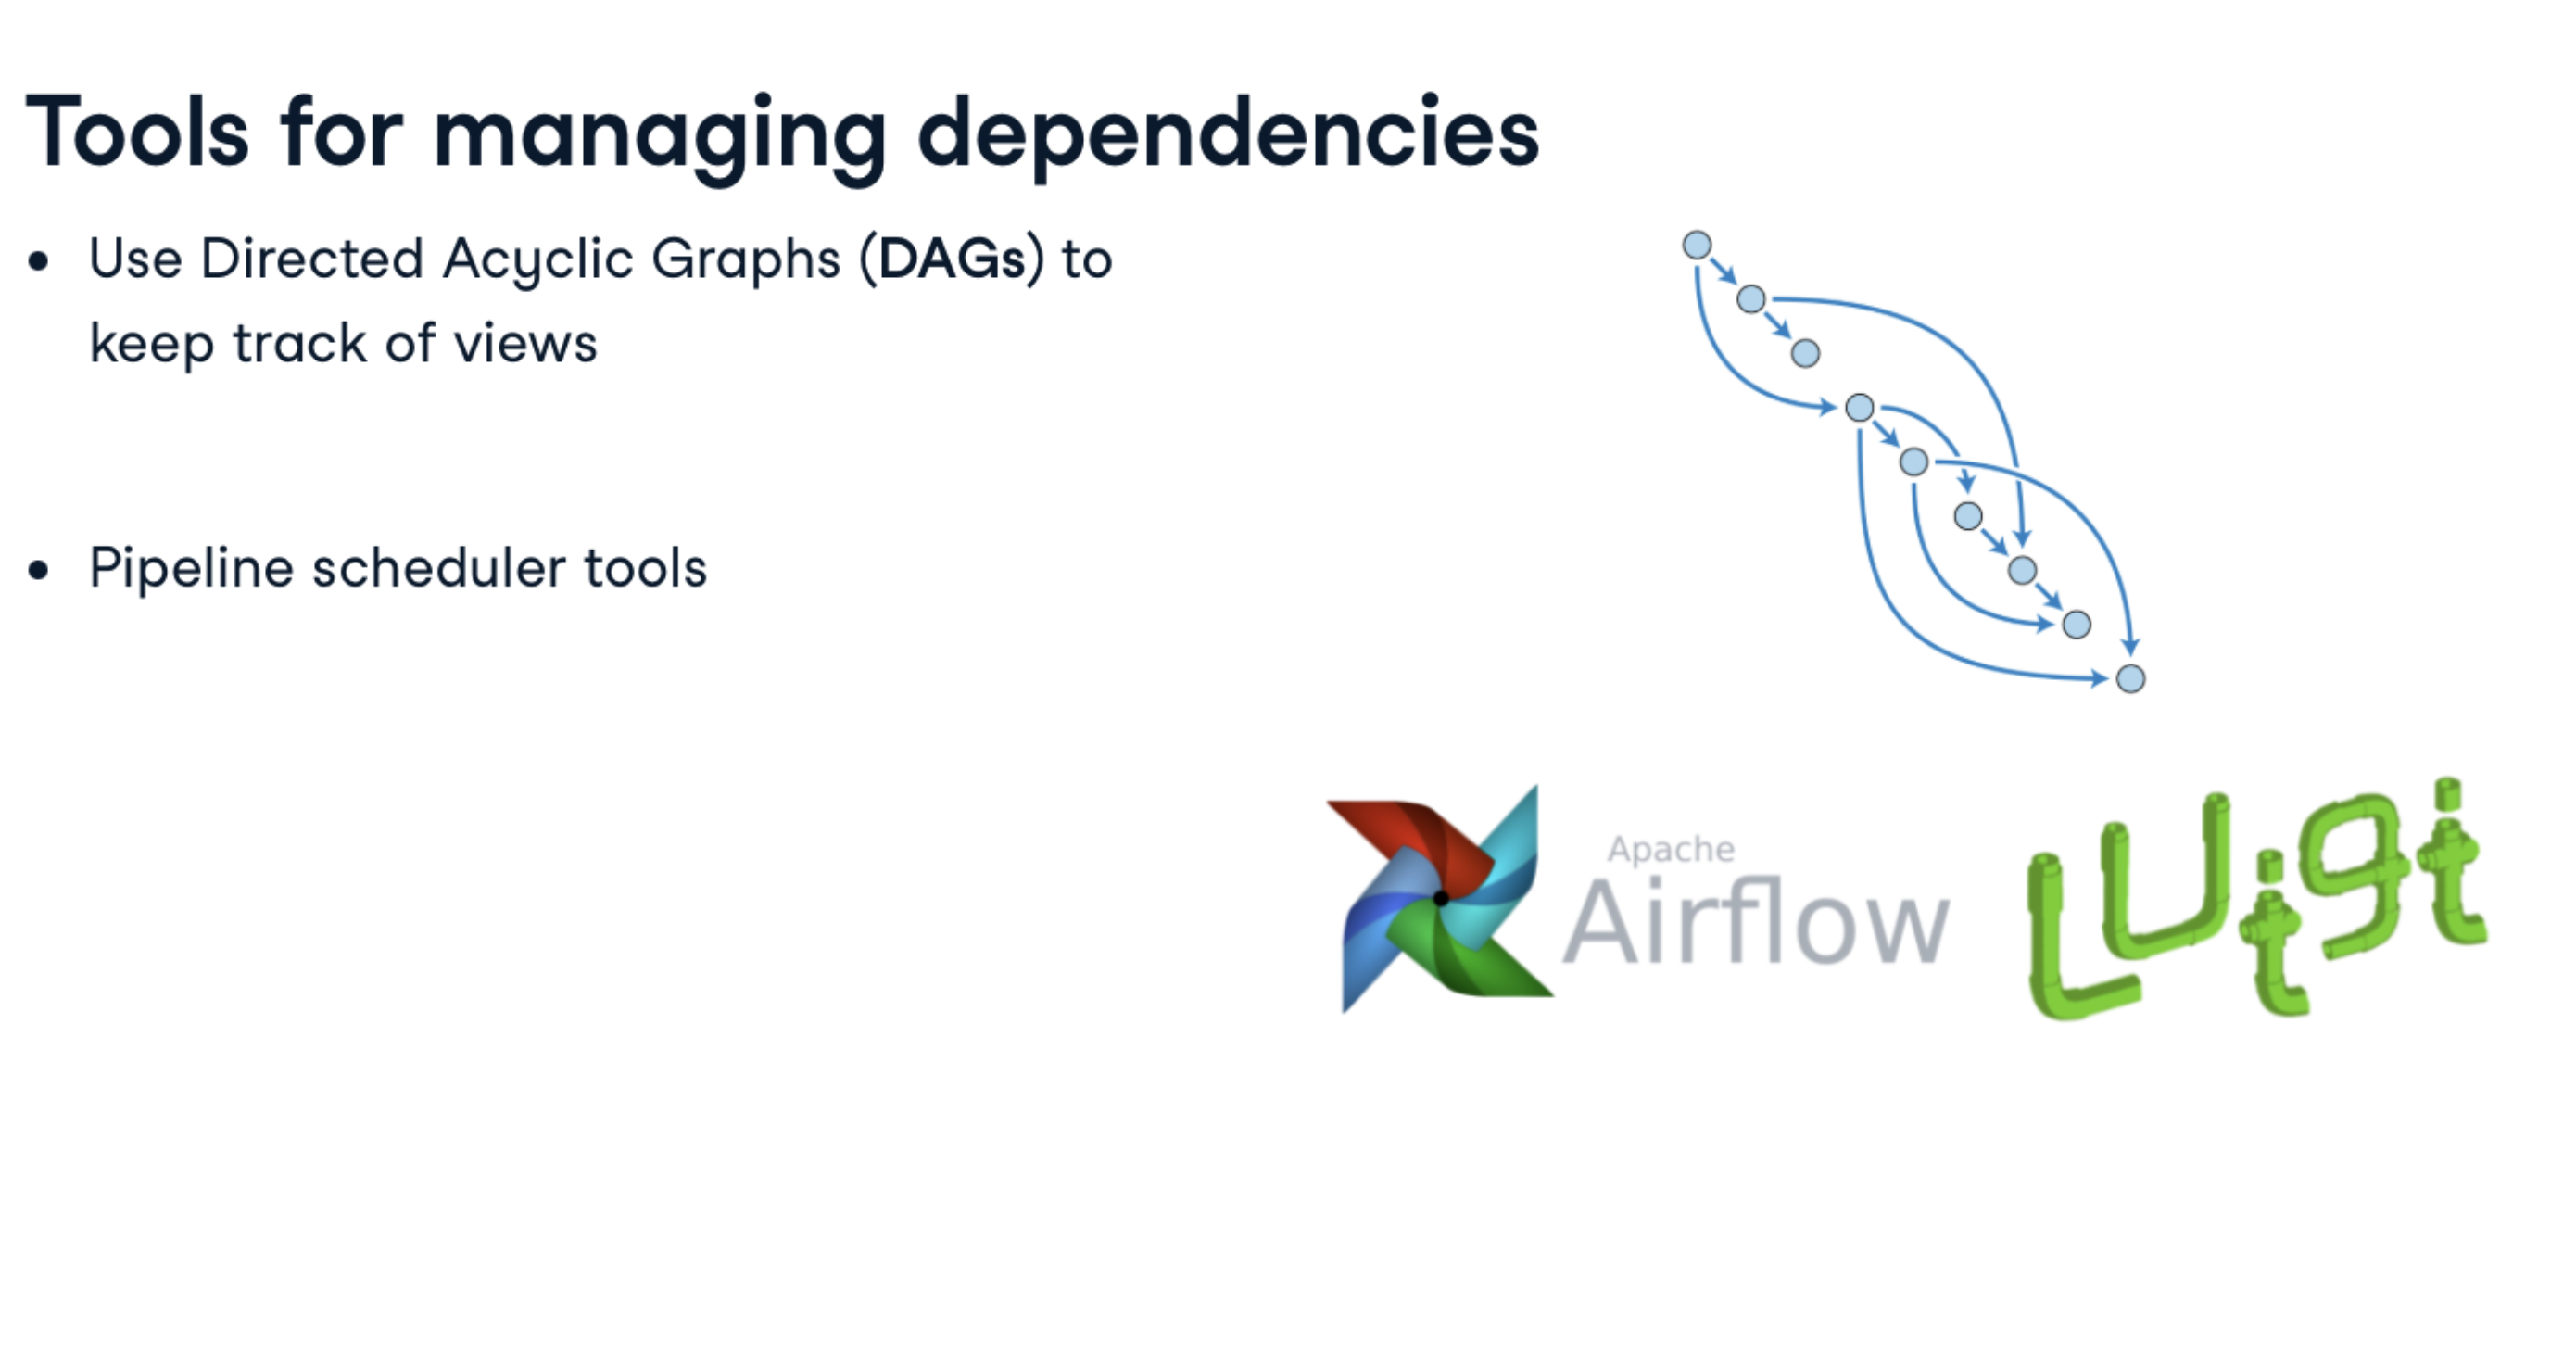
\includegraphics[width=1.0\textwidth]{figures/Tools4DependencyManagement.png}
\end{figure}

\section{Database Management}
\subsection{Database roles and access control}
\subsubsection{Database roles}
\begin{itemize}
    \item Manage database access permissions
    \item A database role is an entity that contains information that
    \begin{itemize}
        \item Define the role's Privileges
        \begin{itemize}
            \item Can you login?
            \item Can you create databases?
            \item Can you write to tables?
        \end{itemize}
        \item Interact with client authentication system
        \begin{itemize}
            \item Password
        \end{itemize}
    \end{itemize}
    \item Roles can be assigned to one or more users
    \item Roles are global across a database cluster installation
\end{itemize}

\subsubsection{Create a role}
\begin{itemize}
    \item Empty role
    \inputminted[
        firstline=85,
        lastline=85
    ]{SQL}{SQL/DatabaseDesign.sql}
    \item Roles with some attributes set
    \inputminted[
        firstline=87,
        lastline=91
    ]{SQL}{SQL/DatabaseDesign.sql}
\end{itemize}
\emph{Note: from https://www.postgresql.org/docs/current/role-attributes.html}

\subsubsection{GRANT and REVOKE privileges from roles}
\inputminted[
    firstline=95,
    lastline=99
]{SQL}{SQL/DatabaseDesign.sql}

The available privileges in PostgreSQL are:
\hl{SELECT}, \hl{INSERT}, \hl{UPDATE}, \hl{DELETE}, \hl{TRUNCATE}, \hl{REFERENCES}, \hl{TRIGGER}, \hl{CREATE},
\hl{CONNECT}, \hl{TEMPORARY}, \hl{EXECUTE}, and \hl{USAGE}.
\emph{NOTE: from https://www.postgresql.org/docs/current/ddl-priv.html}

\subsubsection{Users and groups (are both roles)}
\begin{itemize}
    \item A role is an entity that can function as a user and/or a group
    \begin{itemize}
        \item \textbf{Group roles}
        \inputminted[
            firstline=85,
            lastline=85
        ]{SQL}{SQL/DatabaseDesign.sql}
        \item \textbf{User roles}, here alex is an intern at a company until 2020-01-01 then
        \inputminted[
            firstline=87,
            lastline=87
        ]{SQL}{SQL/DatabaseDesign.sql}
        \inputminted[
            firstline=97,
            lastline=99
        ]{SQL}{SQL/DatabaseDesign.sql}
    \end{itemize}
\end{itemize}
\begin{figure}[H]
    \centering
    \caption{Roles}
    \label{fig:Role}
    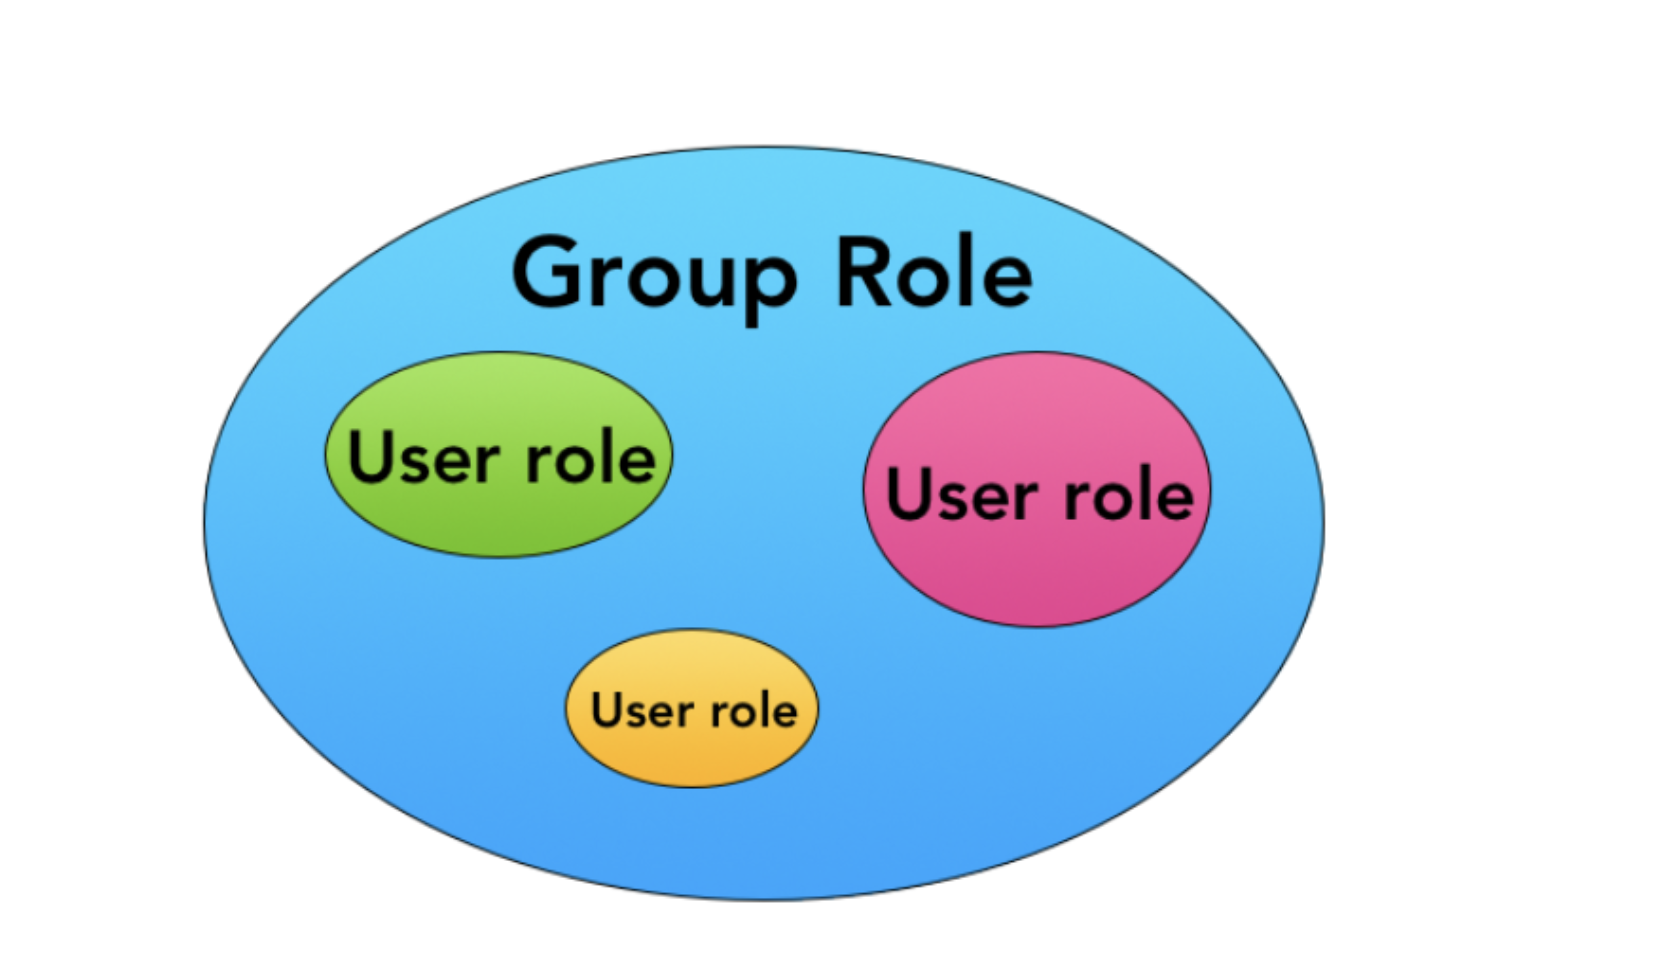
\includegraphics[width=1.0\textwidth]{figures/Roles.png}
\end{figure}

\begin{figure}[H]
    \centering
    \caption{Common PostgreSQL Roles}
    \label{fig:CommonDefaultRoles}
    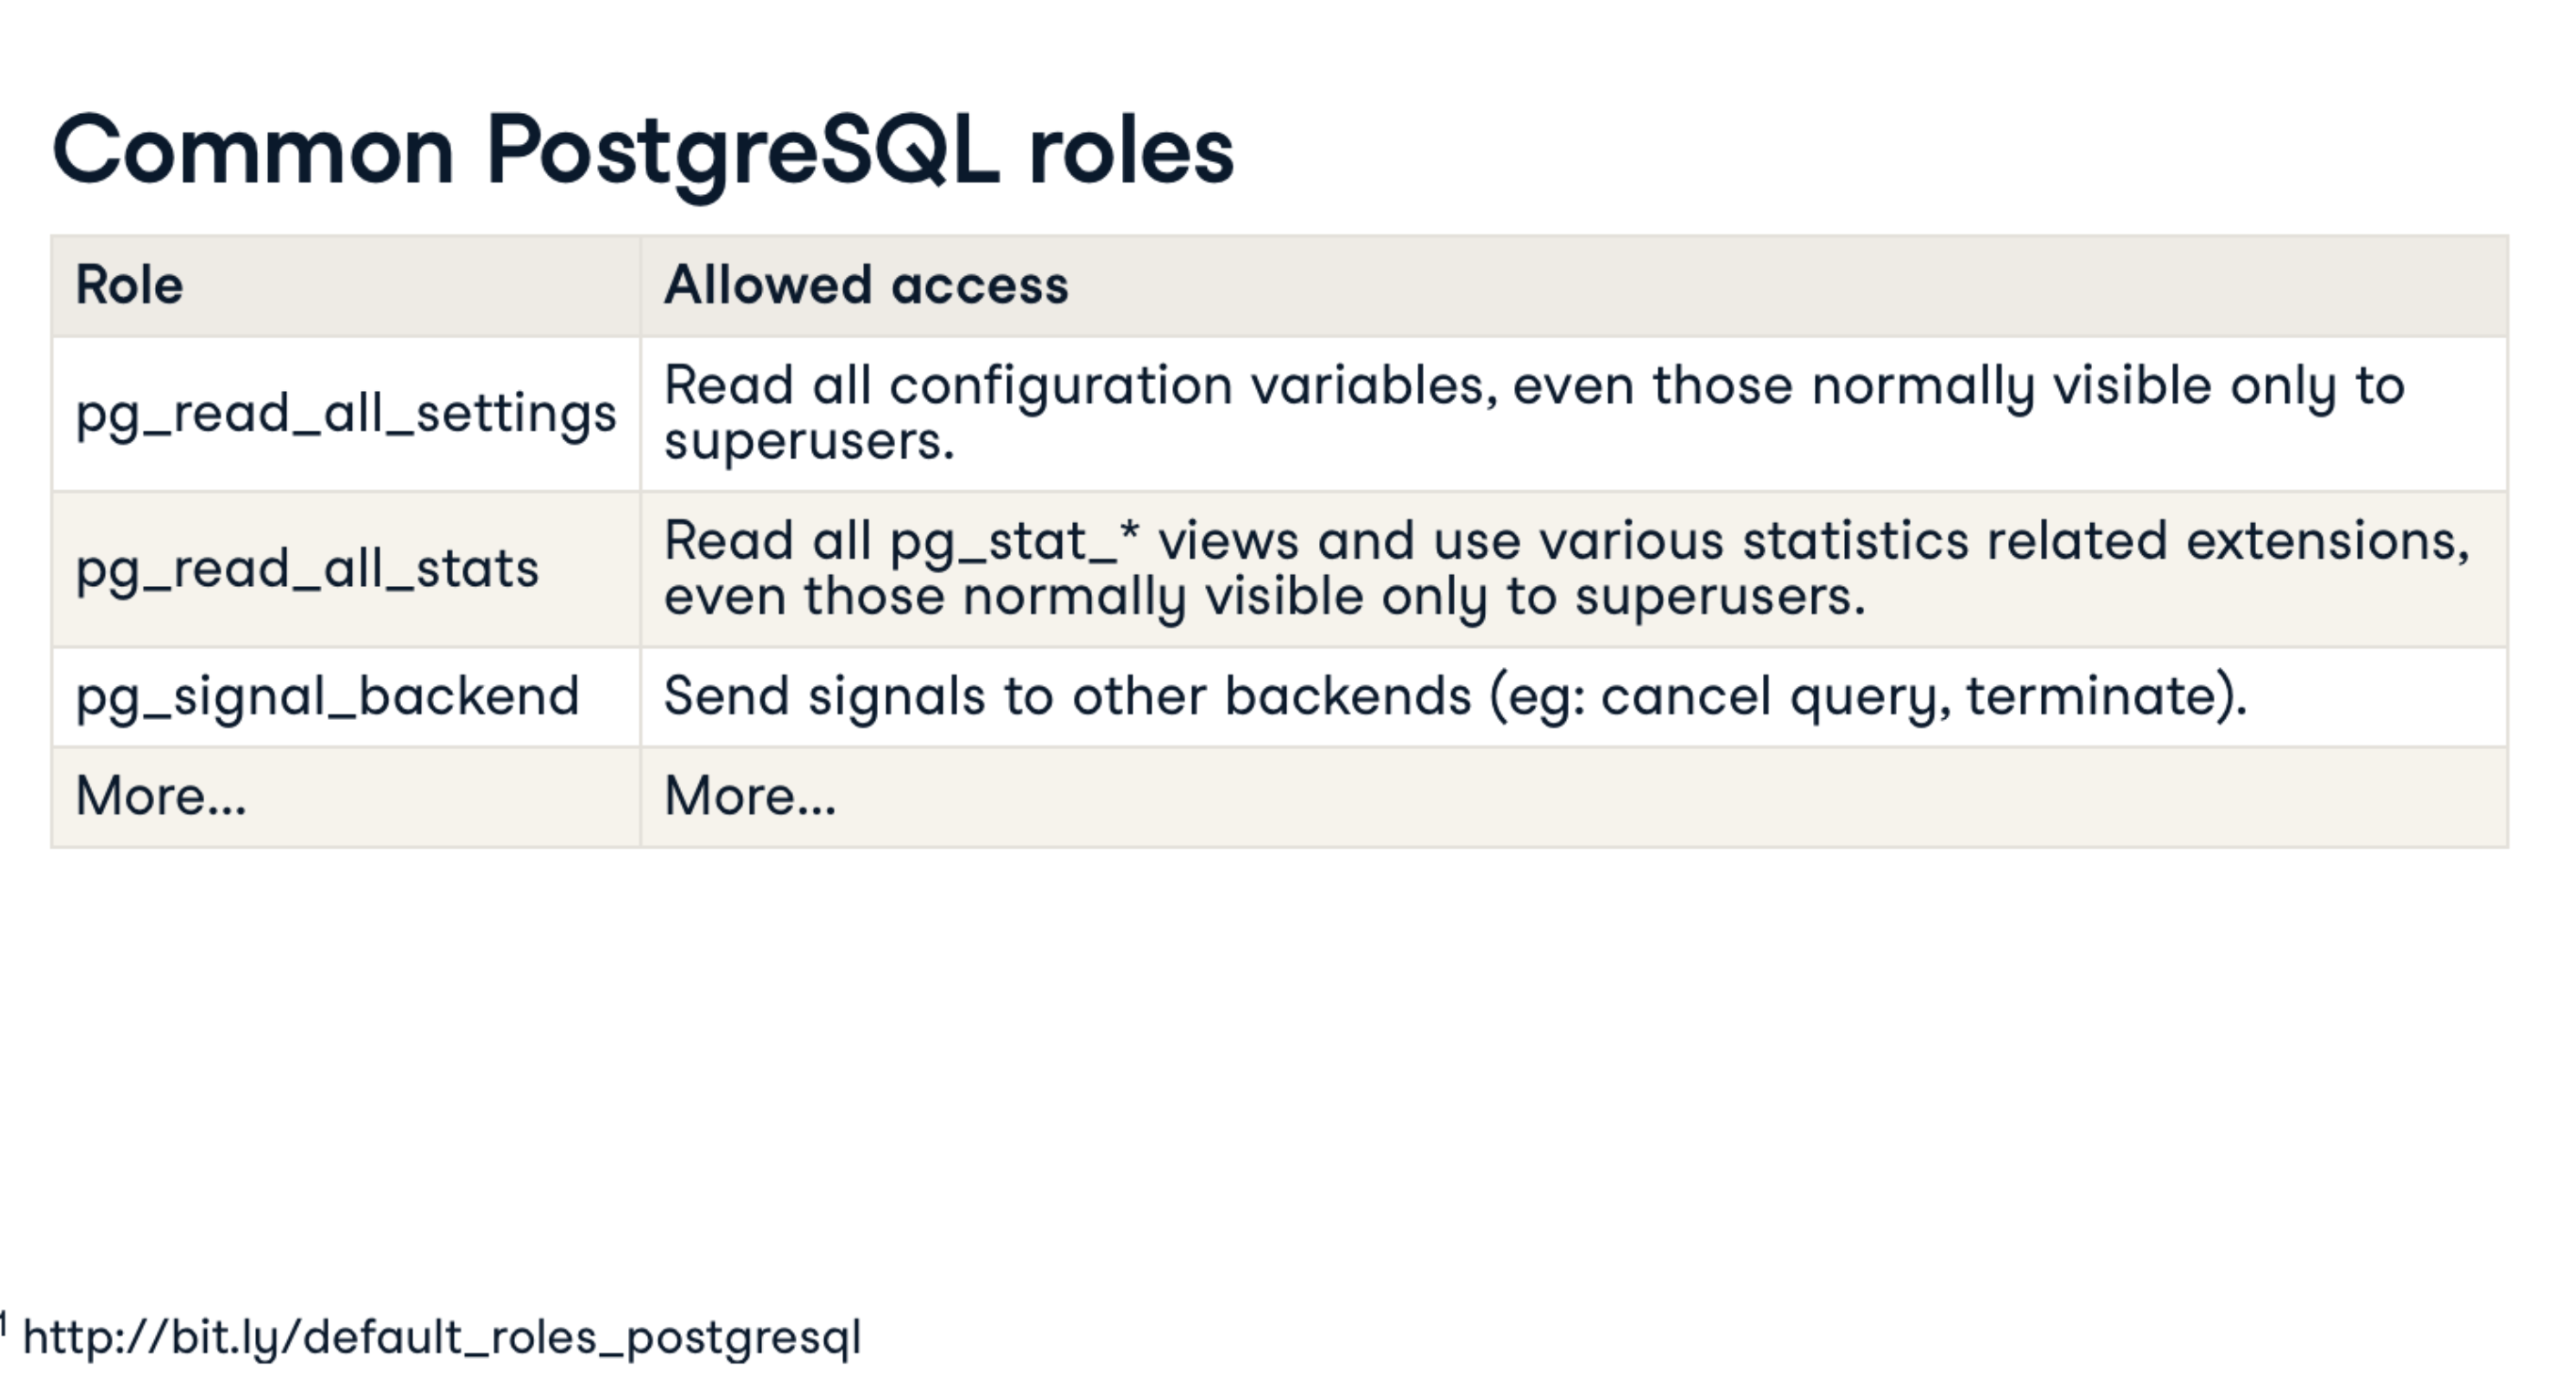
\includegraphics[width=1.0\textwidth]{figures/CommonDefaultRoles.png}
\end{figure}

\subsubsection{Benefit and pitfalls of roles}
\textbf{Benefits}
\begin{itemize}
    \item Roles live on after users are deleted
    \item Roles can be created before user accounts
    \item Save DBAa time
\end{itemize}
\textbf{Pitfalls}
\begin{itemize}
    \item Sometimes a role gives a specific user too much Access
    \begin{itemize}
        \item You need to pay attention
    \end{itemize}
\end{itemize}

\subsection{Table partitioning}
\subsubsection{Why partition?}
Tables grow (100s Gb / Tb)
\textbf{Problem:} queries/updates becomes slower \\
\textbf{Because:} e.g., indices don't fit memory \\
\textbf{Solution:} split table into smaller parts (=\textbf{partitioning})

\subsubsection{Data modeling refresher}
\begin{enumerate}
    \item Conceptual data model
    \item Logical data model \\
    For partitioning, logical model is the same
    \item Physical data model \\
    Partitioning is part of physical data model
\end{enumerate}

\subsubsection{Vertical partitioning}
\begin{figure}[H]
    \centering
    \caption{Vertical Partitioning}
    \label{fig:VerticalPartitioning}
    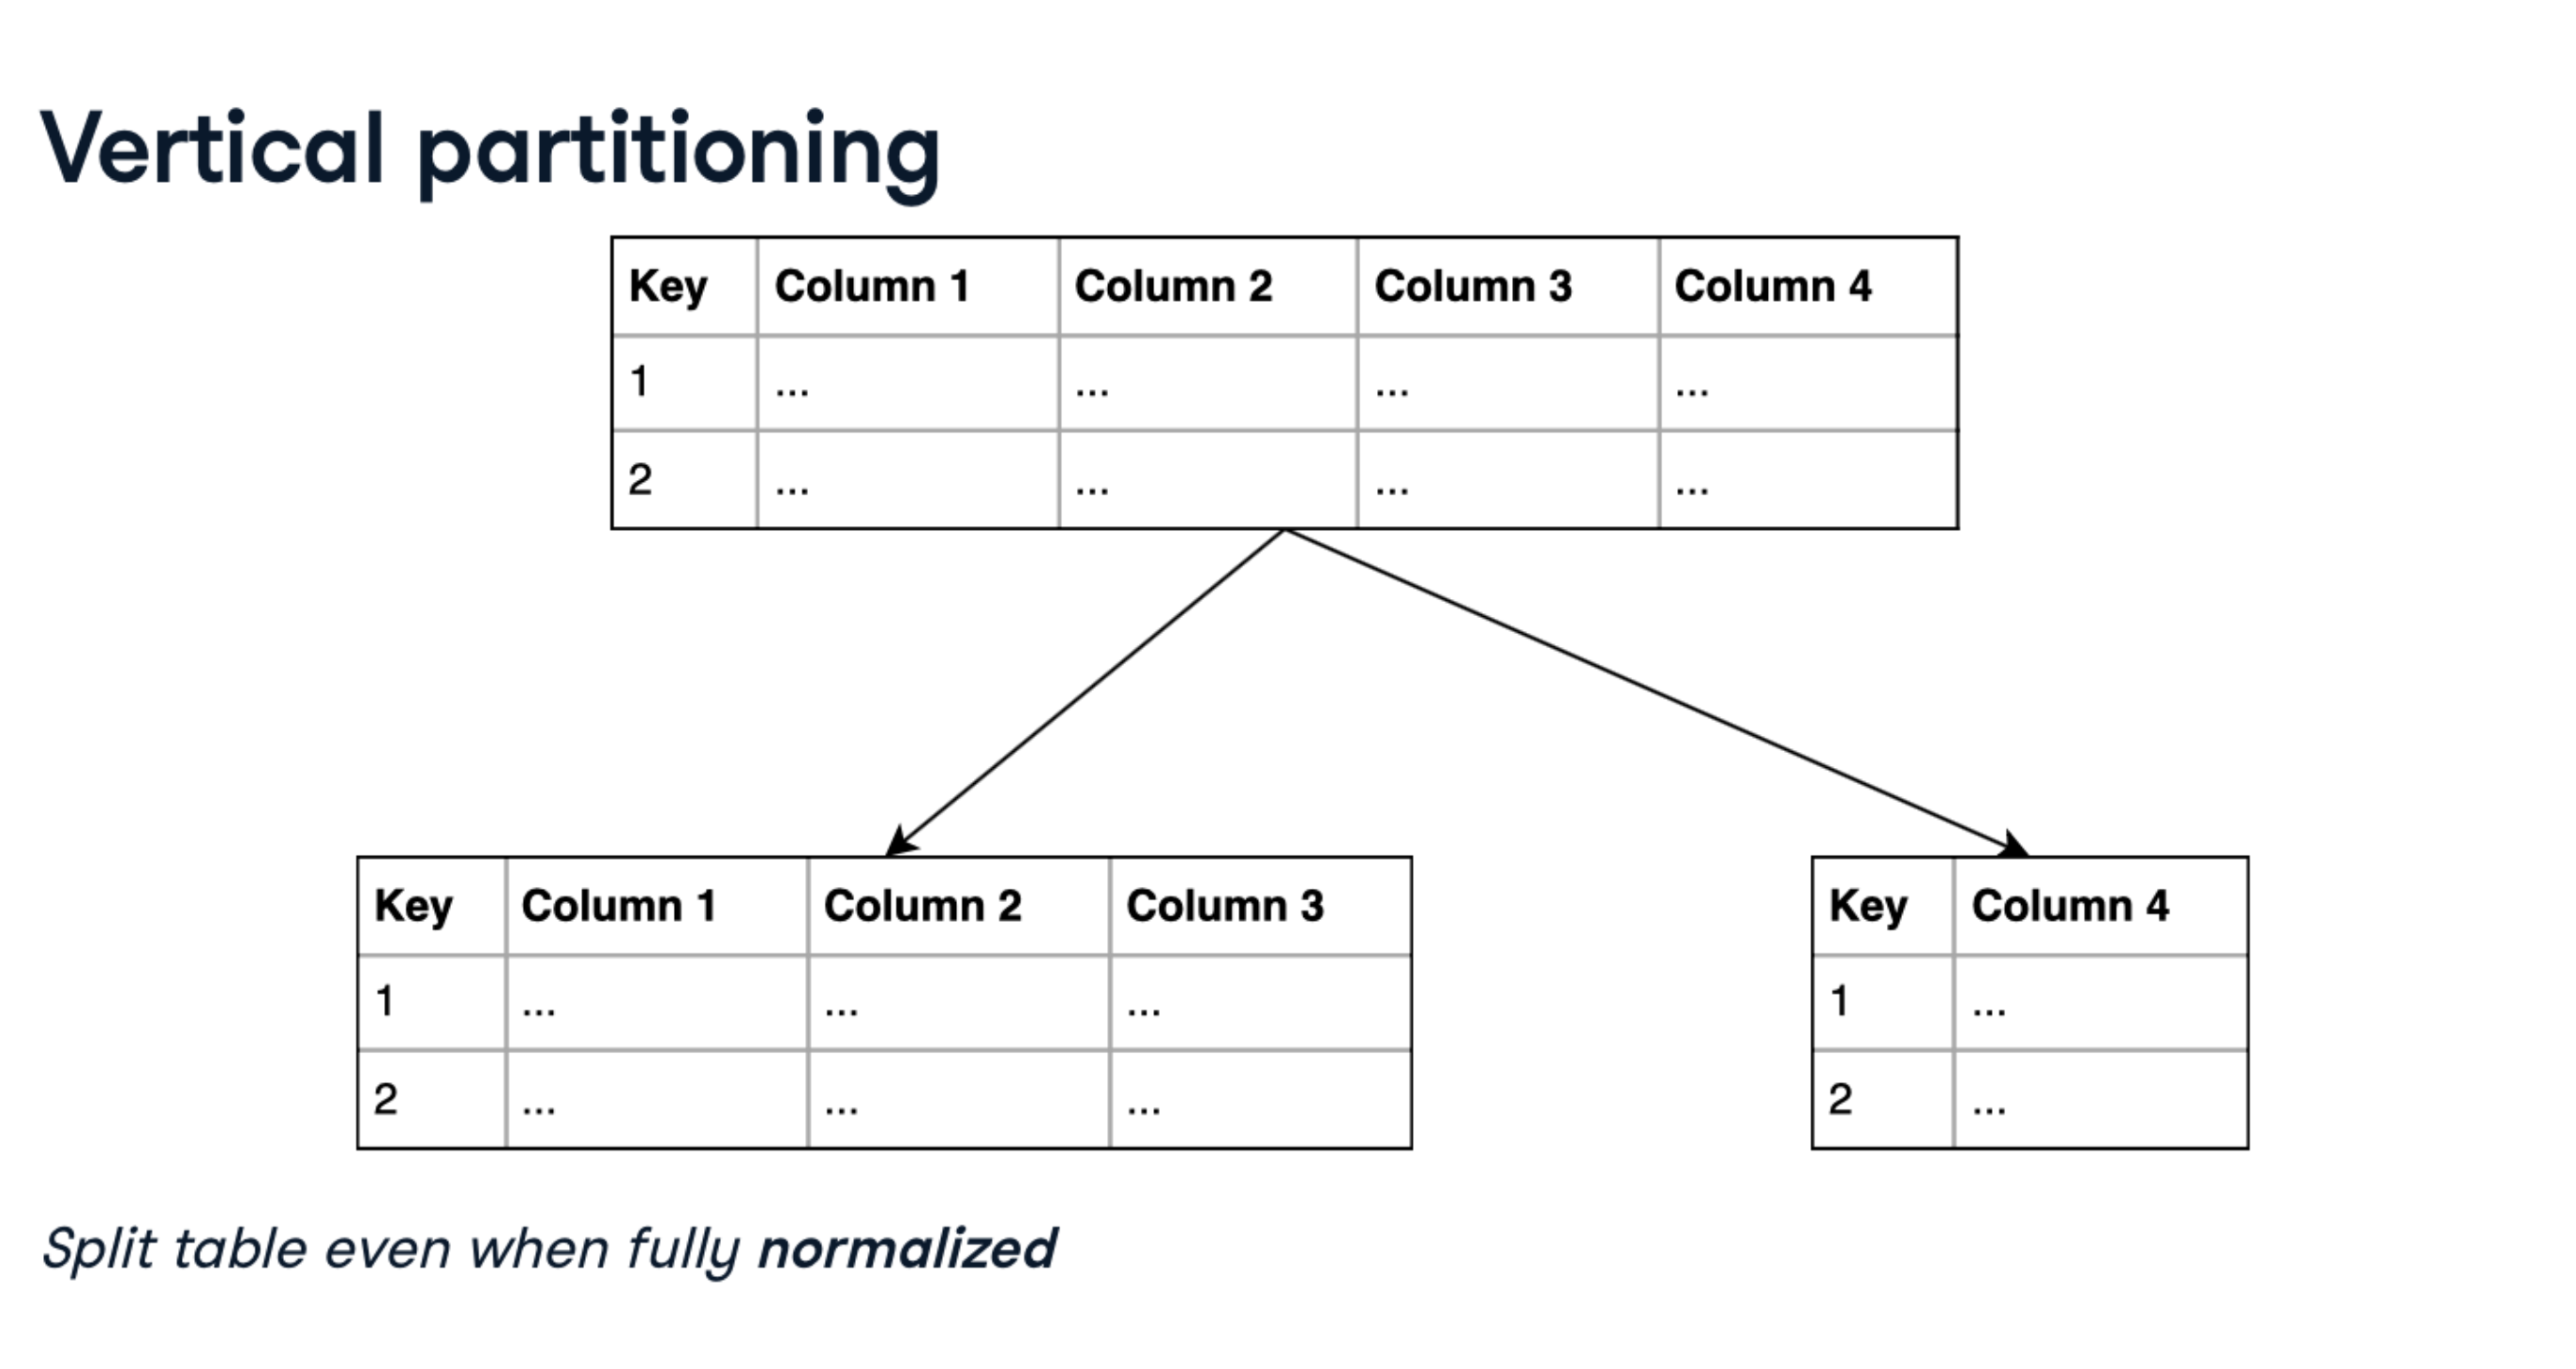
\includegraphics[width=1.0\textwidth]{figures/VerticalPartitioning.png}
\end{figure}

\begin{figure}[H]
    \centering
    \caption{Vertical Partitioning Example}
    \label{fig:VerticalPartitioningExample}
    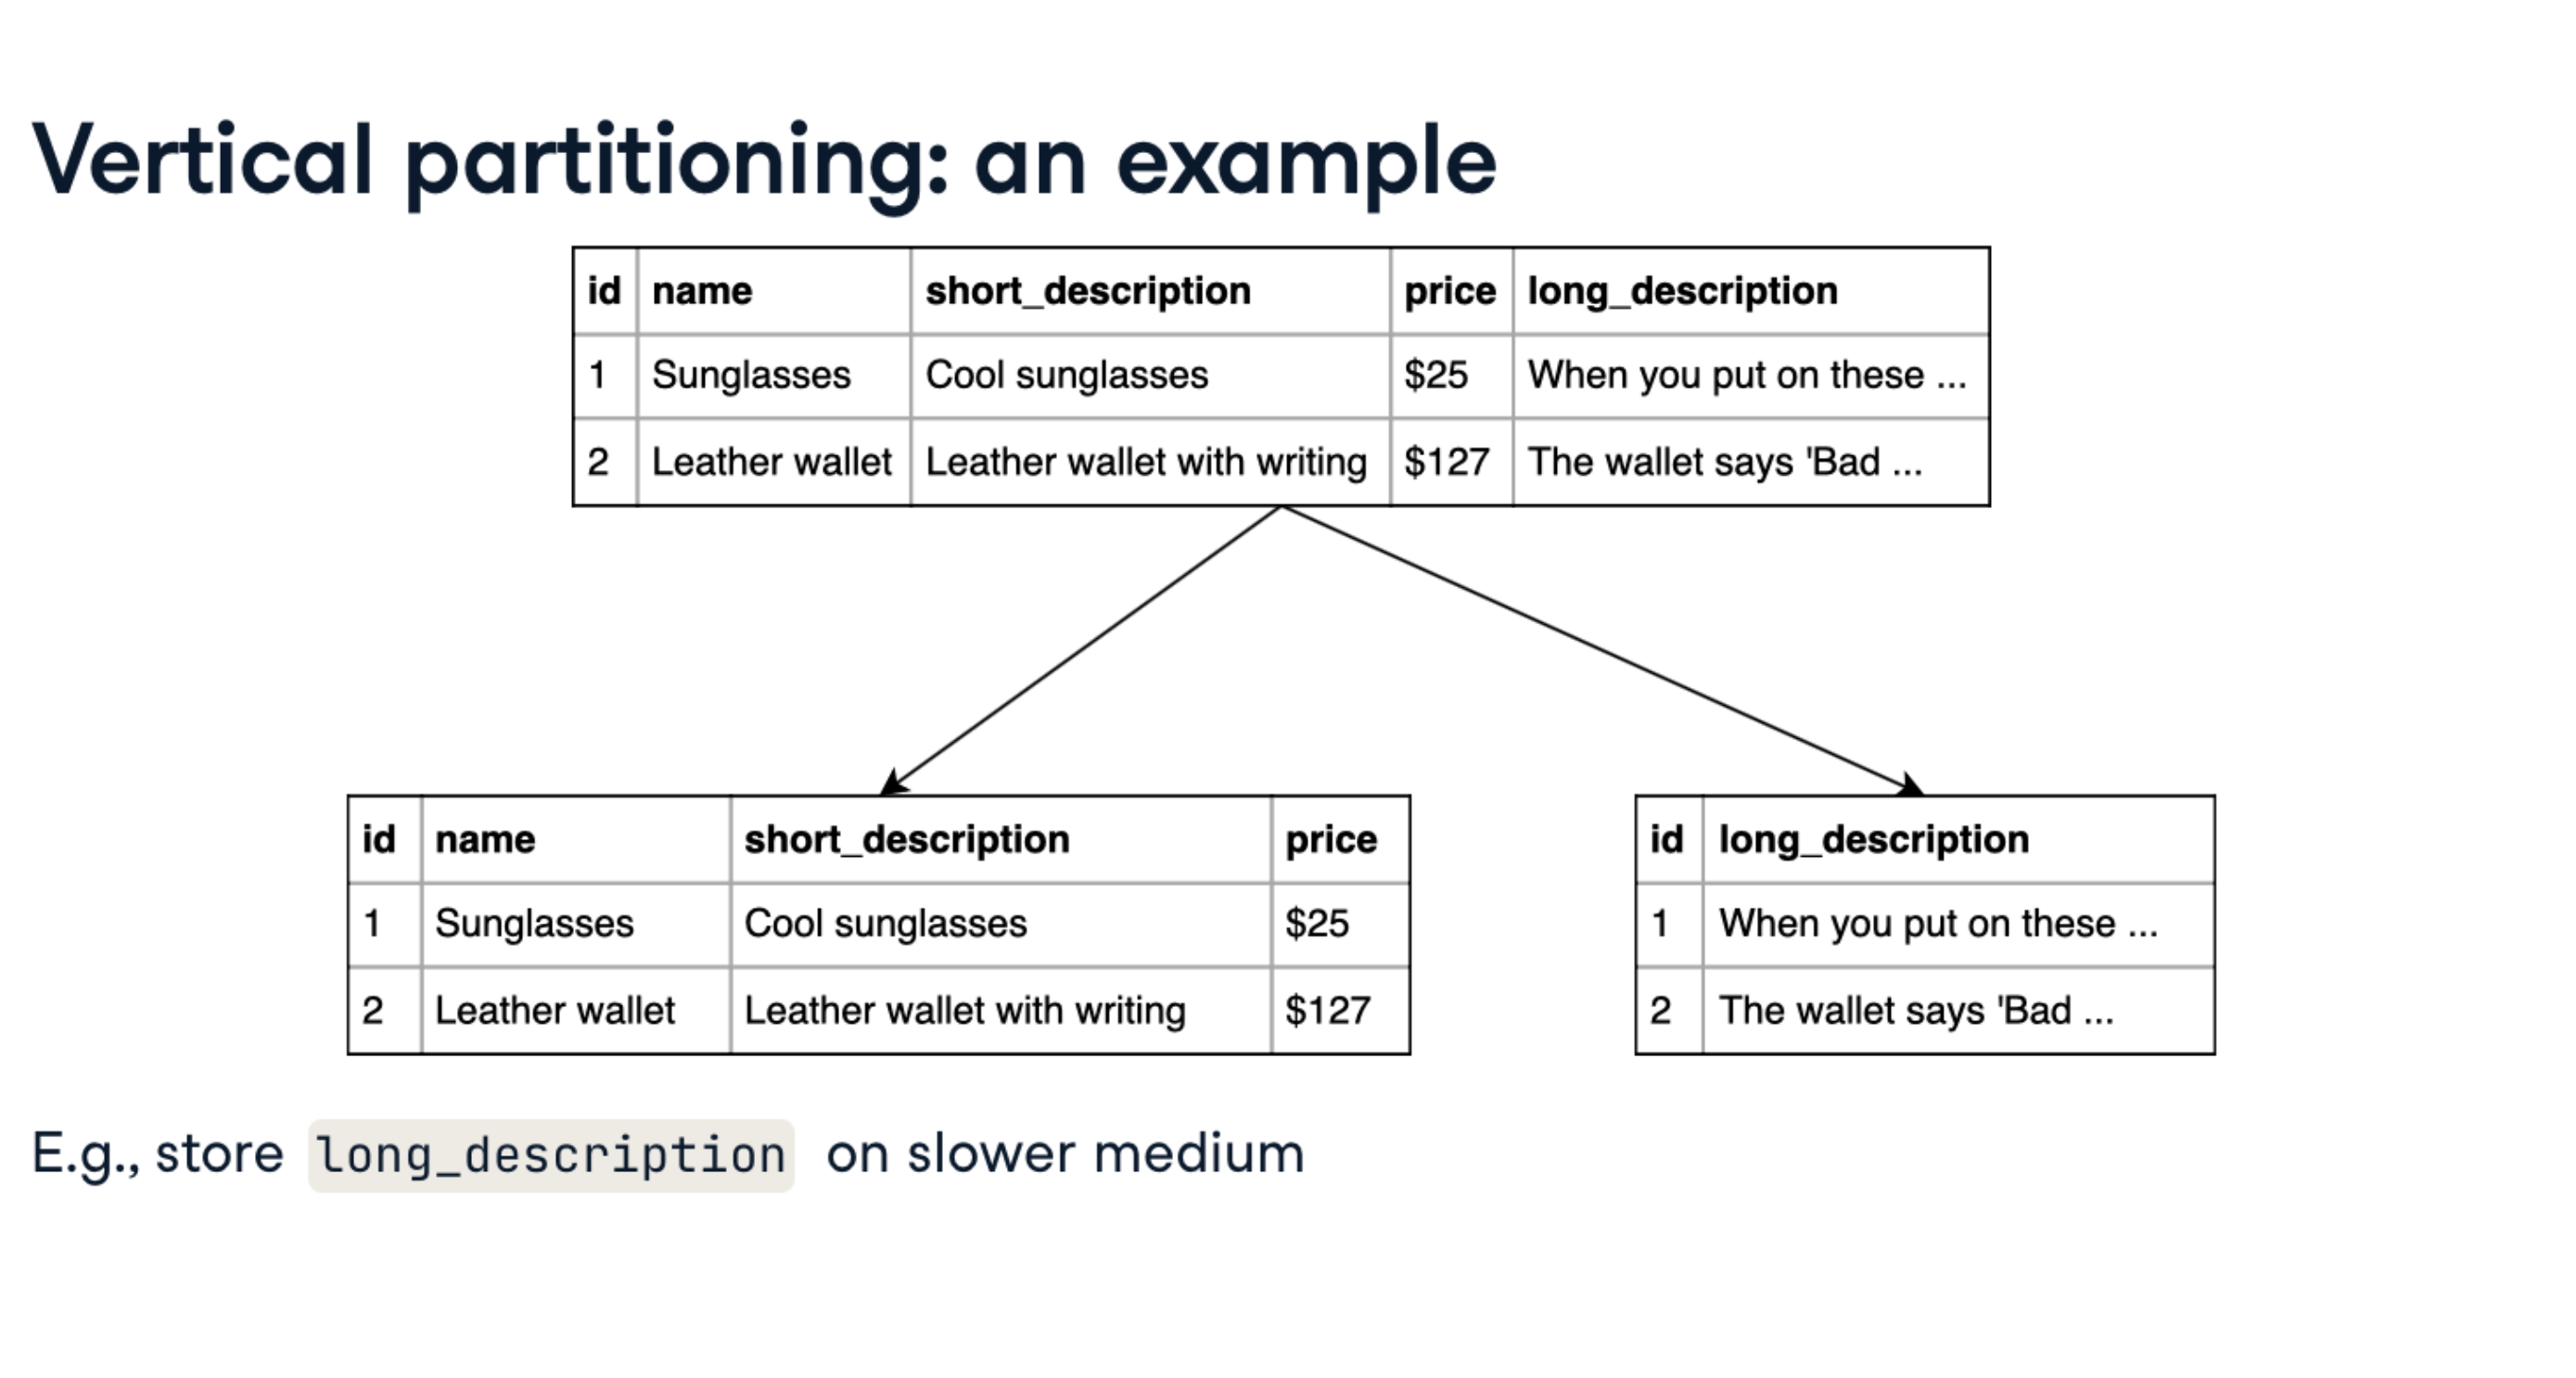
\includegraphics[width=1.0\textwidth]{figures/VPExample.png}
\end{figure}

\subsubsection{Horizontal Partitioning}
\begin{figure}[H]
    \centering
    \caption{Horizontal Partitioning}
    \label{fig:HPExample1}
    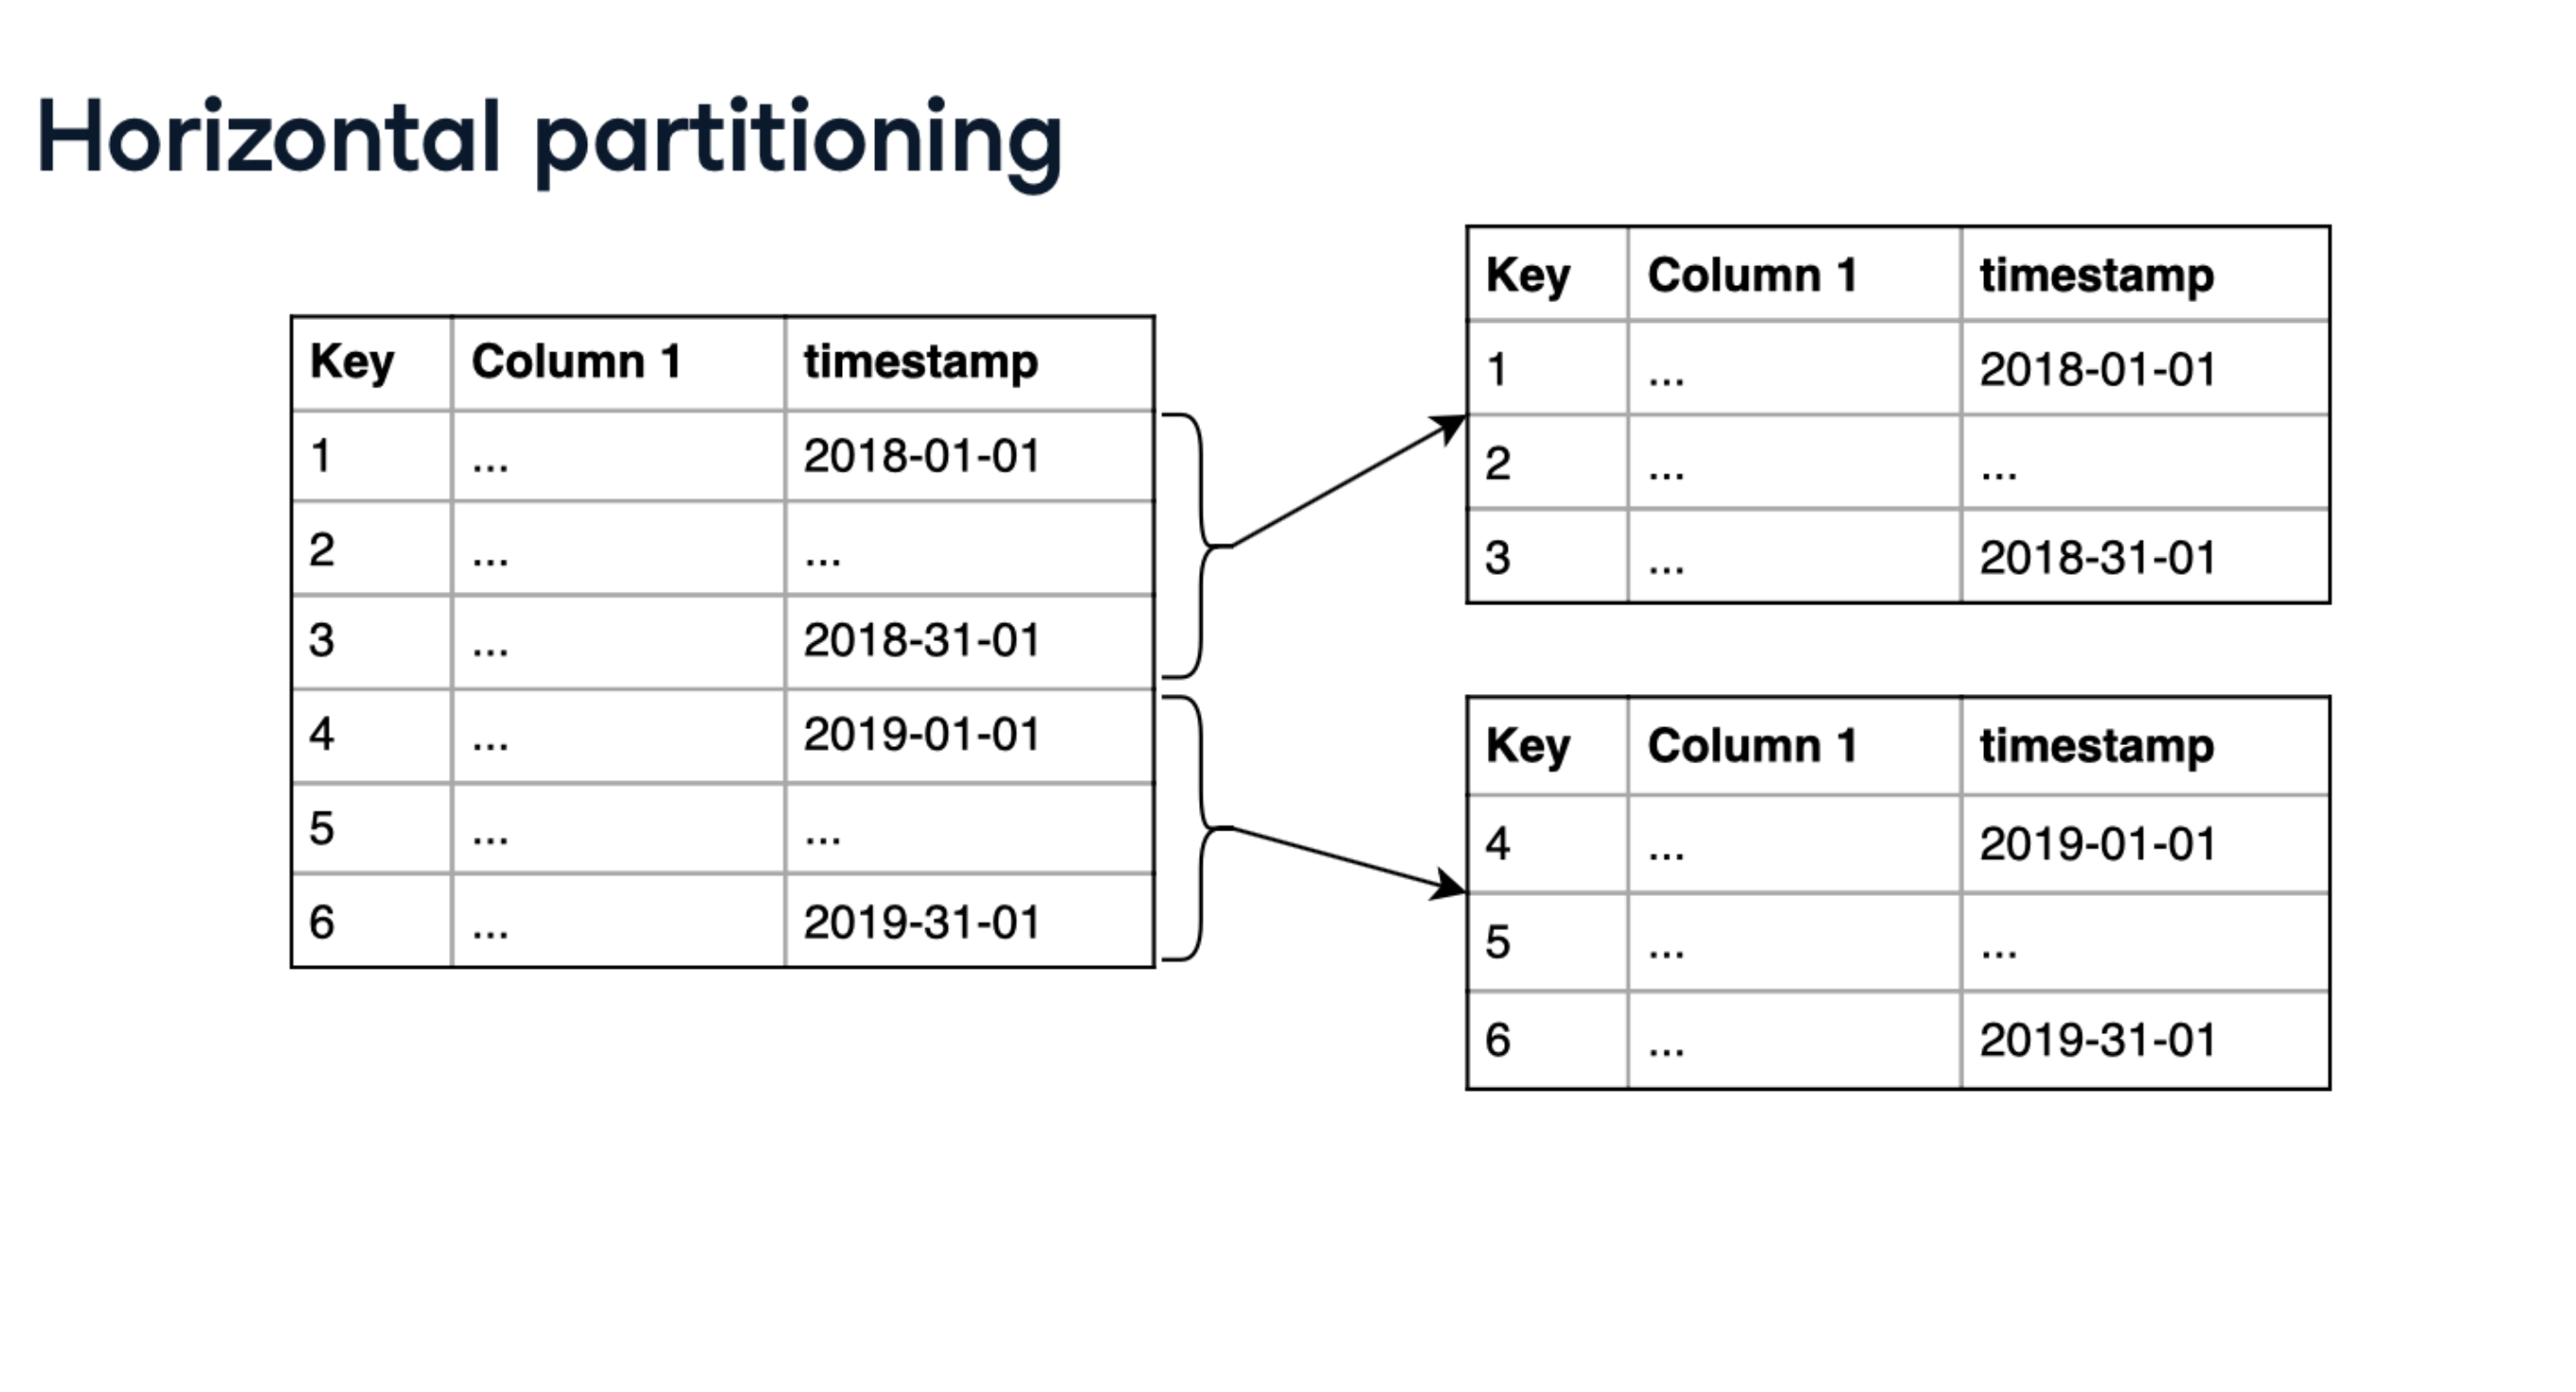
\includegraphics[width=1.0\textwidth]{figures/HPExample1.png}
\end{figure}

\begin{figure}[H]
    \centering
    \caption{Horizontal Partitioning Example}
    \label{fig:HPExample2}
    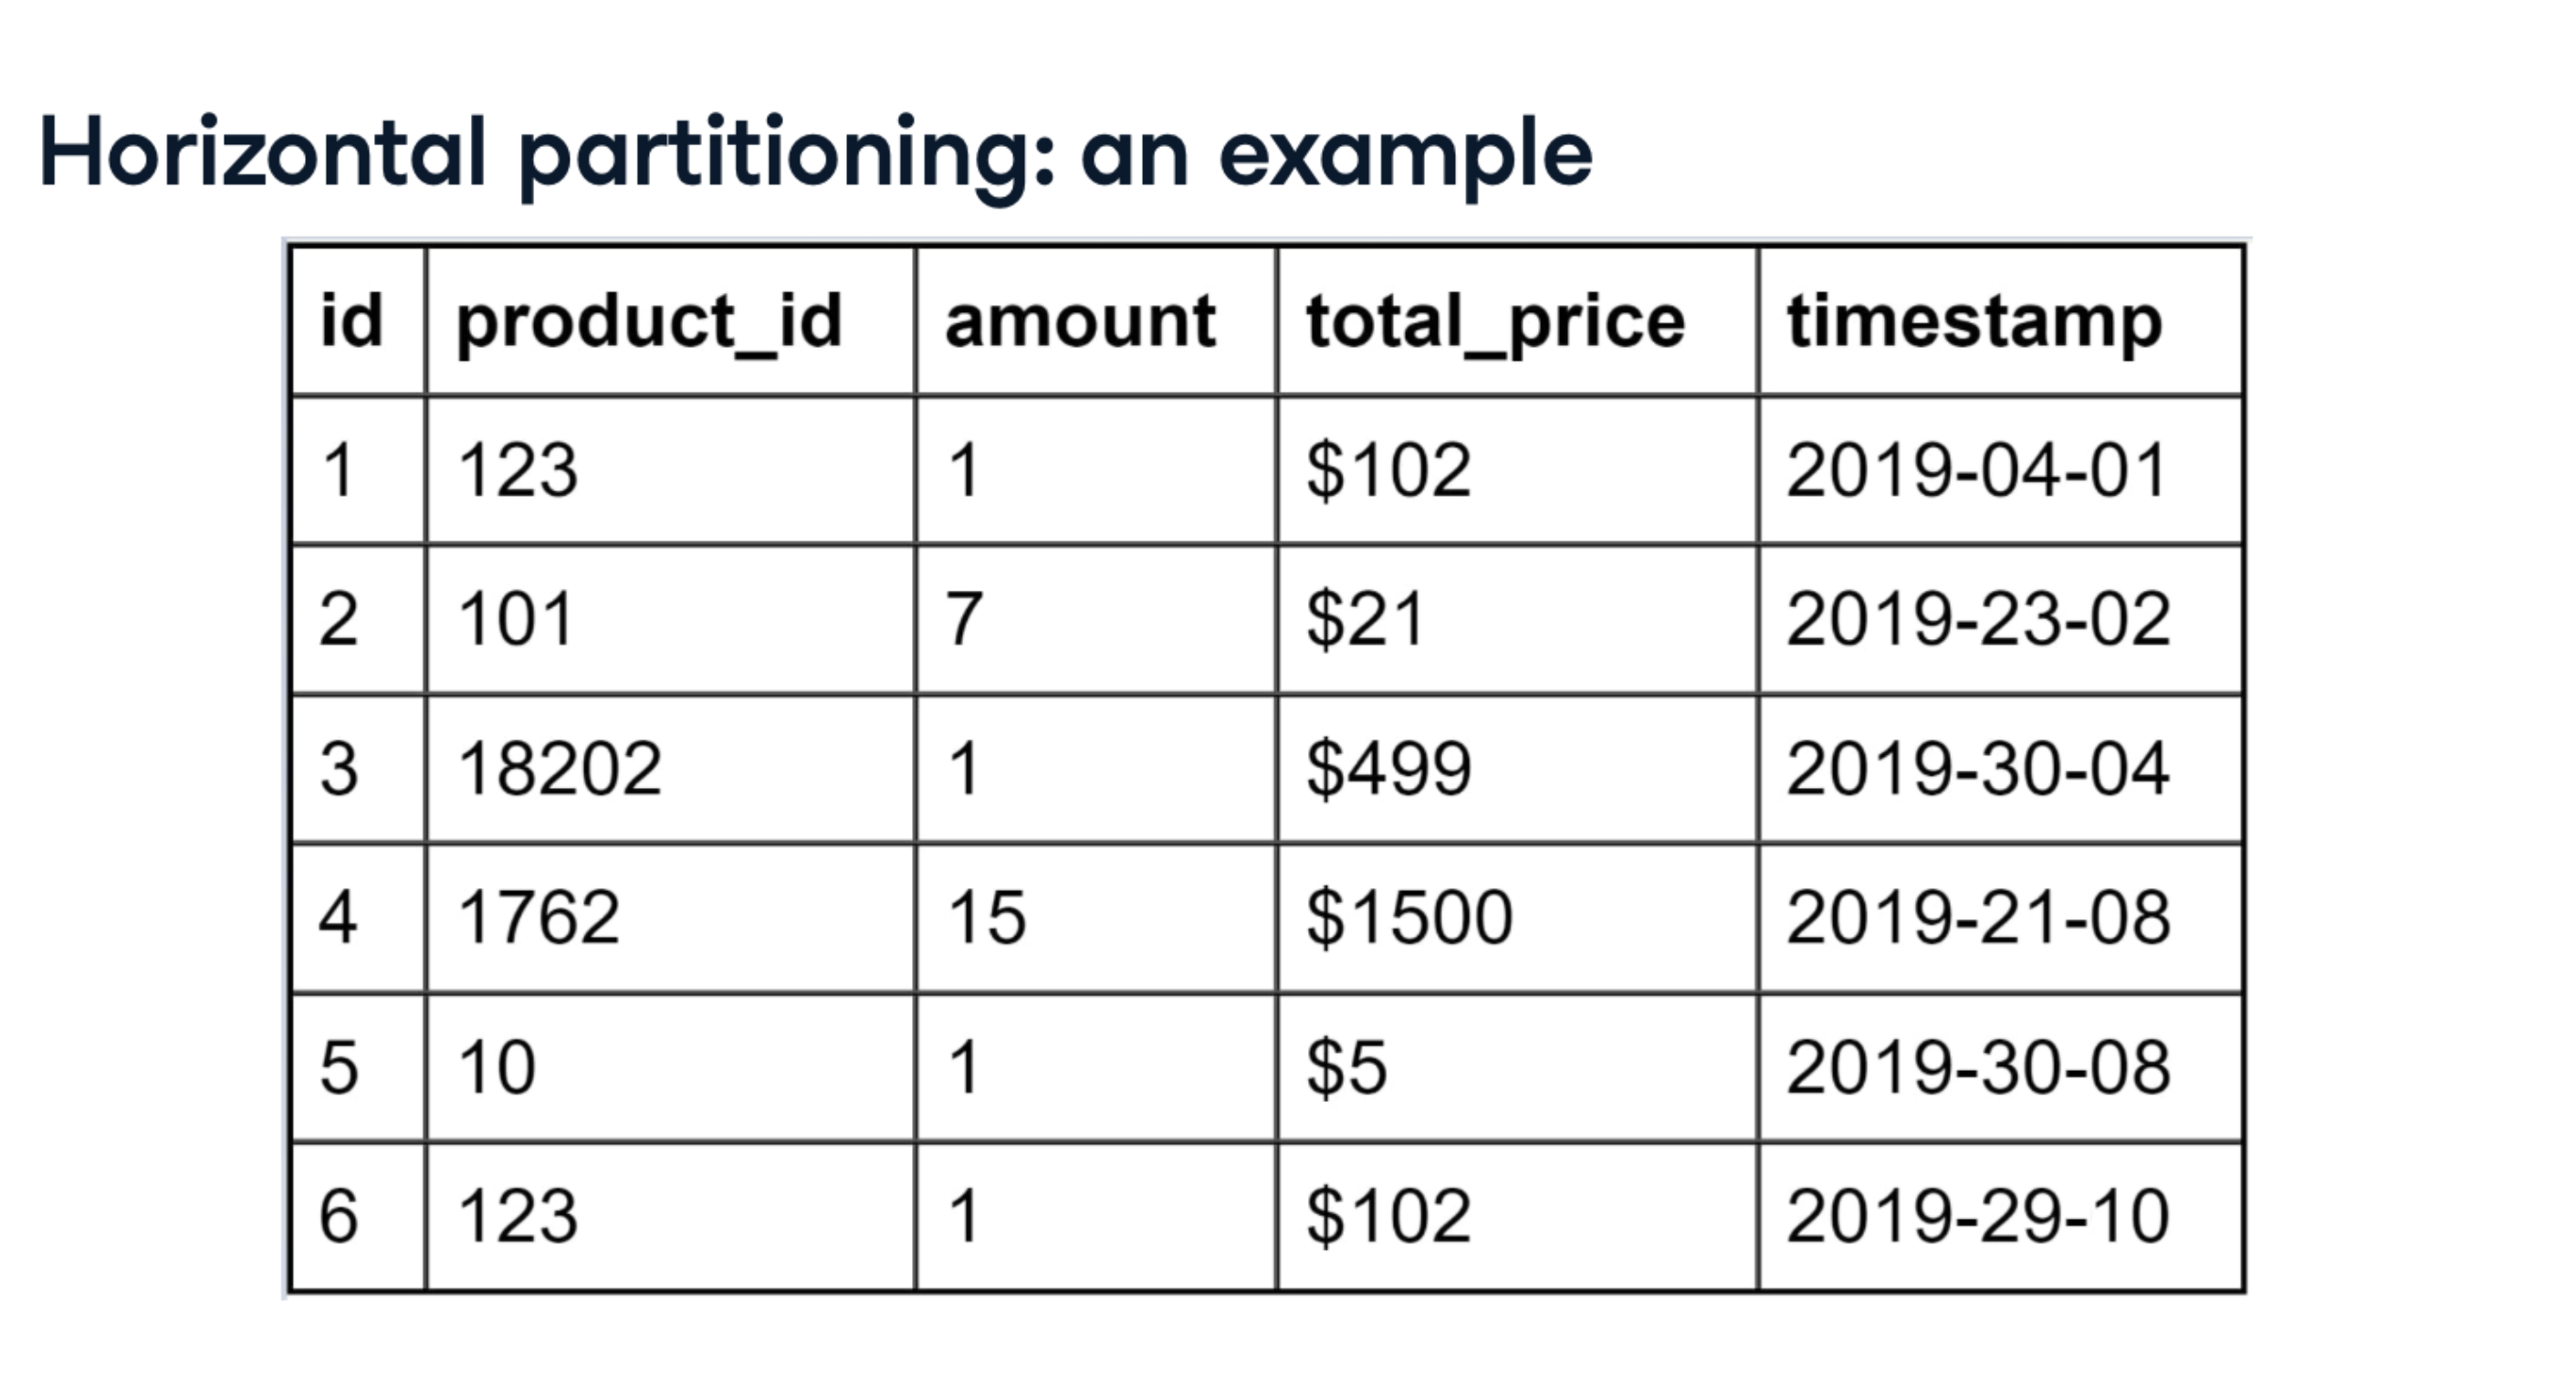
\includegraphics[width=1.0\textwidth]{figures/HPExample2.png}
\end{figure}

\begin{figure}[H]
    \centering
    \caption{Horizontal Partitioning Example}
    \label{fig:HPExample3}
    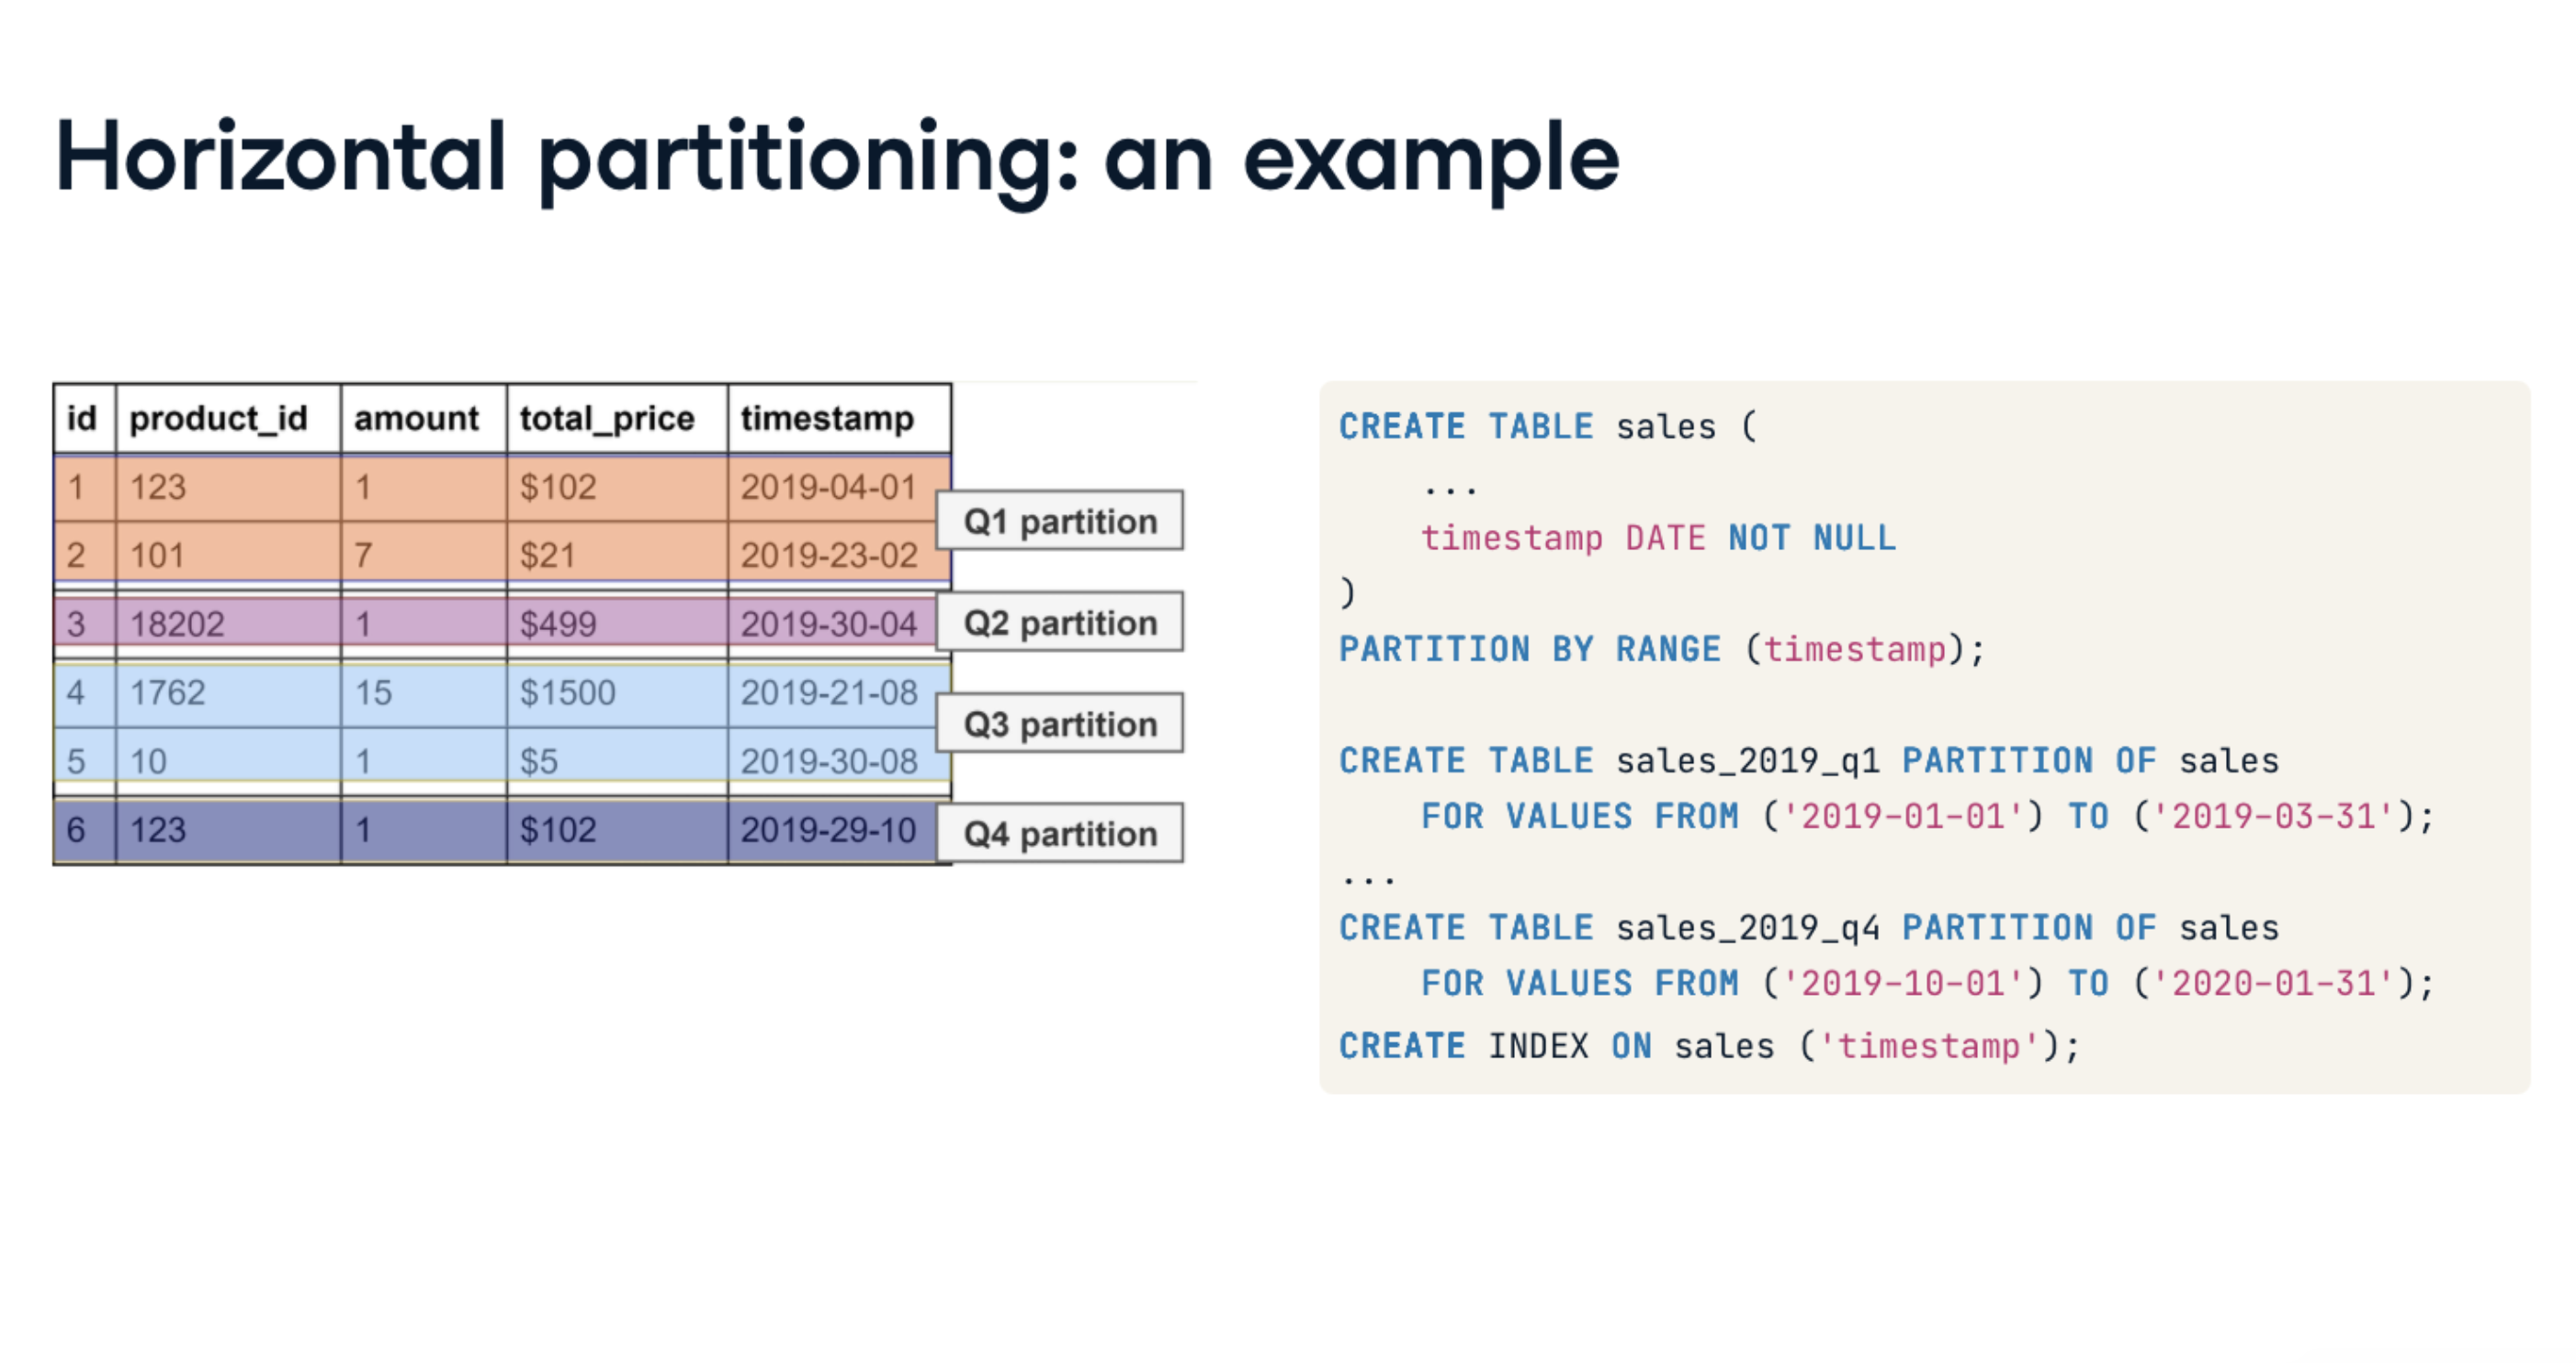
\includegraphics[width=1.0\textwidth]{figures/HPExample3.png}
\end{figure}

\subsubsection{Pros/cons of horizontal partitioning}
\textbf{Pros}
\begin{itemize}
    \item Indices of \textbf{heavily-used partitions} fit in memory
    \item Move to \textbf{specific medium}: slower vs faster
    \item Used for both OLAP and OLTP
\end{itemize}

\textbf{Cons}
\begin{itemize}
    \item Partitioning \textbf{existing table} can be a hassle
    \item Some \textbf{constraints} can not be set
\end{itemize}

When horizontal partitioning is applied to spread table over several machines, it's called sharding.
\begin{figure}[H]
    \centering
    \caption{Sharding}
    \label{fig:Sharding}
    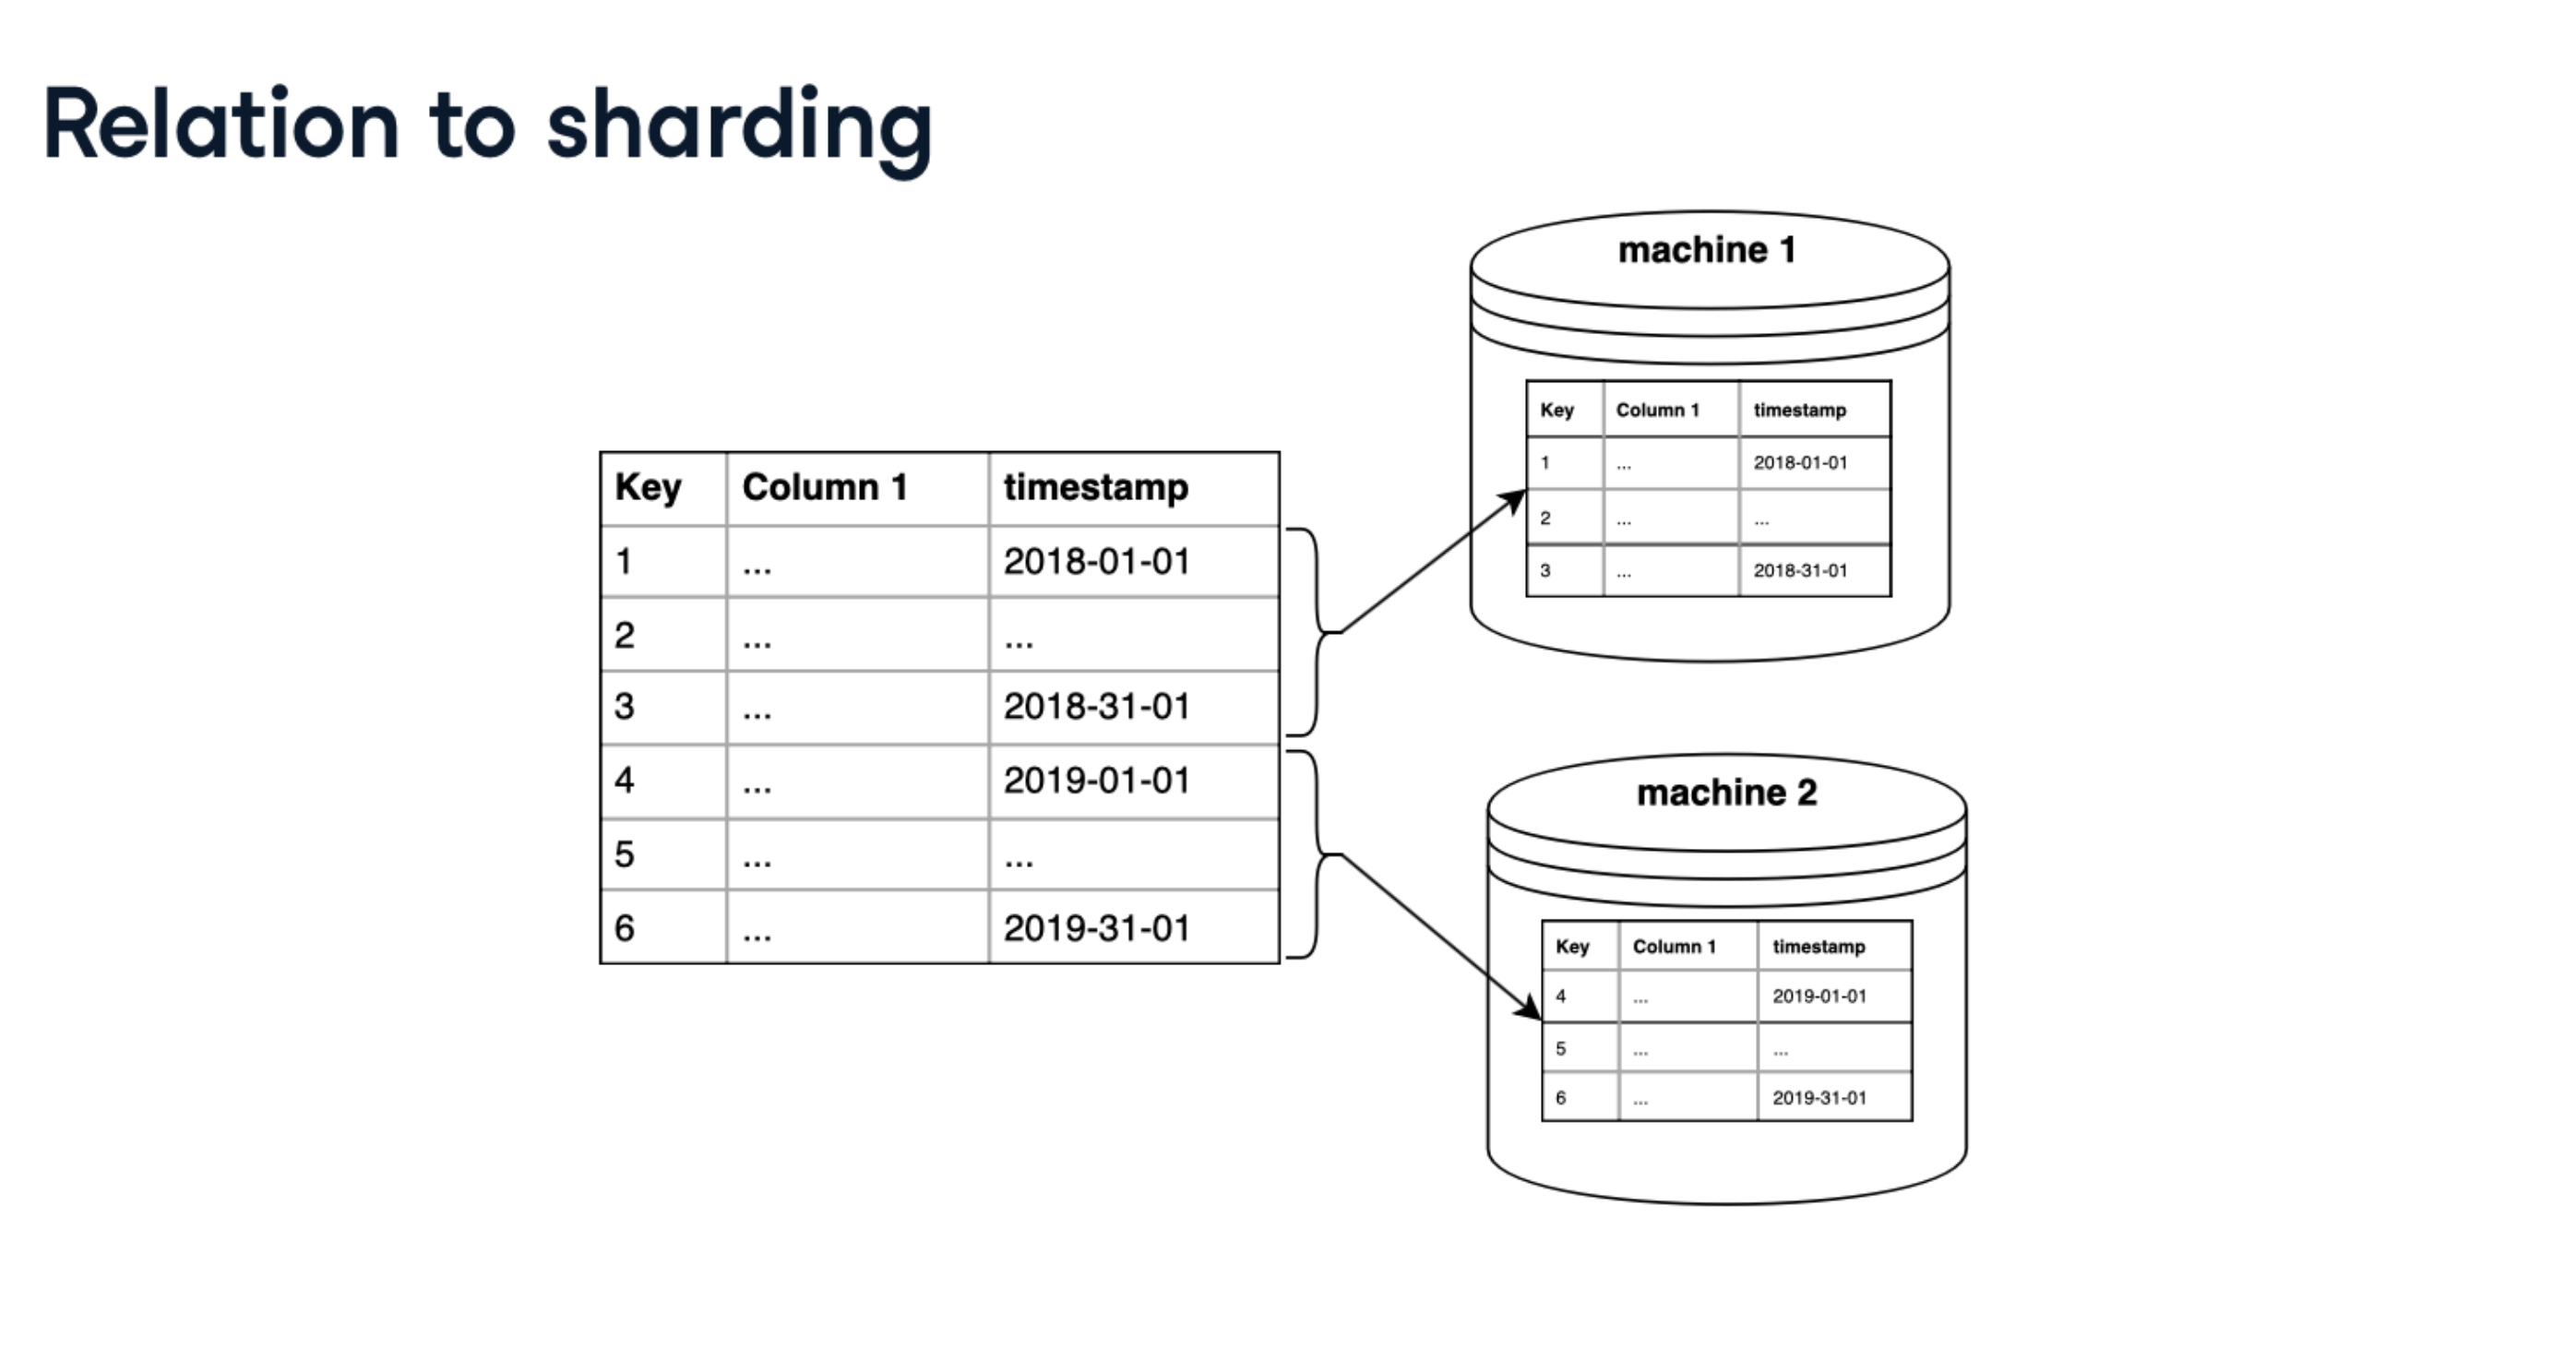
\includegraphics[width=1.0\textwidth]{figures/Sharding.png}
\end{figure}

\section{Data integration}
\subsection{Database roles and access control}